%!TEX TS-program = xelatex
%!TEX encoding = UTF-8 Unicode
\documentclass[a4paper, 12pt, oneside]{book}

\usepackage{cite}
%\usepackage{chapterbib}
%The chapterbib package facilitates multiple bibliographies in a LATEX document
\usepackage[hyphens]{url}
%Verbatim with URL-sensitive line breaks.
\usepackage[colorlinks=true,linkcolor=black,citecolor=black,filecolor=blue,urlcolor=blue,unicode]{hyperref}
%The hyperref package is used to handle cross-referencing commands in LaTeX to produce hypertext links in the document. The package provides backends for the \special set defined for HyperTeX DVI processors; for embedded pdfmark commands for processing by Acrobat Distiller (dvips and Y&Y��s dvipsone); for Y&Y��s dviwindo; for PDF control within pdfTeX and dvipdfm; for TeX4ht; and for VTeX��s pdf and HTML backends.

\usepackage{verbatim}
%The verbatim environment  simply reproduces every character you input, including all  s p a c e s!
\usepackage{color}
%you can set the color of the font of the text, and set the background color of the page.
\usepackage[dvipsnames]{xcolor}
%xecolor package is a simple package which defines about 140 different colors by XeTeX's font
\usepackage{graphicx}
%Standard LaTeX graphics.
%\usepackage{array}
%The array environment is used to make a table of information, with column alignment (left, center, or right) and optional vertical lines separating the columns.
%\usepackage{gensymb}
%Provides generic commands \degree, \celsius, \perthousand, \micro and \ohm which work both in text and maths mode.
\usepackage{indentfirst}
%Make the first line of all sections etc., be indented by the usual paragraph indentation. This should work with all the standard document classes. This minimalist package is part of the "tools" bundle in the LaTeX required distribution.
%\usepackage{algorithm}
%\usepackage{algpseudocode}
%A suite of tools for typesetting algorithms in pseudo-code. The algorithmicx package provides many possibilities to customize the layout of algorithms. You can use one of the predefined layouts (pseudocode, pascal and c and others), with or without modifications, or you can define a completely new layout for your specific needs.
\usepackage{enumitem}
%Control layout of itemize, enumerate, description.  It supersedes both enumerate and mdwlist (providing well- structured replacements for all their funtionality), and in addition provides functions to compute the layout of labels, and to 'clone' the standard environments, to create new environments with counters of their own.
\usepackage{mfirstuc}
%\makefirstuc{�qstuff �r} This makes the first object of �qstuff �r uppercase unless �qstuff �r starts with a con- trol sequence followed by a non-empty group, in which case the first object in the group is converted to uppercase.
\usepackage{fancyvrb}
%This package provides very sophisticated facilities for reading and writing ver- batim TEX code.
\usepackage{amsfonts}
%TeX fonts from the American Mathematical Society.
\usepackage{ifmtarg}
%If-then-else command for processing potentially empty arguments.
\usepackage{amsmath}
%The amsmath package is a LATEX package that provides miscellaneous enhance- ments for improving the information structure and printed output of documents that contain mathematical formulas.
\usepackage{amssymb}
% Math symbols
\usepackage[mathcal]{euscript}
%This file sets up some font shape definitions to use the Euler script symbols in math mode.
\usepackage[notbib]{tocbibind}
%Add (or disable) bibliography/index/contents to Table of Contents.
\usepackage{rotating}
%Rotation tools, including rotated full-page floats.
%\usepackage{hhline}
%The command \hhline produces a line like \hline, or a double line like \hline\hline, except for its interaction with vertical lines. The command takes a preamble (rather like the preamble of a tabular environment), and this specifies whether there are to be one or two horizontal lines, and what happens when the horizontal line meets a vertical one. The package is part of the tools bundle in the LaTeX required distribution.
\usepackage{wallpaper}
%Easy addition of wallpapers (background images) to LaTeX documents, including tiling.
\usepackage{pdfpages}
%Include PDF documents in LaTeX.
\usepackage{pst-fractal,pst-exa}
% The package will draw the Julia and Mandelbrot sets, the Sierpinski triangle, Koch flake, and Apollonius Circle as well as fractal trees (which need not be balanced) with a variety of different parameters (including varying numbers of iterations).

%Define \XeTeX \XeLaTeX command
\def\reflect#1{{\setbox0=\hbox{#1}\rlap{\kern0.5\wd0
 \special{x:gsave}\special{x:scale -1 1}}\box0 \special{x:grestore}}}
\def\XeLaTeX{\leavevmode
 \setbox0=\hbox{X\lower.5ex\hbox{\kern-.15em\reflect{E}}\kern-.08em\LaTeX}%
 \dp0=0pt\ht0=0pt\box0}
 \def\XeTeX{\leavevmode
 \setbox0=\hbox{X\lower.5ex\hbox{\kern-.15em\reflect{E}}\kern-.08em\TeX}%
 \dp0=0pt\ht0=0pt\box0}

% \usepackage[none]{hyphenat}  %hyphenation package

% Start Declare physics symbols
\newcommand{\gv}[1]{\ensuremath{\mbox{\boldmath$ #1 $}}} 
\newcommand{\grad}[1]{\gv{\nabla} #1} % for gradient
\let\divsymb=\div % rename builtin command \div to \divsymb
\renewcommand{\div}[1]{\gv{\nabla} \cdot #1} % for divergence
\newcommand{\curl}[1]{\gv{\nabla} \times #1} % for curl
\let\baraccent=\= % rename builtin command \= to \baraccent
\renewcommand{\=}[1]{\stackrel{#1}{=}} % for putting numbers above =
%end Declare

\usepackage{booktabs}				% ����u��
\usepackage{tabularx}
%tabularx, is defined, which takes the same arguments as tabular*, but modifies the widths of certain columns, rather than the inter column space, to set a table with the requested total width. The columns that may stretch are marked with the new token X in the preamble argument. This package requires the array package. The package is part of the tools bundle in the LaTeX required distribution.
%\usepackage{lmodern}
%The Latin Modern family of fonts consists of 72 text fonts and 20 mathematics fonts, and is based on the Computer Modern fonts released into public domain by AMS (copyright c 1997 AMS).
%\font\lmr="[lmroman10-regular]"

%\usepackage{listings}
%Typeset source code listings using LaTeX.
%\usepackage{textcomp}
%provide many text symbols (such as baht, bullet, copyright, musicalnote, onequarter, section, and yen)

\usepackage{amsthm}
%The package facilitates the kind of theorem setup typically needed in American Mathematical Society publications. The package offers the theorem setup of the AMS document classes (amsart, amsbook, etc.) encapsulated in LaTeX package form so that it can be used with other document classes. Amsthm is part of the (required) AMS-LaTeX distribution, so should be present in any LaTeX distribution.
\newtheorem{mydef-no-caption}{Definition}
\newenvironment{mydef}[1][]%
	{\begin{mydef-no-caption}{\ifnotmtarg{#1}{\textnormal{(\textbf{#1})}~}}}%
	{\end{mydef-no-caption}}

\usepackage{numprint}
%Print numbers with separators and exponent if necessary.
\npthousandsep{,}
\npthousandthpartsep{}
\npdecimalsign{.}

\usepackage{multirow}
%Create tabular cells spanning multiple rows.

\usepackage{ntu}
%NTU thesis style file
\hypersetup{
	pdfauthor={\authorEN{}},
	pdftitle={\titleEN{}},
	pdfsubject={NTU Thesis}
}

\usepackage{setspace}
%Set space between lines.

\usepackage[absolute]{textpos}
%Place boxes at arbitrary positions on the LaTeX page.
\lstdefinestyle{nonumbers}{numbers=none}
\textblockorigin{0mm}{0mm}

\setcounter{tocdepth}{2}

\pagestyle{plain}

\usepackage{CJKnumb}
\usepackage{titletoc}					% 目錄修改套件
\usepackage{titlesec} 				% 美化章節標題套件

% === 圖表相關設定 ===

\graphicspath{{images/}} 			% 設定圖形路徑

\newcommand{\loflabel}{圖}
\newcommand{\lotlabel}{表}
\renewcommand\figurename{\loflabel}
\renewcommand\tablename{\lotlabel}
\setlength{\abovecaptionskip}{10pt} % 修改圖表標題和圖表內容的間距
\setlength{\belowcaptionskip}{10pt} % 修改圖表標題和圖表內容的間距

% === 自訂指令 ===
\renewcommand\contentsname{目錄}
\renewcommand\listfigurename{圖目錄}
\renewcommand\listtablename{表目錄}
\renewcommand\bibname{參考文獻}

\setlength{\parindent}{22pt}  	% 設定縮排

\newboolean{isAppendix}
\setboolean{isAppendix}{false}


% === 目錄標題 (配合 titletoc) ===
\titlecontents{chapter}[0em]{\fontsize{12}{18}\selectfont}
  {\hspace{3.5em}\contentslabel[第\CJKnumber{\thecontentslabel}章]{3.5em}}
  {}{\hspace{0.5em}\titlerule*{.}\contentspage}

\titlecontents{section}
[3.5em]
{\fontsize{12}{18}\selectfont}
{\contentslabel{2em}}
{}{\hspace{0.5em}\titlerule*{.} \contentspage}

\titlecontents{subsection}
[6.5em]
{\fontsize{12}{18}\selectfont}
{\contentslabel{3em}}
{}{\hspace{0.5em}\titlerule*{.} \contentspage}

% === 章節標題 (配合 titlesec) ===
\titleformat{\chapter}[display]
	{\bf\Large}
	{\filleft 第\,\CJKnumber{\thechapter}\,章}
	{1ex}
	{\huge\titlerule
	 \vspace{2ex}%
	 \filright}
	[\vspace{2ex}%
	 \titlerule]


% \usepackage{notoccite}
\usepackage{longtable}
\usepackage{caption}
\usepackage{siunitx,array,multirow}
\usepackage{arydshln,diagbox}

\begin{document}

\setcounter{tocdepth}{3}
\setcounter{secnumdepth}{3}

%----------- hyphenation  -----------
%\righthyphenmin=10  % Best hyphenation parameter

%----------- watermark -----------
\CenterWallPaper{0.174}{watermark.pdf}
\setlength{\wpXoffset}{6.1725cm}
\setlength{\wpYoffset}{10.5225cm}

%----------- cover page -----------
\maketitle

%----------- side page, used for printing on spline -----------
% \makeside


\frontmatter
%----------- generate the certification page by LaTeX -----------
%\makecertification
%----------- includepdf by using package pdfpages -----------
%\addcontentsline{toc}{chapter}{口試委員會審定書}
%\includepdf[pages={1}]{cert.pdf}

\includepdf[pages={1}]{Verification_Letter.pdf}
\onehalfspacing
\begin{acknowledgementsCH}
 這裡將簡單介紹如何利用\LaTeX\ 來編輯你的畢業論文,若不知道\LaTeX\ 是什麼或是沒有概念的話,建議你可以簡單看過放在此資料夾裡的\href{run:./latex123.pdf}{李果正-大家來學\LaTeX}前四章內容,在下載適合的\LaTeX\ 整合發行套件之後(請看第~\ref{it:download}項),可以嘗試用剛安裝好的\LaTeX\ 編輯器來編譯\href{run:./thesis.tex}{thesis.tex}這份文件,編譯的方法可以看下面第~\ref{it:comp}項的介紹,若編譯成功,所編譯出來的thesis.pdf文件的應該會跟此demo.pdf文件一模一樣,而且沒有任何問號符號,走到這一步的話,就差不多可以開始邊學習\LaTeX\ 邊編輯你的畢業論文了!基本上會使用到的指令都包含在論文的的各章節裡,怎麼在論文裡寫公式或是放圖之類的就自行看tex檔學吧。如果有任何問題或建議可以來信與我討論,我的信箱是\href{mailto:dran31545@gmail.com}{dran31545@gmail.com},或是到此範本\href{http://code.google.com/p/ntu-thesis-latex-template/}{Google Project}裡面的\href{http://code.google.com/p/ntu-thesis-latex-template/issues/list}{Issues}貼上你的問題與建議,我會盡我所能更新此範本,也歡迎大家自行重製、改良此範本並散布給他人,祝大家順利畢業!\\\\
 要編輯致謝請打開\href{run:./acknowledgementsCH.tex}{acknowledgementsCH.tex}\\
 \begin{enumerate}[leftmargin=0pt, topsep=0pt, itemsep=0pt, label=\Roman{*}.]
\item 此範本參考並修改自下列網站的資料:
\begin{enumerate}[topsep=0pt, itemsep=0pt, label=$\bullet$]
    \item \href{http://www.csie.ntu.edu.tw/~tzhuan/www/resources/ntu/}{如何用 LaTeX 排版臺灣大學碩士論文}\\
    \textemdash 台灣大學論文\LaTeX\ 樣版原創者\href{http://www.csie.ntu.edu.tw/~tzhuan/www/}{黃子桓}的教學網頁
    \item \href{http://www.hitripod.com/blog/2012/05/latex-thesis-template-quick-reference/}{LaTeX 常用語法及論文範本}\\
    \textemdash \href{http://www.hitripod.com/blog/}{Hitripod}所修改的範本,這裡參考了許多他所寫的格式和內容
    \item \href{http://www.cc.ntu.edu.tw/chinese/epaper/0014/20100920_1404.htm}{使用LaTeX做出精美的論文}
    \item \href{http://www.hitripod.com/blog/2011/04/xetex-chinese-font-cjk-latex/}{XeTeX:解決 LaTeX 惱人的中文字型問題}
    \item \href{http://code.google.com/p/ntuthesis/}{台灣大學碩士、博士論文的Latex模板}\\
\end{enumerate}
\item 幾個有用的參考資料及網路資源:
\begin{enumerate}[topsep=0pt, itemsep=0pt, label=$\bullet$]
    \item \href{run:./latex123.pdf}{李果正-大家來學\LaTeX}\textemdash 建議先看完前四章
    \item \href{http://en.wikibooks.org/wiki/LaTeX}{WIKIBOOKS-\LaTeX}\textemdash 好用的線上工具書
    \item \href{run:./Working_with_a_bib_file_using_Jabref.pdf}{Working with a .bib file using JabRef}
    \item \href{run:./Fi087_S.pdf}{Using BibDesk - A short tutorial}
    \item \href{http://www.dfcd.net/articles/latex/latex.html}{LaTeX for Physicists}\\
\end{enumerate}
\item 下載\LaTeX\ 整合發行套件,可參考\href{http://www.tug.org/texcollection/}{TeX Collection}:\label{it:download}
 \begin{enumerate}[topsep=0pt, itemsep=0pt, label=\arabic{*}.]
     \item \href{http://www.tug.org/mactex/}{MacTeX}: For \textcolor{Green}{\textbf{MacOSX}},下載\href{http://mirror.ctan.org/systems/mac/mactex/MacTeX.pkg}{MacTeX.pkg}
     \item \href{http://www.tug.org/protext/}{ProTeXt}: For \textcolor{Green}{\textbf{Windows}},下載\href{ftp://ftp.fernuni-hagen.de/pub/windows/win32/ProTeXt/}{ISO file}
     \item \href{http://www.tug.org/texlive/}{TeX Live}: For \textcolor{Green}{\textbf{GNU/Linux}} and \textcolor{Green}{\textbf{MacOSX}}, and \textcolor{Green}{\textbf{Windows}},下載\href{http://www.tug.org/texlive/acquire-iso.html}{ISO file}
     \item \href{http://ctan.org/}{CTAN}: The Comprehensive TeX Archive Network.\\
 \end{enumerate}

\item 好用的程式:
 \begin{enumerate}[topsep=0pt, itemsep=0pt, label=$\bullet$]
    \item 文獻管理系統:
        \begin{enumerate}[topsep=0pt, itemsep=0pt, label=\arabic{*}.]
         \item \href{http://jabref.sourceforge.net/}{JabRef}\\
                     可參考\href{run:./Working_with_a_bib_file_using_Jabref.pdf}{Working with a .bib file using JabRef}或是\href{https://www.google.com/search?q=jabref}{Google}及\href{http://www.youtube.com/results?search_query=jabref}{YouTube}
         \item \href{http://bibdesk.sourceforge.net/}{BibDesk} (For Mac)\\
                     可參考\href{run:./Fi087_S.pdf}{Using BibDesk - A short tutorial}或是\href{https://www.google.com/search?q=bibdesk}{Google}及\href{http://www.youtube.com/results?search_query=bibdesk}{YouTube}
         \end{enumerate}
         \item 方程式編輯器:\href{https://chrome.google.com/webstore/detail/dinfmiceliiomokeofbocegmacmagjhe?hl=zh-TW}{Daum Equation Editor} (Chrome App,必須使用Google瀏覽器)\\
 \end{enumerate} 
\item 編譯流程:\label{it:comp}
\begin{enumerate}[topsep=0pt, itemsep=0pt, label=\arabic{*}.]
    \item \texttt{xelatex thesis}\\ 對thesis.tex進行第一次XeLaTeX編譯,產生thesis.pdf以其他檔案
    \item \texttt{bibtex thesis}\\ 對thesis.tex進行BibTeX編譯,產生bbl檔以及blg檔
    \item \texttt{xelatex thesis}\\ 對thesis.tex進行第二次XeLaTeX編譯,產生目錄、圖表連結及參考文獻
    \item \texttt{xelatex thesis}\\ 對thesis.tex進行第三次XeLaTeX編譯,產生參考文獻連結,完成編譯
\end{enumerate} 
    \textcolor{Red}{注意!}此範本使用cite套件,可依據你利用文獻管理系統所整理好的\href{run:./thesisbib.bib}{thesisbib.bib}檔在論文最後產生參考文獻頁面,若你的系所規定要在每個章節的後面產生參考文獻,則可以用chapterbib套件,來對每個有附參考文獻的章節tex檔進行一次BibTeX編譯產生bbl檔,如範例的\href{run:./introduction.tex}{introduction.tex}、\href{run:./THM.tex}{THM.tex}和\href{run:./EXP.tex}{EXP.tex},如果有這需要請把\href{run:./thesis.tex}{thesis.tex}檔裡使用cite套件的指令利用註解符號\texttt{\%}來取消使用cite套件,並刪去出現在使用chapterbib套件指令前面的註解符號\texttt{\%}來啟動使用chapterbib套件
    \begin{verbatim}
\usepackage{cite}
%\usepackage{chapterbib}
改成
%\usepackage{cite}
\usepackage{chapterbib}
    \end{verbatim}
    再來利用註解符號\texttt{\%}取消會把參考文獻放在論文最後的指令
    \begin{verbatim}
\bibliographystyle{unsrt}
\addcontentsline{toc}{chapter}{\bibname}
\bibliography{thesisbib}
改成
%\bibliographystyle{unsrt}
%\addcontentsline{toc}{chapter}{\bibname}
%\bibliography{thesisbib}
    \end{verbatim}
    再把用來輸入章節檔案的\texttt{\textbackslash input}指令改成\texttt{\textbackslash include}指令
     \begin{verbatim}
\input{introduction}  =>  \include{introduction}
\input{THM}           =>  \include{THM}
\input{EXP}           =>  \include{EXP}
     \end{verbatim}
    最後記得在每個有附參考文獻的章節加上產生參考文獻的指令,即在\href{run:./introduction.tex}{introduction.tex}、\href{run:./THM.tex}{THM.tex}和\href{run:./EXP.tex}{EXP.tex}三個檔案裡最後啟動下面兩行指令
     \begin{verbatim}
%\bibliographystyle{unsrt} => \bibliographystyle{unsrt}
%\bibliography{thesisbib}  =>  \bibliography{thesisbib}
     \end{verbatim}
    而編譯時則需要對有附參考文獻的\href{run:./introduction.tex}{introduction.tex}、\href{run:./THM.tex}{THM.tex}和\href{run:./EXP.tex}{EXP.tex}各做一次BibTeX 編譯,編譯流程如下
    \begin{enumerate}[topsep=0pt, itemsep=0pt, label=\arabic{*}.]
    \item \texttt{xelatex thesis}\\ 對thesis.tex進行第一次XeLaTeX編譯,產生thesis.pdf及其他檔案
    \item \texttt{bibtex introduction}\\ 對introduction.tex進行BibTeX編譯,產生bbl檔以及blg檔
    \item \texttt{bibtex THM}\\ 對THM.tex進行BibTeX編譯,產生bbl檔以及blg檔
    \item \texttt{bibtex EXP}\\ 對EXP.tex進行BibTeX編譯,產生bbl檔以及blg檔
    \item \texttt{xelatex thesis}\\ 對thesis.tex進行第二次XeLaTeX編譯,產生目錄、圖表連結及參考文獻
    \item \texttt{xelatex thesis}\\ 對thesis.tex進行第三次XeLaTeX編譯,產生參考文獻連結,完成編譯\\
\end{enumerate} 
\item 補充說明與注意事項:
\begin{enumerate}[topsep=0pt, itemsep=0pt, label=$\bullet$]
    \item 口試委員會審定書:\\
    請到台大圖書館網頁的\href{http://etds.lib.ntu.edu.tw/etdsystem/submit/submitLogin}{電子論文服務}下載\href{http://gra103.aca.ntu.edu.tw/gra2007/gra/tienn/\%E5\%AD\%B8\%E4\%BD\%8D\%E8\%80\%83\%E8\%A9\%A6\%E8\%A1\%A8\%E5\%86\%8A/THESISSAMPLE.DOC}{論文格式範本},並修改成正確的格式,也可到此範本所在資料夾的\href{run:./cert.doc}{cert.doc}修改。當然你也可以利用LaTeX來編輯,你只要填好\href{run:./ntuvars.tex}{ntuvars.tex}檔的資料,並去除在thesis.tex裡下面這行的註解符號\texttt{\%} 
    \begin{verbatim}
%\makecertification
    \end{verbatim}
    編譯完後就可以產生審定書格式。口試通過後,請把已經簽名的審定書掃描成pdf檔,再取代原本的\href{run:./cert.pdf}{cert.pdf},即可放上已簽名的審定書。處理審定書出現的指令在thesis.tex裡 
    \begin{verbatim}
%----------- generate the certification ...
%\makecertification
%----------- includepdf by using package ...
\addcontentsline{toc}{chapter}{口試委員會審定書}
\includepdf[pages={1}]{cert.pdf}
    \end{verbatim}
    \item 浮水印:\\
    資料夾已經附上浮水印檔案了,若學校有更改,到請到台大圖書館網頁的\href{http://etds.lib.ntu.edu.tw/etdsystem/submit/submitLogin}{電子論文服務}下載\href{http://etds.lib.ntu.edu.tw/files/watermark.pdf}{pdf格式的浮水印}到此範本所在資料夾。若要開啟關閉浮水印功能,即自行刪去或加上下面位於\href{run:./thesis.tex}{thesis.tex}指令的註解符號\texttt{\%}
    \begin{verbatim}
%\CenterWallPaper{0.174}{watermark.pdf}
%\setlength{\wpXoffset}{6.1725cm}
%\setlength{\wpYoffset}{10.5225cm}
    \end{verbatim}
    \item 單面印刷與雙面印刷:\\
    此範本為單面印刷,若論文頁數超過80頁,依規定需要用雙面印刷,此時只需把thesis.tex裡的
    \begin{verbatim}
\documentclass[a4paper, 12pt, oneside]{book}
改成
\documentclass[a4paper, 12pt, twoside]{book}
    \end{verbatim}
        \item 如何加入附錄?\\
    在\href{run:./thesis.tex}{thesis.tex}裡,依需求選擇input或include,刪去\texttt{\%}符號來輸入附錄章節
    \begin{verbatim}
%----------- Input your appendix here  -----------
%\chapter{附錄:程式碼說明}

\hspace*{-3cm}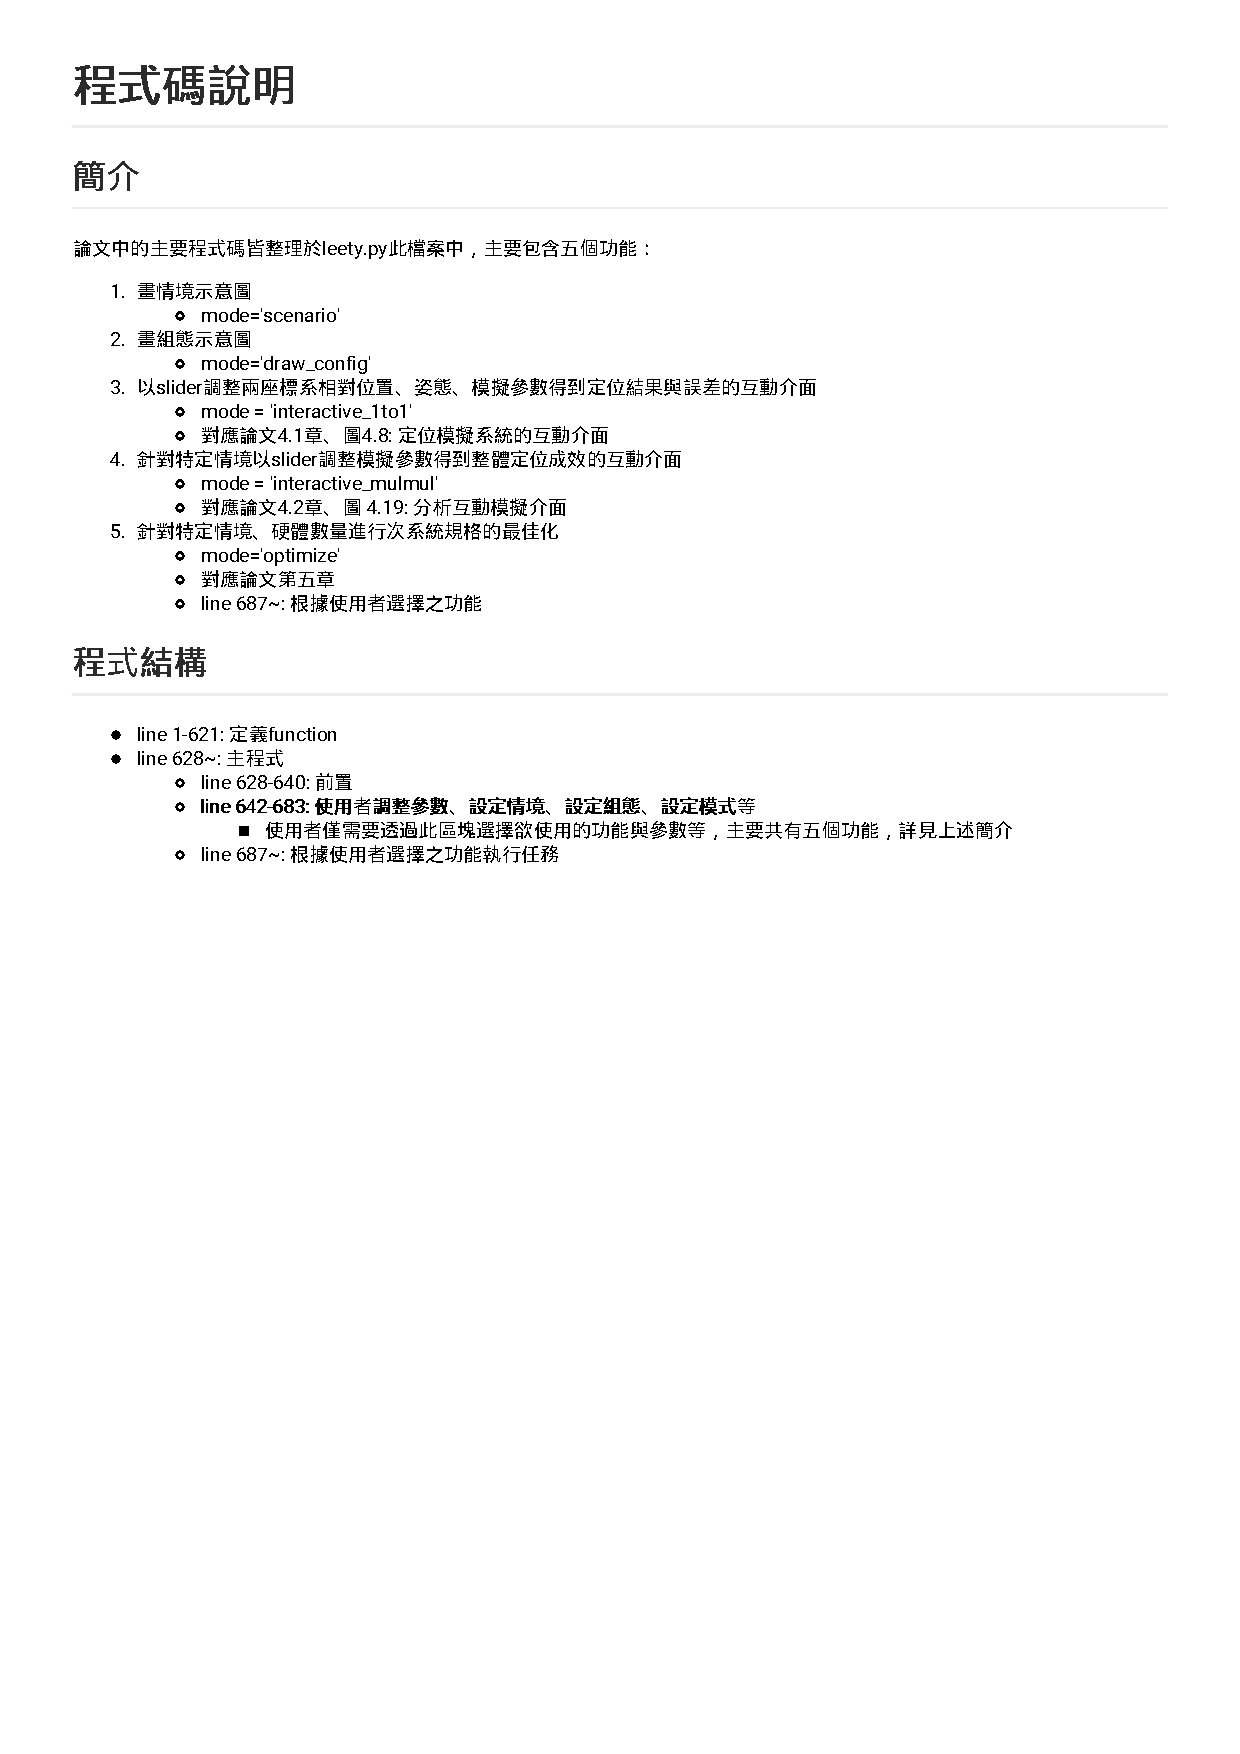
\includegraphics[width=22cm]{ReadMe.pdf}
%or %chapter cite  == \include
%\chapter{附錄:程式碼說明}

\hspace*{-3cm}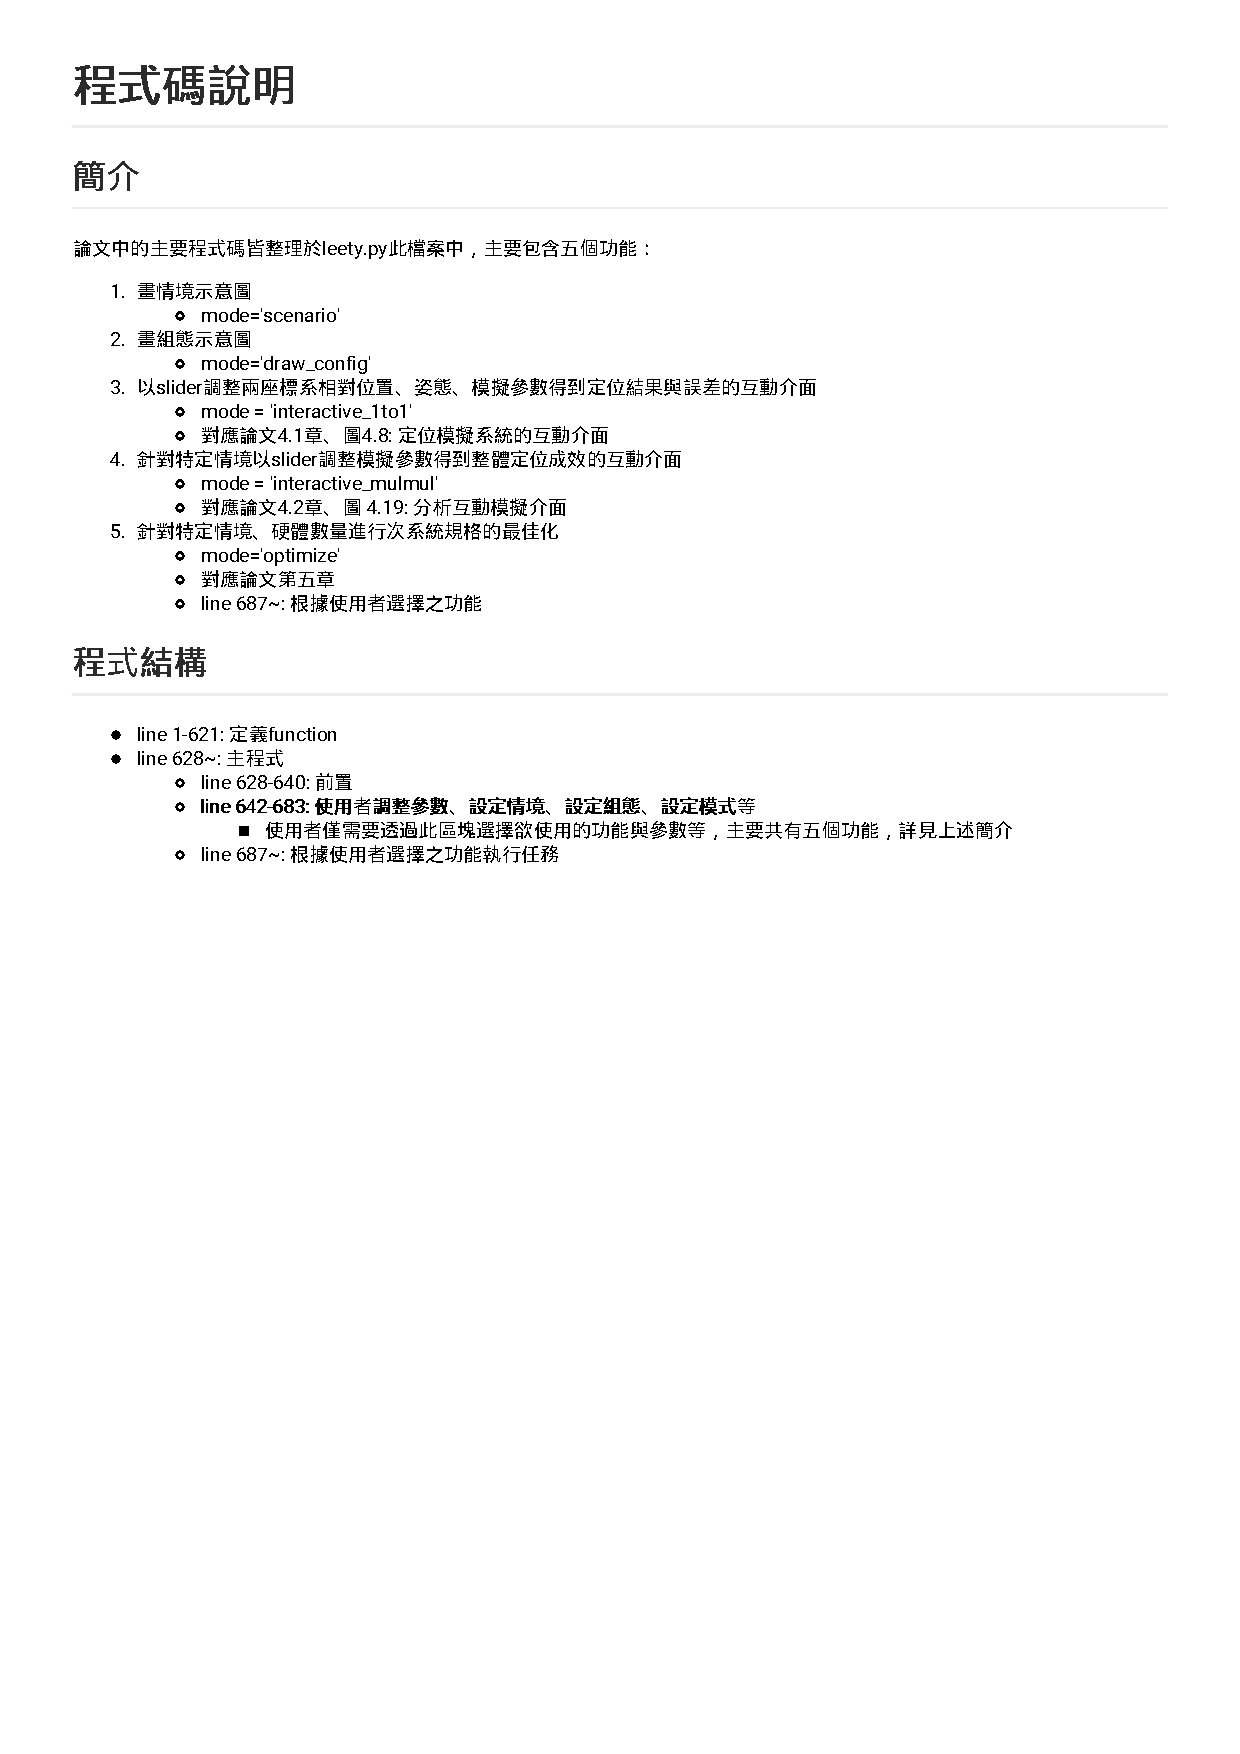
\includegraphics[width=22cm]{ReadMe.pdf}
    \end{verbatim}
    在章節檔\texttt{AppendixA.tex}裡,開頭打
    \begin{verbatim}
\chapter{First appendix title}
    \end{verbatim}
    即可,以此類推。    
        \item 系上規定論文圖表須全部放到最後獨立出來的章節,且章節不出現在目錄中:\\
    在\href{run:./thesis.tex}{thesis.tex}裡,依需求選擇input或include,刪去\texttt{\%}符號來輸入圖表章節
    \begin{verbatim}    
%----------- Input your Figure chapter here  -----------
%\input{EndFigTab} 
%chapter cite  == \include
%\include{EndFigTab}
    \end{verbatim}
    在章節檔\href{run:./EndFigTab.tex}{EndFigTab.tex}裡有範例和說明可供參考,要注意正文的圖表和附錄的圖表要分清楚,即在\href{run:./EndFigTab.tex}{EndFigTab.tex}內
    \begin{verbatim}    
\renewcommand{\thefigure}{\arabic{chapter}.\arabic{figure}} 
\renewcommand{\thetable}{\arabic{chapter}.\arabic{table}} 
%--- Input your main figures and tables here  ---
    \end{verbatim}
    這幾行之後章節計數器格式已切換為1\dots 9,放正文的圖表 ,
     \begin{verbatim}    
\renewcommand{\thefigure}{\Alph{chapter}.\arabic{figure}} 
\renewcommand{\thetable}{\Alph{chapter}.\arabic{table}}
%--- Input your appendix figures and tables here  ---
    \end{verbatim}
    這幾行之後章節計數器格式已切換為A\dots Z,放附錄的圖表。另外要取消圖表的浮動功能,才能讓圖表按照指令出現順序排好,即把平常使用的圖表指令
    \begin{verbatim}    
\begin{figure}[htb]
...
\begin{table}[htb]
    \end{verbatim}
    改成
     \begin{verbatim}    
\begin{figure}[!]
...
\begin{table}[!]
    \end{verbatim}
    剩下的只要注意章節圖表的計數器設定即可。\texttt{\textbackslash ref}和\texttt{\textbackslash label}指令可以在此圖表章節與正文章節使用。
     \item 如果我想要修改margin(文字邊界)的話,可以從哪裡下手呢?\\
     請打開\href{run:./ntu.sty}{ntu.sty}修改下面這行的上下左右參數即可:
    \begin{verbatim}
\RequirePackage[top=3cm,left=3cm,bottom=2cm,right=3cm]{geometry}
    \end{verbatim}
    \item 我想引用Twomey (1974): Pollution and planetary albedo這篇論文,如何用\texttt{\textbackslash cite}引用它的時候在內文顯示Twomey (1974) [編號] ?\\
    建議使用natbib套件,參考資料如下:\\
    \href{http://en.wikibooks.org/wiki/LaTeX/Bibliography_Management}{LaTeX/Bibliography Management}\\
    \href{http://nodonn.tipido.net/bibstyle.php}{Overview of Bibtex-Styles}\\
    \href{http://merkel.zoneo.net/Latex/natbib.php}{Reference sheet for natbib usage }\
 \item \XeTeX\ :\\
    此範本中文字體使用\XeTeX\ 轉換,細節請參考\href{http://www.hitripod.com/blog/}{Hitripod}寫的\href{http://www.hitripod.com/blog/2011/04/xetex-chinese-font-cjk-latex/}{ 
XeTeX:解決 LaTeX 惱人的中文字型問題}。
 \item 如何輸入英文`單引號'和``雙引號''以及不同長度的破折號?\\
        可以參考\href{run:./latex123.pdf}{李果正-大家來學\LaTeX}第17頁針對標點符號的遊戲規則,範例如下,輸入以下指令:\\
        \begin{verbatim}
`單引號'\\
``雙引號''\\
-hyphen\\
--en-dash\\
---em-dash\\
        \end{verbatim} 
        則顯示:\\
       `單引號'\\
        ``雙引號''\\
        -hyphen\\
        --en-dash\\
        ---em-dash\\
    \end{enumerate} 
    \end{enumerate} 
               

%----------- Have a fractal fern? -----------
%\begin{pspicture}
%\psFern[scale=30,maxIter=100000,linecolor=Green]
%\end{pspicture}

 \end{acknowledgementsCH} %致謝
\begin{abstractCH}

  隨著科技與物連網的發展,各領域對於量測資訊的需求大量增加,其中相對位置的資訊實為重要。然而,現今室內定位仍仰賴多個參考點進行定位,缺乏僅以「可攜式單位」達到兩物體之間三維定位的方法。因此,我們由探討不同的室內定位方法開始,根據以上需求將研究重點聚焦在光波段中發光二極體(Light Emitting Diode,簡稱LED)與光電二極體(Photodiode,簡稱PD)的定位方法,此方法有達到兩單位之間三維定位的潛力,但現今文獻中對使用情境與系統設計的限制仍許多,大多需限制接收與發射平面平行且僅能達到二維定位,除此之外也會對硬體進行限制。因此,本研究針對LED與PD的定位方法,建立一個可以不限制接收與發射平面平行的三維定位演算法,也不限制硬體的朗博次方(Lambertian Order)、硬體數量以及各硬體的擺放指向,使系統具有根據不同情境進行改變與設計的能力,改善此領域中對系統設計以及使用情境較多的限制。建立演算法後,本研究由該演算法建立一模擬環境與系統成效的量化方式,於模擬環境中,我們可以評估各系統設計下的定位效能,並透過改變不同的系統設計、使用情境與應用範圍(Region of Interest)、以及誤差參數,來觀察以及探討各參數對系統成效的影響。除此之外,本研究針對不同的使用情境,將系統設計作為變數進行最佳化,可將該最佳系統設計作為實際硬體系統搭建的參考。總結來說,本研究提供一僅利用兩單位進行三維定位的定位演算法,並建立一模擬環境,讓使用者得以在不浪費硬體搭建的成本下對系統設計進行分析與評估,也可以針對特定的使用情境進行系統設計的最佳化,在硬體系統搭建前達到有效的評估。

  % 此定位演算法對

  \vspace{1cm}
  \noindent \textbf{關鍵字:室內定位、光定位、發光二極體、光電二極體、定位演算法、最佳化}

\end{abstractCH}

\doublespacing
\begin{abstractEN}

    With the development of IoT, the demand of sensors and data,especially positioning information, has increased drastically. Nowadays, indoor positioning systems mostly use multiple reference points in order to obtain position information. There is no efficient way to get 3-dimensional relative position with only two portable unit. Therefore, we start from introducing different positioning methods and techniques. According to the aforementioned demand, we focused on the positioning technique of using LEDs and photodiodes. Although this technique has the potential fulfill the needs, the majority of nowadays research have restricted usage scenario and system design. Particulary, they could only obtain 2-dimensional position while restricting transmitting and receiving planes to be parralel. As a result, we developed a positioning algorithm which can abtain 3-dimensional position without planes parralel assumption. Other than this, Lambertian order, hardware amound and hardware placing direction are not constrained either, which means the system has the ability to adjust with respect to different scenario. With this positioing algorithm, we further set up a simulation environment and a method to quantify system performance. In the simulation environment, we can evaluate system performance with different system design in different scenario. By evaluation method, the influence of each system design variable and noise simulation variable can be discussed. Aside from evaluation, we also proposed a optimization method to take system design as variable and in specific scenario. Overall, we proposed a 3-dimensional positioning algorithm without parallel planes assumption while considering Lambertian order, hardware amount and placing orientation as variable. Except for positioning algorithm, the simulation environment and optimization method provide users a very a guide to construct the hardware system. 

    \vspace{1cm}
    \noindent \textbf{Key Words:Indoor Positioning, Light Positioning, Light-Emitting-Diode, Photodiode, Positioning Algorithm, Lambertian Order}

\end{abstractEN}


\doublespacing
\onehalfspacing
\tableofcontents
\listoffigures
\listoftables
\chapter*{符號列表}
\label{chp:symbol}
% \addcontentsline{toc}{chapter}{符號列表}


%英文字母 -> 希臘字母%
%小寫 -> 大寫%
%向量 -> 純量% %粗->細%


% \section*{符號列表}
\subsection*{座標系}

\begin{longtable}[l]{cl}
    % $\text{Bell}(\cdot)$ & 鐘形函式\\
    $\boldsymbol{P}$ & 座標點\\
    $x,y,z$ & 座標點$\boldsymbol{P}$的$x,y,z$分量\\
    $\boldsymbol{V}$ & 單位向量\\
    $u,v,w$ & 單位向量$\boldsymbol{V}$的$x,y,z$分量\\
    $d,\alpha,\beta$ & 單位向量$\boldsymbol{V}$在球座標系中的天頂角(Zenith Angle)、方位角(Azimuth Angle)、距離分量\\
\end{longtable}

% \begin{figure}[ht]
% 	\centering
% 	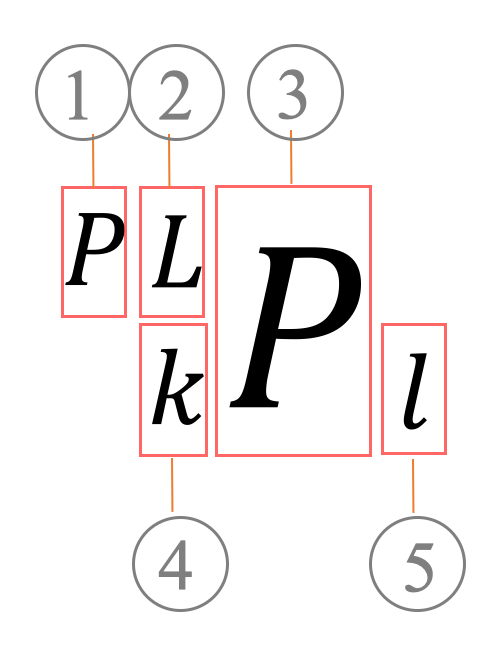
\includegraphics[width=3cm]{ch1pic/not_pos.png}
%     \caption{座標系小標解釋}
%     \label{pic:not_pos}
% \end{figure}

% \begin{description}
%     \item[(1)] 投影至的座標系($P$: PD座標系;$L$: LED座標系)
%     \item[(2)] 定義於哪個座標系($P$: PD座標系;$L$: LED座標系)
%     \item[(3)] 座標系符號(如上表)
%     \item[(4)] 第$k$個樣本點($k=1,2,...,K$)
%     \item[(5)] 第$l$個LED或第$p$個PD($l=1,2,...,L$;$p=1,2,...,P$)
% \end{description}



\onehalfspacing

\subsection*{座標系轉換}

\begin{longtable}[l]{cl}
    $\boldsymbol{H}=\left[\begin{array}{cc}
         \boldsymbol{Ro}  & \boldsymbol{T} \\
        0_{1\times3} & 1
        \end{array}\right]$ & 齊次轉換矩陣 Homogeneous Transformation Matrix\\
    $\boldsymbol{T}=\left[\begin{array}{ccc}t_x&t_y&t_z\end{array}\right]^T$ & 平移向量 Transfer Vector\\
    $\boldsymbol{T}^{sph}=\left[\begin{array}{ccc}t_d&t_{\alpha}&t_{\beta}\end{array}\right]^T$ & 平移向量以球座標系表示\\
    $\boldsymbol{Ro}=\left\{\gamma_{ij}\right\}$ & 旋轉矩陣 Rotation Matrix\\
\end{longtable}

% \begin{figure}[ht]
% 	\centering
% 	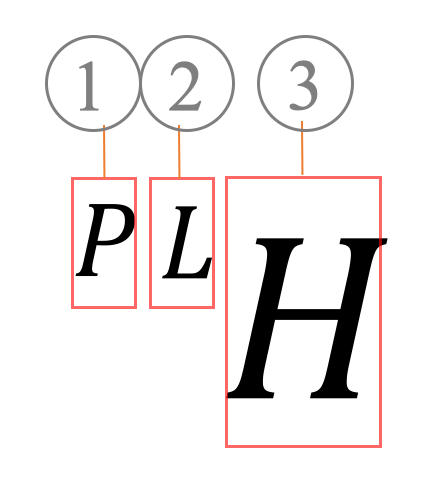
\includegraphics[width=3cm]{ch1pic/not_transform.png}
%     \caption{座標系轉換小標解釋}
%     \label{pic:not_transform}
% \end{figure}

% \begin{description}
%     \item[(1)] 投影至的座標系($P$: PD座標系;$L$: LED座標系)
%     \item[(2)] 定義於哪個座標系($P$: PD座標系;$L$: LED座標系)
%     \item[(3)] 座標系轉換符號(如上表)
%     \item[(4)] 第$k$個樣本點($k=1,2,...,K$)] 
% \end{description}




% \begin{figure}[ht]
% 	\centering
% 	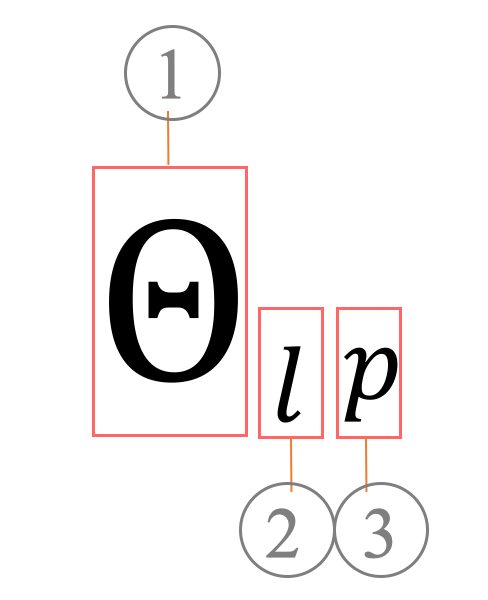
\includegraphics[width=3cm]{ch1pic/not_interactive.png}
%     \caption{LED與PD的交互關係小標解釋}
%     \label{pic:not_interactive}
% \end{figure}

% \begin{description}
%     \item[(1)] LED與PD的交互關係符號(如上表)
%     \item[(2)] 第$l$個LED($l=1,2,...,L$)
%     \item[(3)] 第$p$個PD($p=1,2,...,P$)
%     \item[(4)] 第$k$個樣本點($k=1,2,...,K$) 
% \end{description}

\onehalfspacing

\subsection*{硬體參數}

\begin{longtable}[l]{cl}
    % $\text{Bell}(\cdot)$ & 鐘形函式\\
    符號 & LED硬體參數\\ \hline
    $M\ell$ & LED的朗伯次方(Lambertian Order)\\
    $Pt$ & 總輻射通量(Total Radiation Flux) 
\end{longtable}

\begin{longtable}[l]{cl}
    % $\text{Bell}(\cdot)$ & 鐘形函式\\
    符號 & PD硬體參數\\ \hline
    $Mp$ & PD的朗伯次方(Lambertian Order)\\
    $A$ & 有效面積\\
    $Re$ & 響應率(Responsivity)\\
    $s$ &飽和電流
\end{longtable}


\onehalfspacing

\subsection*{LED與PD的交互關係}

\begin{longtable}[l]{cl}
    % $\text{Bell}(\cdot)$ & 鐘形函式\\
    $\phi$ & PD入射角\\
    $\theta$ & LED出射角\\
    $D$&距離\\
\end{longtable}

\onehalfspacing

\subsection*{光學領域單位}

\begin{longtable}[l]{cllll}
    % $\text{Bell}(\cdot)$ & 鐘形函式\\
    符號& 中文& 英文 & 單位符號&國際單位制\\\hline
    $\Omega$ & 立體角&Solid Angle& $sr$&球面度(Steradian) \\
    $\omega$ & 角度&Angle& $rad$&弧度(radian)\\
    $r$ & 半徑&Radius&  $m$ &公尺\\
    $\Phi$ & 輻射通量&Radiation Flux& $W$&瓦特(Watt)\\
    $I$ & 輻射強度&Radiation Intensity & $W\cdot sr^{-1}$&瓦特每球面度 \\
    $E$ & 輻照度&Irradiance&$W\cdot m^{-2}$ &瓦特每平方公尺\\
\end{longtable}


\onehalfspacing

\subsection*{系統與演算法}

\begin{longtable}[l]{cl}
    % $\text{Bell}(\cdot)$ & 鐘形函式\\
    $t_d$ & 兩座標系之間距離\\
    $\boldsymbol{Tv}$ & 兩座標系中對方所在方位\\
    $L,P$ & LED與PD總數\\
    $\ell,p$ & LED與PD編號\\
    $F\ell,Fp$ & 過濾後的LED與PD數量\\
    $Ra$& 餘弦比值\\
    $r_c$& 取作餘弦比值參考值的硬體編號\\
    $r_s$& 參考平面由$r_c$與$r_s$編號的硬體資訊獲得\\
    $N$& 平面法向量\\
    $Kb$&波茲曼常數(Boltzmann constant)\\
    $Te$& 溫度\\
    $B$& 頻寬(Bandwidth)\\
    $q$&電子電荷\\
    $Rs$&分路電阻(Shunt Resistance)\\
    $k,K$&樣本點編號以及樣本點總數\\

\end{longtable}




\onehalfspacing

\section*{小標解釋}

論文中由於座標系、硬體數量、樣本數量眾多,為了區分不同上下小標的意義,以圖\ref{pic:symbol}呈現各小標意思,左上標表示座標系,左下標顯示是哪個樣本,而右下標則依照物理量代表著LED或PD的編號,在LED與PD交互關係的物理量中右下標同時包含兩者的編號。

\begin{figure}[ht]
	\centering
	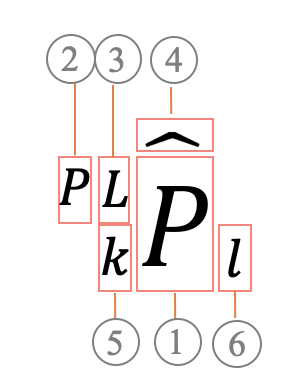
\includegraphics[width=2cm]{ch1pic/not_whole.png}
    \caption{符號小標解釋}
    \label{pic:symbol}
\end{figure}



\begin{description}
    \item[(1) 符號] 
    \item[(2) 投影至的座標系:] ($P$: PD座標系;$L$: LED座標系)
    \item[(3) 定義於哪個座標系:] ($P$: PD座標系;$L$: LED座標系)
    \item[(4) 量測訊號:] $\hat{(\cdot)}$代表該物理量為量測所得或處理量測所得訊號而得
    \item[(5) 樣本點:] 第$k$個樣本點($k=1,2,...,K$)
    \item[(6) 硬體編號:] 第$p$個PD($p=1,2,...,P$)或第$l$個LED($l=1,2,...,L$);LED與PD交互關係物理量的(6)小標為$lp$兩者的交互關係
    \item[(7) 使用的座標系統:]  以何種座標系呈現(無:卡氏座標系;$sph$:球座標系)
\end{description}


以下舉例解釋:
\begin{description}
\item[- $^{PL}_{k}\hat{\boldsymbol{T}}$:]第k個樣本點中,模擬量測方式所得到的PD座標系指向LED座標系的平移向量。

\item[- $^{L}P_l,^{PL}P_l$:]$^{L}P_l,$為第l個LED於LED座標系上的位置座標,$^{PL}P_l$則是將其投影到PD座標系上

\item[- $_{k}D_{l p}$:]第k個樣本點鐘,第l個LED與第p個PD的距離
$M\ell_l$:第l個LED的朗博次方
\end{description}
\chapter*{符號列表:依字母}
\label{chp:symbol_alphabet}
% \addcontentsline{toc}{chapter}{符號列表}


%英文字母 -> 希臘字母%
%小寫 -> 大寫%
%向量 -> 純量% %粗->細%


% \section*{符號列表}
% \subsection*{次系統座標系}
\begin{longtable}[l]{ll}
    $A$ & 有效面積\\
    $B$& 頻寬(Bandwidth)\\

    $D$&距離\\

    $E$ & 輻照度 Irradiance\\
    $Ef$&有效閥值\\
    $e$&誤差\\
    $F\ell,Fp$ & 過濾後的LED與PD數量\\
    $Gm$&多重路徑傳輸增益\\

    $I$ & 輻射強度 Radiation Intensity\\
    $Ib$&背景電流\\
    $In$&硬體誤差電流\\
    $Is$&散粒雜訊(Shot Noise)\\
    $It$&熱雜訊(Thermal Noise)\\

    $K$&樣本點總數\\
    $k$&樣本點編號\\
    $Kb$&波茲曼常數(Boltzmann constant)\\

    $\boldsymbol{H}=\left[\begin{array}{cc}
        \boldsymbol{Ro}  & \boldsymbol{T} \\
        0_{1\times3} & 1
        \end{array}\right]$ & 齊次轉換矩陣 Homogeneous Transformation Matrix\\
        
    $L$ & LED總數\\
    $\ell$ & LED編號\\

    $M\ell$ & LED的朗伯次方(Lambertian Order)\\
    $Mp$ & PD的朗伯次方(Lambertian Order)\\

    $\boldsymbol{N}$& 平面法向量\\
    $Nt$&容許範圍內樣本點數量\\

    $P$ & PD總數\\
    $p$ & PD編號\\
    $\boldsymbol{P} =
        \left[\begin{array}{ccc}
        x &y&z
       \end{array}\right]^T $ & 座標點$\boldsymbol{P}$與卡氏座標系中的$x,y,z$分量\\
    $Pt$ & 總輻射通量(Total Radiation Flux)\\ 

    $q$&電子電荷\\

    $R$&電阻\\
    $Ra$& 餘弦比值\\
    $r_c$& 取作餘弦比值參考值的硬體編號\\
    $Re$ & 響應率(Responsivity)\\
    $\boldsymbol{Ro}=\boldsymbol{Rz}(rz)\boldsymbol{Ry}(ry)\boldsymbol{Rx}(rx)$ & 
        旋轉矩陣$\boldsymbol{Ro}$以翻滾角$rx$(Roll)、俯仰角$ry$(Pitch)\\
        & 、偏航角定義$rz$(Yaw)\\%\left\{\gamma_{ij}\right\} 
    $r_s$& 參考平面由$r_c$與$r_s$編號的硬體資訊獲得\\

    $r$ & 半徑\\

    $S$ &飽和電流\\

    $\boldsymbol{T}=\left[\begin{array}{ccc}t_x&t_y&t_z\end{array}\right]^T$ & 平移向量 Transfer Vector\\
    $\boldsymbol{T}^{sph}=\left[\begin{array}{ccc}t_d&t_{\alpha}&t_{\beta}\end{array}\right]^T$ & 平移向量以球座標系中的距離$t_d$、天頂角$t_{\alpha}$、方位角$t_{\beta}$分量\\
    $Te$& 溫度\\
    $Th$& 閥值\\
    $To$&容許範圍\\
    $\boldsymbol{Tv}^{sph}=\left[\begin{array}{ccc}1&t_{\alpha}&t_{\beta}\end{array}\right]^T$ & 方位(單位平移向量)與球座標系中分量\\


    $\boldsymbol{V} =
        \left[\begin{array}{ccc}
        u &v&w
        \end{array}\right]^T$ & 指向向量$\boldsymbol{V}$與卡氏座標系中的$x,y,z$分量\\
    $\boldsymbol{V}^{sph} =
        \left[\begin{array}{ccc}
        d &\alpha&\beta
        \end{array}\right]^T$ & 指向向量$\boldsymbol{V}$與球座標系中的距離、天頂角(Zenith Angle)、\\
        &方位角(Azimuth Angle)分量\\
   
    $\theta$ & LED出射角\\
    $\Phi$ & 輻射通量 Radiation Flux\\
    $\phi$ & PD入射角\\
    $\Omega$ & 立體角 Solid Angle\\
    $\omega$ & 角度\\
\end{longtable}




\mainmatter

%\doublespacing

%----------- Include/Input your thesis here -----------
%normal cite == \input
\chapter{緒論}

% 標題: (近紅外光)任兩點 LED與光電二極體 室內 任兩點 三維相對位置 最佳化組態

\section{前言} %(工業4.0的篇幅)

隨著工業4.0的發展,機器、人與環境之間的交互互動愈發頻繁,萬物互連的背景之下,各領域對於量測資訊的需求大量增加,其中了解位置資訊為機器與人類進行判斷與計算的基礎。若能掌握空間中某特定物與自己的相對位置資訊,則可幫助新型載具、機械手臂與人類進行決策與執行任務,例如載具了解其他載具的位置、飛行器與遙控計之間的定位、智能載具與照護目標物的互動、機械手臂與夾取目標物的定位等。綜上所述,獲取兩物之間的相對位置資訊,有其必要性。

% 補iot的圖




\subsection{室內定位簡介}
% 室內定位的簡介:(範圍對點、點對點、應用情境)
現今室外定位主要仰賴全球衛星定位系統(GPS),然而礙於衛星訊號受建築物體遮蔽的特性,GPS定位技術無法應用在室內場域,因此發展一有效的室內定位方法獲得許多討論與研究關注。室內定位主要面對的困難與室外不同,較多的障礙物、牆壁、人員物體的密集度使多重路徑傳輸(Multipath propagation)影響大,也使訊號衰減與散射嚴重,以上議題都會增加誤差,且室內應用所需求的精度大多高於GPS,因此如
何設計合適的室內定位系統近年來受到研究矚目\cite{survey_indoor2014}。

室內定位最常見的分類方式為技術(Technology)與方法(Technique)\cite{survey_indoor2018},技術針對所使用的訊號與硬體種類進行分類,例如相機、紅外線、WiFi、藍芽等不同技術;而方法則是探討不同訊號皆收與處理的方式,如RSS(Received Signal Strength)與ToF(Time-of-Flight)兩種訊號接收方式,以及三邊量測法(Trilateration)、三角測量法(Triangulation)等取得相對位置訊號的方法。

\newpage

在選擇合適的技術與方法以設計室內定位系統時,需考量許多面向:

\begin{description}
    \item[量測範圍與精度] 
    包含精度、覆蓋範圍(Coverage)、目標偵測距離
    \item[成本] 
    包含硬體設備成本、系統能耗等
    \item[靈活度] 
    硬體大小、拆裝方便性、所需校正時間
    \item[是否定位可視範圍外] 
    若要進行非可視範圍(NLoS)內的定位,需利用可穿透障礙物的訊號,並犧牲精度。
    \item[是否進行即時應用] 
    若要進行即時應用,量測數據處理速度需夠快以避免訊號延遲,需犧牲訊號處理的複雜度及其附加的精度提升可能性。
    \item[目標物是否為特定物] 
    若目標物為特定某物體,則系統需有分辨訊號發送者的能力,例如無線電波的加密技術,反之光達僅有分辨訊號的有無,難以進行目標物辨識。
    \item[目標物式否有欲先安裝之特徵點] 
    是否能對目標物預先安裝特徵點也會影響系統設計,無法預先安裝特徵點的例子為自駕車,其需在陌生環境中以相機辨識周遭物體為人車或是建築物並進行定位;反例則為安裝在欲追蹤物體上的Airtag,其發送訊號以利手機追蹤並定位。 
    \item[對環境的理解程度]    
    大多WiFi與藍芽技術使用指紋比對(Fingerprinting)的方法,將系統設置完成後,預先進行大量的訊號蒐集,將接收訊號與數據庫比對得出位置,然而此方法並不能適應環境的改變,但凡環境與系統異動則原數據庫失效。  
\end{description}


礙於如此多的特性與面向,一個面面俱到的方案是不存在的。因此在設計系統時,了解不同做法的優缺點,並了解系統目標情境與需求,進而對不同設計參數做出取捨,是完成有效室內定位系統的關鍵之一\cite{survey_indoor2018}。





\section{研究動機:情境描述}
% 前言
室內定位的方法分成許多種,根據不同的應用需求與特性適用的方式也不盡相同。本研究主要目標為研究一移動物對另一特定物的相對定位方法,希望能將感測器與訊號發射器包裝成安裝方便的單位,提供一量測單位與一被量測單位,能夠靈活的將兩單位各自安裝在量測物與目標物上,在不同場域下進行三維的相對定位量測。

為更具體呈現目標的使用情境,以下舉實例描述:
\begin{description}
    \item[智慧工廠] (待補)
    \item[智慧病房] (待補)
    \item[其他]  
    智能載具與服務目標的定位、輔助視障者理解移動方向、機場內針對什麼的量測 
\end{description}

% 補實例圖




%[看最後能不能凹到一開始發想是在醫療器具上,結合實驗室研究,這樣可見光就變更合理了]

\section{研究目的}

雖然室內定位這個領域已經有許多文獻探討,然而針對此情境仍沒有一個合適的方案,因此研究目的歸納如下:

% 目標:低成本、不受環境影響、可分辨目標物、快速

\begin{itemize} 
    \item 發展一靈活度高,能夠套用在不同場域與情境的室內定位方法,其中場域需包含醫療環境,因此著重在探討光波段的定位應用。  
    \item 針對光波段定位,將被簡化的參數納入考量,並將組態上的限制放開,且試圖將定位維度提升到三維。
    \item 將不同應用情境納入考量,發展一套完整流程,針對不同情境進行最佳化,以提供最佳組態。
\end{itemize}

% 補想像圖

本研究以LED(發光二極體,Light Emitting Diode)與PD(光電二極體,Photodiode)的近紅外光定位為主,針對不同情境對LED與PD的組態與配置最佳化,其中在模擬中更完整的考慮各種因素並減少組態上的限制,以更貼近實際應用上的狀況。






\section{論文架構}
本研究分為六個章節,論文架構如圖:

[補論文架構圖]

\begin{description}
    \item[第一章] 緒論
    
    介紹研究主題,並描述本研究欲解決的問題與研究目的。
    
    \item[第二章] 文獻回顧
    
    介紹室內定位的技術與方法,並針對光定位的相關方法與現今文獻進行探討。
    
    \item[第三章] LED與PD定位方法
    
    詳細說明本研究如何利用LED與PD進行相對定位量測,並進行誤差分析。
    
    \item[第四章] 最佳化
    
    建立針對組態與硬體參數的最機化問題,並提出一流程以針對不同量測情境與工況進行最佳化。
    
    \item[第五章] 案例
    
    針對不同情境(Scenario)進行最佳化,提出最佳解並探討成效。
    
    \item[第六章] 結論
    
    整理本研究之結果討論,並敘述後續研究之方向。
    
    \end{description}








\chapter{文獻回顧}







本研究探討的情境(參考\ref{chp:motivate})有以下需求:有易於拆裝的量測單位與被量測單位,能夠靈活應用於不同場域的三維相對定位。為滿足以上需求,需要有所需校正步驟少、體積小、能耗低、演算法簡單等特色。

在介紹本論文提出的定位方法之前,於\ref{chp:relative}先定義相對定位開始,依照\ref{pic:intro_pos}中的分類,依序介紹定位方法\ref{chp:method}與定位技術\ref{chp:technique},比較各自的優缺點,根據需求聚焦在「LED與PD定位技術」。\ref{chp:LEDandPD}便針對「LED與PD定位技術」進行深入探討,敘述此領域研究現況與困難。








% 重申自己主要的目標:(只有LED-PD近紅外光波段符合的原因)
% 低成本、不需預先了解環境資訊、裝設範圍小、方便架設、速度

\section{相對定位定義}
\label{chp:relative}
% -(利用數學符號描述相對定位問題的定義(軌跡、時間等))
    
    在開始進入文獻探討之前,需先以數學定義何謂本論文所欲量測之「相對定位」。我們將取得相對位置的一方稱為量測者,如案例中的機械手臂;而量測者所欲取得相對位置的特定物體稱為目標物,如案例中的移動載具;兩者皆為剛體。
    
    因此,可以將量測者與目標物各自視為兩移動座標系如圖\ref{pic:homo_trans},兩者在空間中各自有位置、旋轉的六個自由度,可以利用齊次座標轉換(Homogeneous Transformation)表示座標系之間的平移與旋轉(式\ref{eqn:homogeneous}),$^{PL}\boldsymbol{H}$表示將LED座標系上的點轉換至PD座標系上的齊次轉換矩陣,而$^{PL}\boldsymbol{T}$與$^{PL}\boldsymbol{Ro}$各自代表平移與旋轉的轉換矩陣,符號可參考符號列表(第\pageref{chp:symbol}頁)。
    
    \begin{figure}[ht]
        \centering
        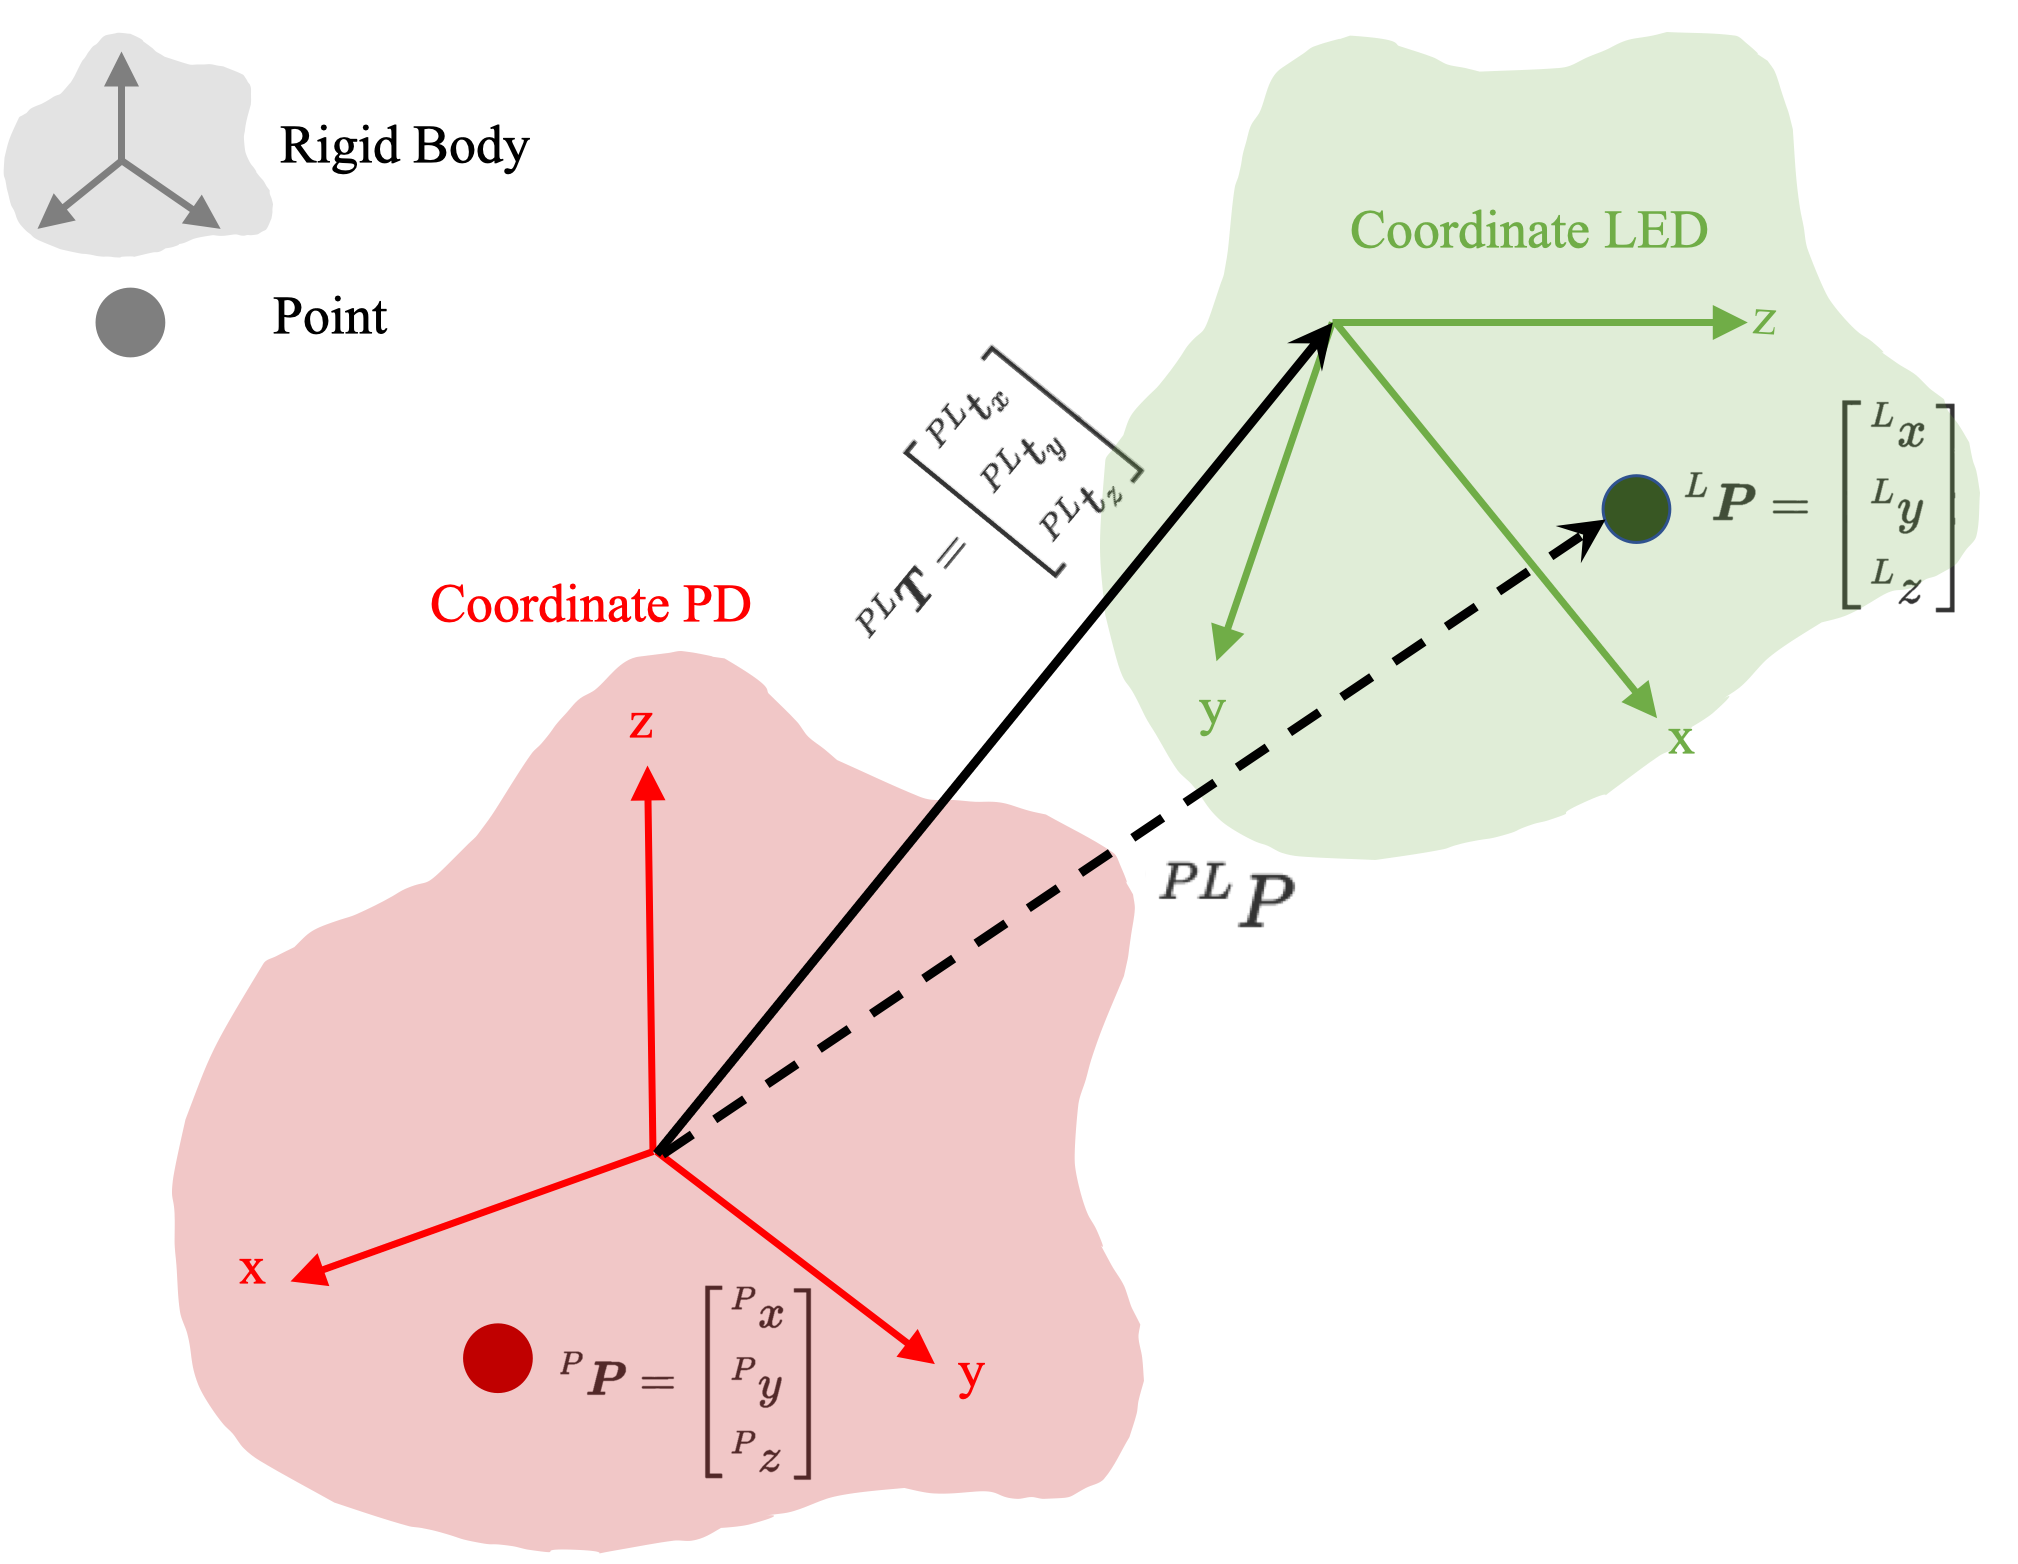
\includegraphics[width=9cm]{ch2pic/homo_trans.png}
        \caption{LED座標系與PD座標系及相對關係}
        \label{pic:homo_trans}
    \end{figure}

    \begin{equation}
        \label{eqn:homogeneous}
        \begin{aligned}
        {\left[\begin{array}{c}
        { }^{P L} P \\
        1
        \end{array}\right]={ }^{P L} \boldsymbol{H}\left[\begin{array}{c}
        { }^{L} P \\
        1
        \end{array}\right] } &=\left[\begin{array}{cc}
        { }^{P L} \boldsymbol{R} \boldsymbol{o} & { }^{P L} \boldsymbol{T} \\
        0 & 1
        \end{array}\right]\left[\begin{array}{c}
        { }^{L} P \\
        1
        \end{array}\right] \\
        &=\left[\begin{array}{cccc}
        { }^{P L} \gamma_{11} & { }^{P L} \gamma_{12} & { }^{P L} \gamma_{13} & { }^{P L} {t}_{x} \\
        { }^{P L} \gamma_{21} & ^{P L } \gamma_{22} & { }^{P L} \gamma_{23} & { }^{P L} {t}_{y} \\
        { }^{P L} \gamma_{31} & ^{P L} \gamma_{32} & { }^{P L} \gamma_{33} & { }^{P L} {t}_{z} \\
        0 & 0 & 0 & 1
        \end{array}\right]\left[\begin{array}{c}
        { }^{L} {x} \\
        { }^{L} {y} \\
        { }^{L} z \\
        1
        \end{array}\right]
        \end{aligned}
    \end{equation}

    % \begin{equation}
    %     ^{PL}\boldsymbol{T}=\left[\begin{array}{l}
    %     ^{PL}x \\ ^{PL}y \\ ^{PL}z
    %     \end{array}\right]
    % \end{equation}

    
    
   其中,兩座標系之間的平移關係$^{PL}\boldsymbol{T}$即為欲得到的相對位置資訊,共有三個自由度。

 



\section{後處理方法分類}
\label{chp:method}
    
    後處理方法可以分成兩部分:室內定位所使用的硬體在接收訊號時,首先會根據量測者所接收的資訊種類有所不同;接收資訊後,如何利用資訊計算出相對位置,則是屬於定位演算法的部分。
    
    

    \subsection{資訊種類}
    
    \begin{figure}[ht]
        \centering
        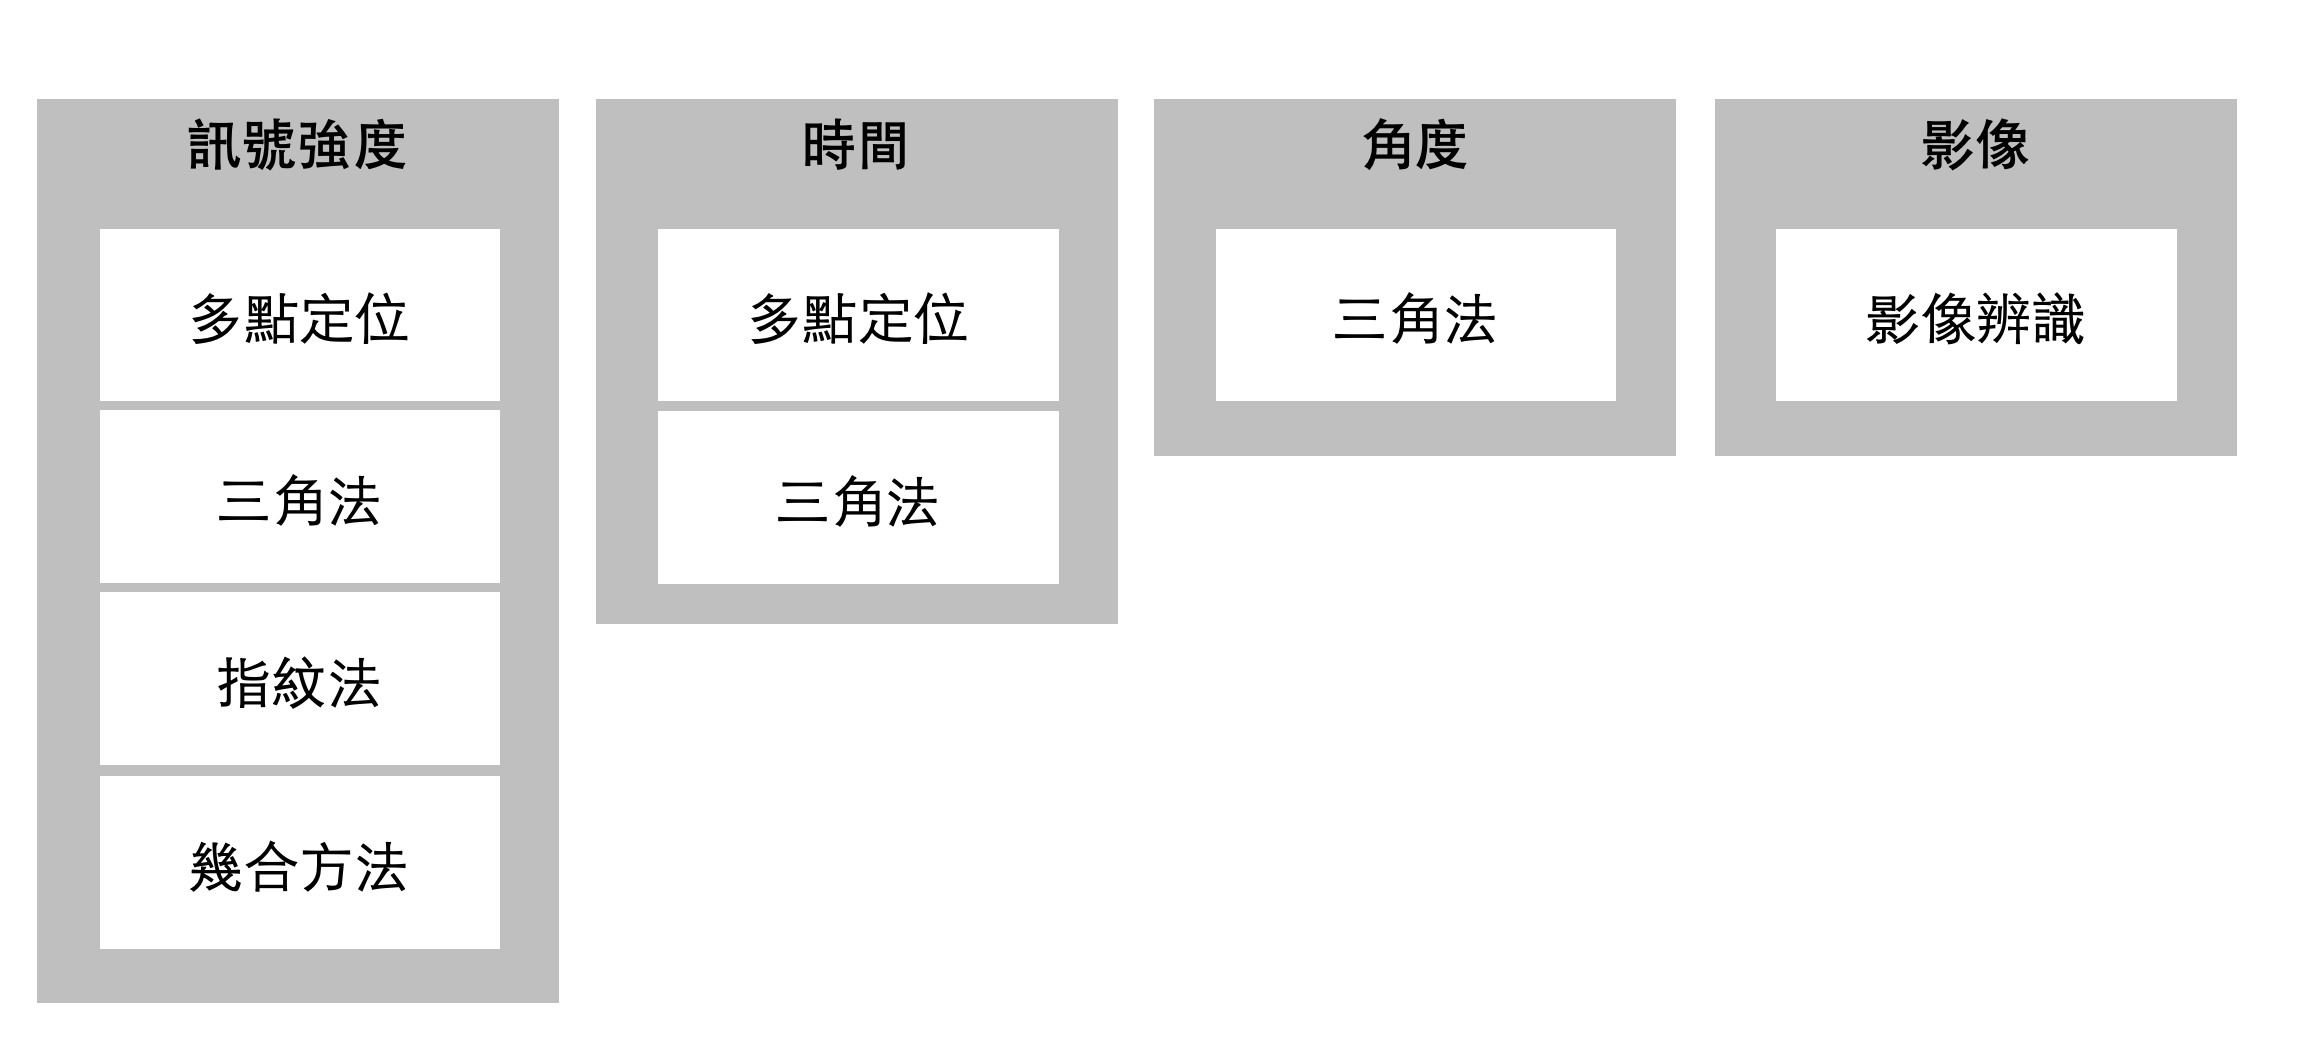
\includegraphics[width=12cm]{ch2pic/method_sort.png}
        \caption{資訊種類與演算法之間的關聯(參考\cite{survey_light2018})}
        \label{pic:method_sort}
    \end{figure}

    訊號強度(Received Signal Strength,簡寫RSS)為最常見的資訊種類,使用的是該硬體所接收到的訊號強度,而利用訊號強度的演算法也十分多樣,包含多點定位、三角法、指紋法等,可參考\ref{chp:method-algorithm}。

    時間資訊種類則是硬體利用訊號之間的時間差,量測距離的方法,常見使用的技術為紅外線,紅外線可以利用訊號傳送到不同接收子的時間差,判斷出之間的距離。若要利用時間資訊,在各硬體之間則需要將時間同步,在實作上為一大挑戰。

    若獲取的是角度資訊,基本上演算法便會搭配三角法,綜合多個接收子的角度獲得相對位置。

    影像則屬於相機獨有,且定位演算法為影像辨識,目標物需有已知的特徵,透過辨識影像中的特徵點,藉由特徵點於影像中呈現的大小、變形,進行計算以回推兩者之間的距離。


    \subsection{定位演算法}
    \label{chp:method-algorithm}
    常見的演算法種類如下:
    \begin{description}
        \item[- 多點定位(Multilateration)] 在環境中建立多個參考點並固定位置,利用目標物與多個參考點的距離,以各參考點為中心、距離為半徑畫圓求交點。
        \begin{figure}[ht]
            \centering
            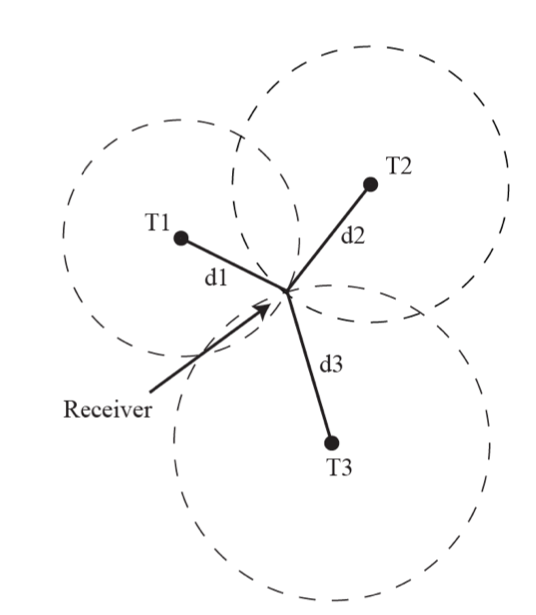
\includegraphics[width=6cm]{ch2pic/multilateration.png}
            \caption{多點定位法\cite{survey_light2020}}
            \label{pic:multilateration}
        \end{figure}
    
        \item[- 三角測量(Triangulation)] 在環境中建立多個參考點,藉由目標物與各參考點之間的角度關係,推算目標物位置。
        \begin{figure}[ht]
            \centering
            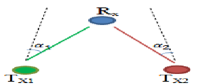
\includegraphics[width=4cm]{ch2pic/triangulation.png}
            \caption{三角測量法\cite{pic:triangulation}}
            \label{pic:triangulation}
        \end{figure}
        \item[- 指紋法(Fingerprinting)] 指紋法在環境中建立多個參考點,在實際進行測量前,需進行事先測量訓練的階段。在訓練階段時需將目標物在環境中移動,蒐集大量訊號數據庫,量測階段則藉由接收訊號與訓練階段所建立的數據庫參照,尋找最有可能存在的位置,近年則是有許多以機器學習方法增加此演算法的精確度。
        \begin{figure}[ht]
            \centering
            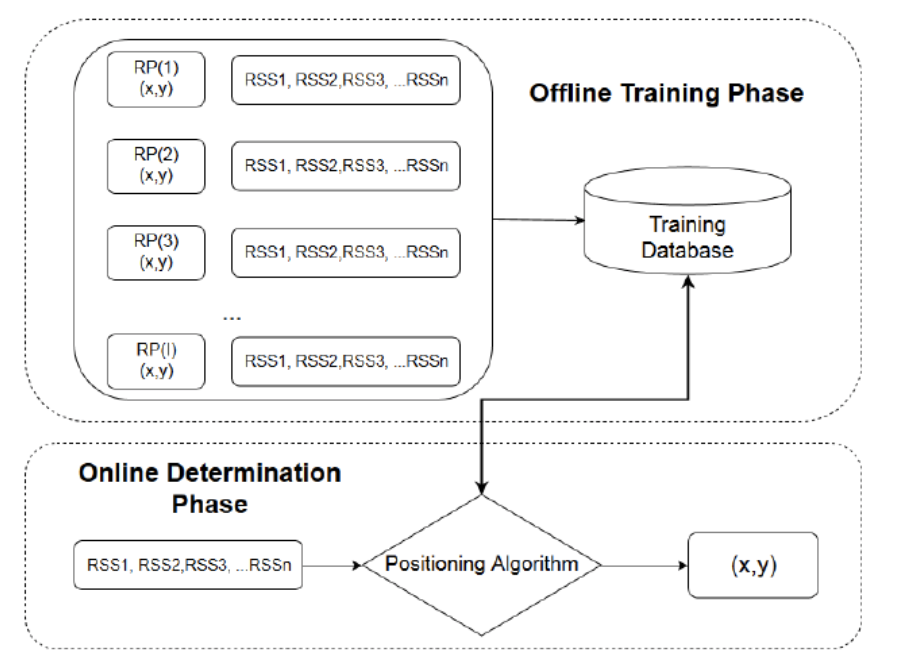
\includegraphics[width=13cm]{ch2pic/fingerprinting.png}
            \caption{指紋法流程圖\cite{pic:fingerprinting}}
            \label{pic:fingerprinting}
        \end{figure}
        \item[- 影像辨識]
        三維空間中的物體,透過相機拍攝成為二維的影像時,為三維空間投影至二維影像平面上的幾何轉換。利用影像辨識求解相對位置時,則是試圖將二維影像中的特徵點比對、轉換回三維空間中,利用PnP演算法(Perspective-n-Point)解出目標物相對相機座標系的位置與方位。
        \begin{figure}[ht]
            \centering
            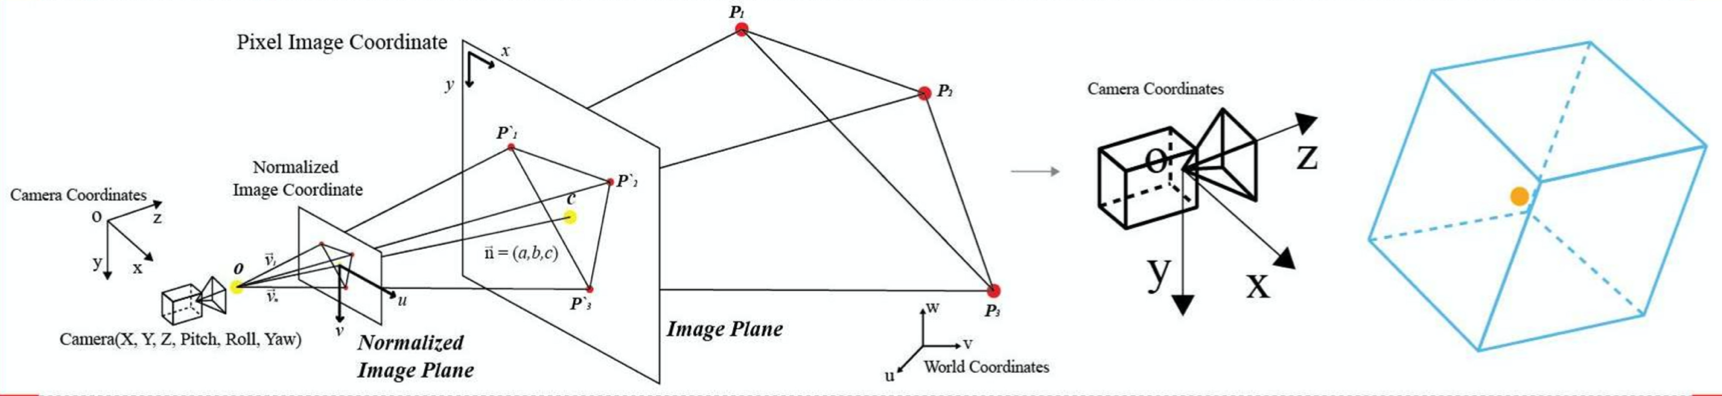
\includegraphics[width=15cm]{ch2pic/image_processing.png}
            \caption{影像辨識示意圖\cite{pic:image_processing}}
            \label{pic:image_processing}
        \end{figure}
        為了使辨識過程中,辨識特徵點的難度降低,通常會設計特徵明顯的標記,例如常見OpenCV中的ArUco標記,利用其快速的辨識ID以及距離、方位等資訊。
        \begin{figure}[ht]
            \centering
            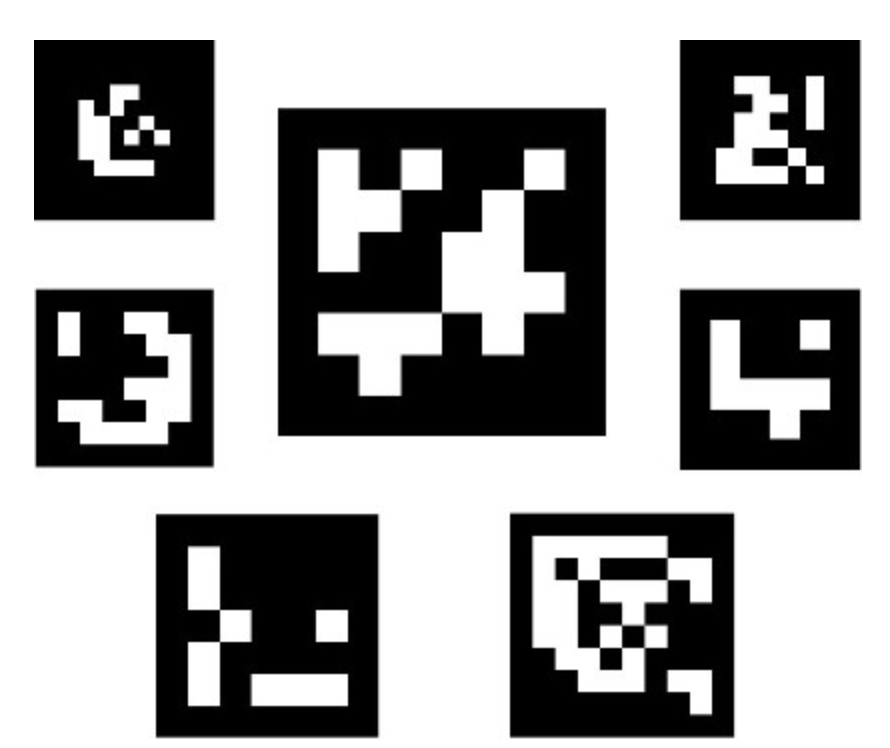
\includegraphics[width=5cm]{ch2pic/aruco.png}
            \caption{ArUco標記例子\cite{pic:aruco}}
            \label{pic:aruco}
        \end{figure}
        \item[- 幾何方法] 
        此類方法常見於LED與PD的定位方法,其接收的訊號強度與距離與角度皆有關,因此需綜合多點定位與三角定位,透過訊號強度與相對位置之間的幾何關係推算相對位置。
    \end{description}

\section{定位技術分類}
\label{chp:technique}
    室內定位所使用的技術(Technique)一樣十分多樣,非電磁波段的定位主要為超聲波,應用訊號發射與接收之間的時間差,推算與目標物之間的距離。然而該技術受溫度影響,且對目標物的辨識能力不佳,因此目前著重在自駕車與載具中障礙物的有無偵測上\cite{survey_ultrasonic},並不符合研究目標,所以以下章節聚焦在電磁波段內的定位進行分析。

    

    \subsection{以電磁波頻率分類定位技術}

        \begin{figure}[ht]
            \centering
            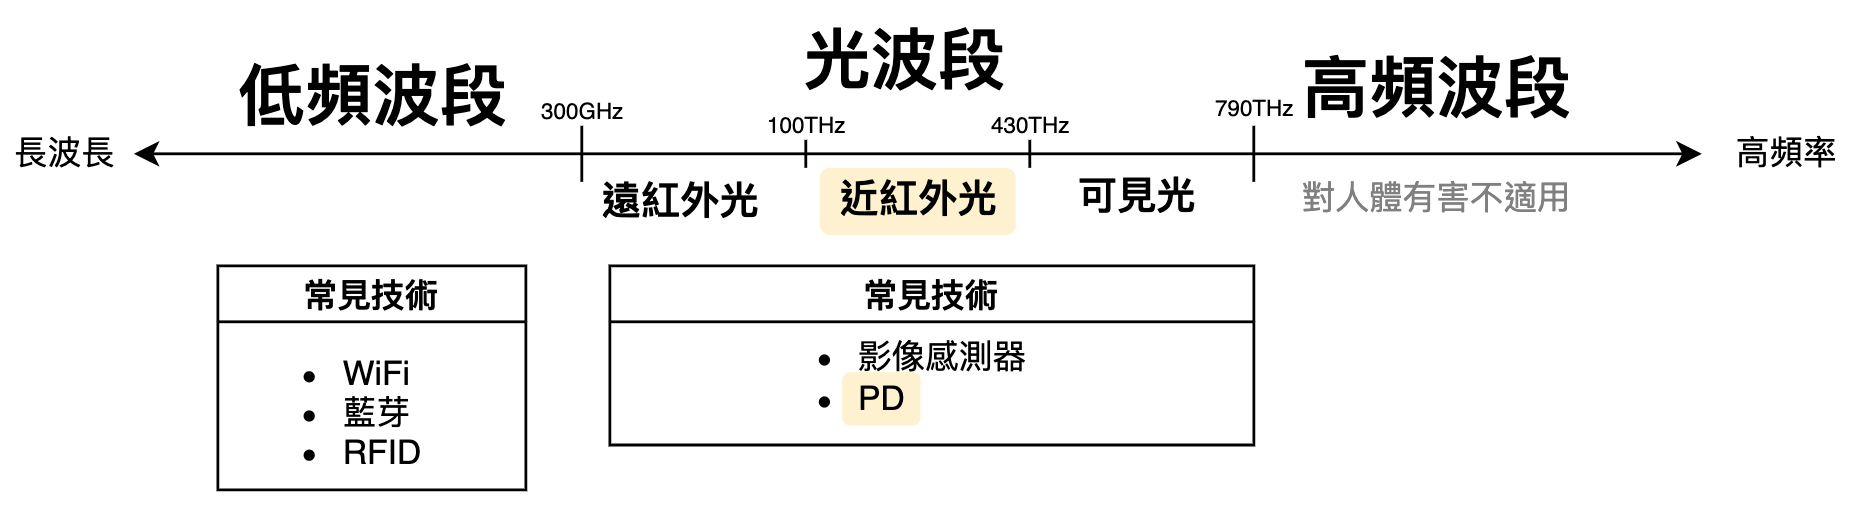
\includegraphics[width=9cm]{ch2pic/technique_sort.png}
            \caption{以電磁波頻率分類定位技術}
            \label{pic:technique_sort}
        \end{figure}

        電磁波段內有許多不同現今受到關注的量測技術,電磁波段內常見的技術於\ref{chp:intro}內有簡單介紹,而電磁波以光速傳播,擁有高傳播速度與不受介質溫度與濕度影響的特性,減少可能對量測訊號造成影響的因素。

        本段落由電磁波的頻率切入進行分類,頻譜圖如圖\ref{pic:spectrum},大致分為兩部分探討:\ref{chp:radio}探討頻率低於300GHz的低頻波段\cite{book_electromagnetic},其中包含Wifi、藍芽、RFID;\ref{chp:light}介紹另一類:頻率介於790THz與300GHz之間的光波段,包含紅外線、可見光定位以及相機定位。至於頻率高於790THz的高能量波段不加以考慮,原因是電磁波頻率越高所含能量越高,此特性使得高頻波段(X光、紫外線、伽瑪射線)對人體有害,因此無法使用於定位。

        \begin{figure}[ht]
            \centering
            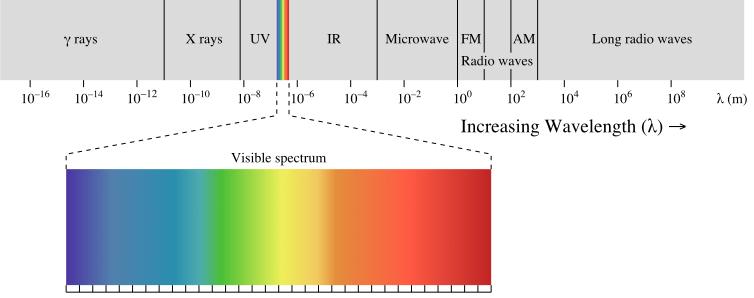
\includegraphics[width=9cm]{ch2pic/electro_spectrum.png}
            \caption{電磁波頻譜度\cite{Spectrum}}
            \label{pic:spectrum}
        \end{figure}

        \subsubsection{無線電波段定位}
        \label{chp:radio}
        
            低頻波段也就是俗稱的無線電波(Radio Waves),應用發展歷史長,對於可使用的頻率有嚴格規範,台灣由國家通訊委員會訂定嚴格的可使用頻率波段\cite{rf_law},保證軍警、醫療、廣播等的傳播需求。常見的定位技術包含室內與多數裝置既有的WiFi與藍芽裝置,或是較新的RFID定位技術。
        
            無線電波的主要特色包含可穿透大多障礙物,可用於跨房間非可視範圍(NLoS)的定位\cite{survey_indoor2018},增加了應用場域,然而也大大提升了訊號處理的難度,感測器難以辨別訊號衰減原因為距離、角度、亦或是障礙物,因此選擇非可視範圍內定位即捨棄精度。除此之外,無線電波的傳遞距離很長,定位範圍較廣。所需面對的誤差處理包含電磁干擾、同頻道干擾(Co-channel Interference)、受障礙物與金屬影響的穿透較果等。

            大多無線電波段的定位系統皆是利用指紋法、多點定位、三角法的方式,共通點是都需要多個參考點,事先的安裝複雜,應用場域著重在固定場域,而精度多為公尺量級。
        
            舉RFID定位來說,大多應用在固定的場域中建立數據庫,或是利用大量的感測器與訊號發射器來判斷定位\cite{survey_rfid}。

            \begin{figure}[ht]
                \centering
                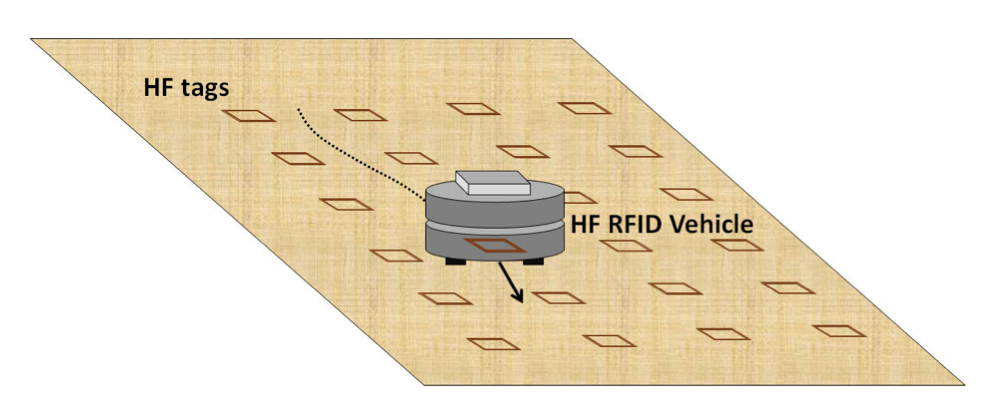
\includegraphics[width=5cm]{ch2pic/rfid_system.png}
                \caption{RFID定位系統示意\cite{survey_rfid}}
                \label{pic:rfid_system}
            \end{figure}

        % 補系統圖


        \subsubsection{光波段定位}
        \label{chp:light}
            光波段的定位發展近幾年來十分顯著,主要原因為光學硬體上的進步,促使光通訊(LC, Light Communication)的發展,使發光與感光元件具有傳播ID、訊息等資訊的能力,因此光通訊與光定位便於近年得到研究關注。在如今電磁波訊號充斥環境的狀況下,光波段提供一替代方案,除了可以應用在禁用電磁波的機場與醫療場域,其特性還包含較高的頻寬。
            
            
            再來,光波段無法穿透障礙物,僅能進行可視範圍內(LoS)的定位,捨棄廣域的定位,獲得較為單純的量測數據。此特性同時增加光通訊的安全性以及穩定度,著重針對可視範圍進行通訊與定位,不必考量其他訊號。例如載具運行時,僅需著重分析於身旁的其他物體,位於隔壁房間的物體毫不重要,此時該特性即可忽略不重要的資訊,增加處理速度與有用訊號穩定度。


            電磁波另一個特性為:波長愈短可達到的量測精度愈高,且感測器與訊號發射器的硬體大小也愈小,例如市售便宜常見的光波段感測器如PD感光二極體尺寸量級為mm或以下\cite{datasheet:led_sfh4545}且能耗低,而使用低頻波段的RFID感測器常見量級為cm\cite{datasheet:rfid_tag}。


    \subsubsection{小結}

        
        
        綜上所述,比較低頻波段與光波段,從精度層面來看,光波段捨棄非可視範圍的定位以減少影響訊號的因素,加上波長較短的特性,精度較高,較符合本研究目標;針對靈活應用的需求,光波段無論是小體積還是低能耗、靈活度,都是較佳的選擇,且並不受限於機場與醫療場所的應用。因此,根據本研究目標所需,將研究方法聚焦在光波段的定位上。

        \begin{figure}[ht]
            \centering
            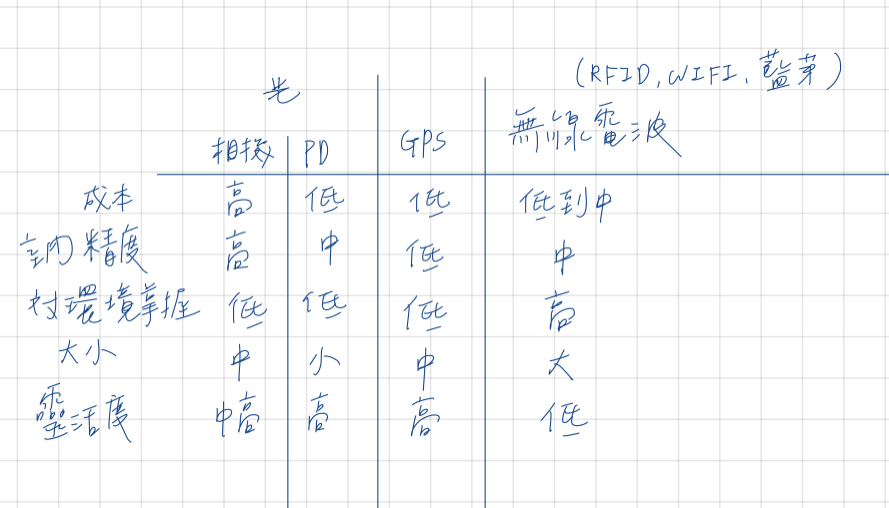
\includegraphics[width=10cm]{ch2pic/method_compare.jpg}
            \caption{定位方法特性}
            \label{pic:method_compare}
        \end{figure}

    \subsection{光波段定位的分類}

        

        光波段的分類可從兩方向切入:使用波段與感測器硬體選擇,以下依序進行探討:

        \subsubsection{使用波段選擇:可見光或紅外光}

        \begin{description}
        \item[- 研究普及度]\hfill 

        首先,現今室內定位的研究主要著重在可見光的部分\cite{survey_light2018},搭配著室內環境都具有的光源,其優點強調在不對室內環境進行過多改動上即可進行定位量測。然而本研究需能靈活將光源安裝於任意被觀察物上,因此室內充足的可見光光源並不能成為訊號載體,因此雖然可見光波段擁有較多文獻與研究,其並不符合本研究目標,僅能參考方法與眼算法等,所以挑選光波段重點將著重在降低誤差上。

        \item[- 硬體技術] \hfill 
        
        光波段的光感測器常見的材料有矽(Si)、鍺(Ge)與III或V族元素,價格最便宜的是矽材料,而矽感測器的感光波段約在400-1000nm,也就是可見光與近紅外光(NIR)波段。這也是為什麼普遍對紅外光波段的硬體都有價格昂貴的印象,但凡波長較長的紅外光在硬體材料便需要使用到昂貴的鍺或其他三五族元素\cite{si_pd}。因此,考量到硬體的價格與普遍性,無論是PD還是影像感測器,挑選可見光與近紅外光波段較為合適。

%_________________________________________

        \item[- 誤差] \hfill 
        

        光波段的誤差來源主要包含多重路徑傳輸(Multipath effect)與環境光源(Ambious Light Source)\cite{survey_light2020},其中環境光強度過高可造成訊號偏移甚至硬體飽和導致訊號失真,因此需有效的降低環境光源的強度以保持定位的準確度。環境光源包含了室內的光源以及太陽光源,室內的光源使用交流電的頻率約在120hz,可以針對頻率進行濾波,而太陽光源的強度則隨頻率增減。從太陽光頻譜圖可以觀察到,太陽光於光波段受到大氣層吸收有三處的能量較低,藉由挑選低谷頻率,即可有效降低太陽光對系統的影響。

        利用光波段定位最大的困難就是要克服其他光所造成的雜訊(Shot Noise),因此在選擇工作波長時,挑選自然環境中強度較低的波段。日常環境中的光源包含太陽光與燈,太陽光可以從圖\ref{pic:solar_spectrum}太陽輻射波譜(Solar Irradiance Spectrum)觀察強度與波長的關係,低谷出現在760nm左右的氧氣吸收帶(Oxygen A-band)、與940nm和1550nm附近被水蒸氣吸收之波段\cite{book:solar_spectrum}。

        \begin{figure}[ht]
            \centering
            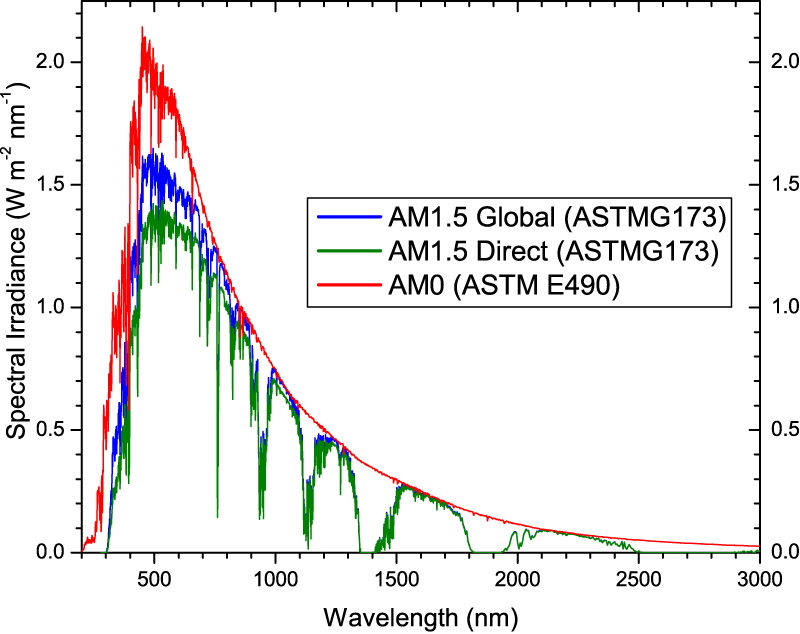
\includegraphics[width=10cm]{ch2pic/solar_spectra.png}
            \caption{太陽輻射波譜\cite{astm}}
            \label{pic:solar_spectrum}
        \end{figure}

        

        \begin{figure}[ht]
            \centering
            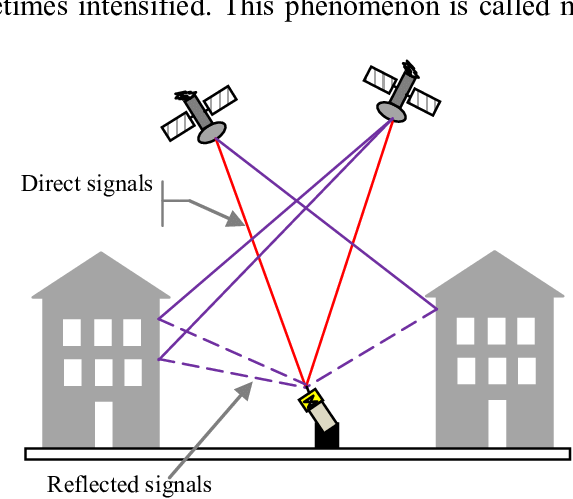
\includegraphics[width=6cm]{ch2pic/multipath.png}
            \caption{多重路徑傳輸\cite{pic:multipath}}
            \label{pic:multipath}
        \end{figure}

        \item[- 對人眼影響]\hfill 

        本研究目標需應用於移動物體上,因此紅外光呈現優勢,即使光源在環境中的使用者面前直射,紅外光無法在視網膜成像的特性讓使用者並不會感受到影響;反之,朝人眼照射可見光源會造成干擾。除此之外,紅外光頻率低、能量較小,且於視網膜成像的難度也大,因此較為安全。

        \end{description}


        

        \subsubsection{硬體選擇:PD或影像感測器}

            PD僅能感測到強度資訊,而強度資訊受LED出射角度、PD入射角度、距離影響,變數多使得獲得相對定位資訊難度高,然而其有極高的取樣頻率,可高達千赫茲甚至萬赫茲,高取樣頻率在光通訊上能夠較好的進行編碼與解碼,且硬體成本相較影像感測器來說非常低。

            影像感測器就是常見的相機,每次取樣會獲得多個像素的強度資訊,獲取的資訊量極多,其定位方式是利用辨識已知的特徵圖案的大小與變形,推算目標物的距離以及姿態,其中若量測範圍要廣,則特徵圖案則需要越大越好,常見的Aruco標誌尺寸建議在16公分以上。然而其取樣頻率大多在百赫茲內,且視覺辨識所需要的運算資源多,不僅成本高,運算速度也較慢。

            %補


        \subsubsection{小節}
        
        
        % [可做一張十字圖:(相機vsPD)(可見光vs紅外光)]

        權衡之下,挑選於太陽光輻射光譜中低谷的760nm與940nm波段,並選擇使用PD作為接收子,能夠同時享有硬體選擇多且價格低的優勢,又減少了太陽光源所影響的程度,並使裝置保持輕巧低成本又不干擾人眼與日常生活的優點。選擇使用的硬體技術後,接著於\ref{chp:LEDandPD}介紹該技術如何進行定位計算。


\section{LED與PD的定位方法}
\label{chp:LEDandPD}
    我們將定位方法聚焦在LED與PD的定位方式,而此種系統是將單個或多個LED安裝在目標物上,各LED藉由編碼來區別各自的訊號,而PD安裝於觀察物上,將每個PD所接收的訊號分別解碼,得到各LED的訊號強度。

    \begin{figure}[ht]
        \centering
        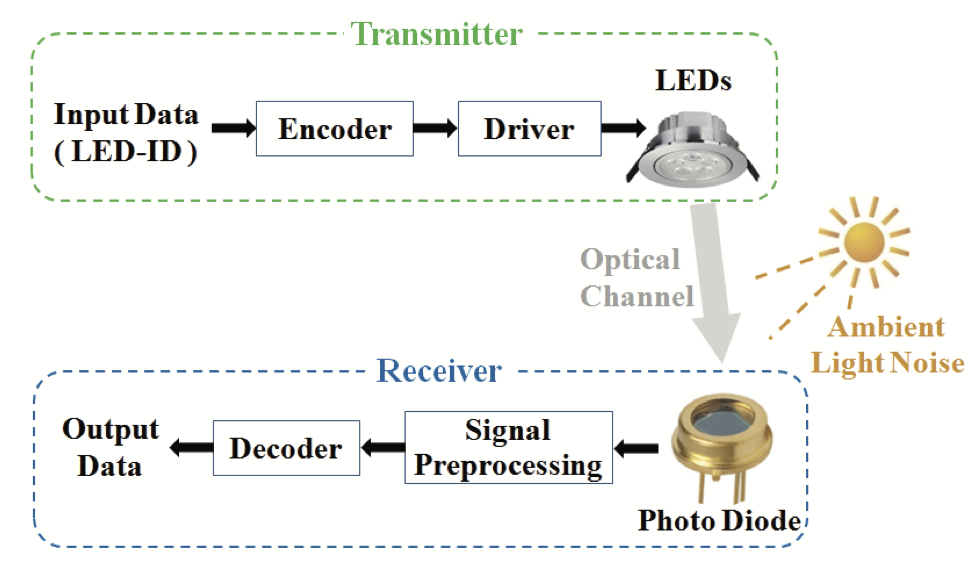
\includegraphics[width=6cm]{ch2pic/vlc.png}
        \caption{LED與PD定位系統架構\cite{decoding}}
        \label{pic:vlc}
    \end{figure}

    為深入了解系統運作方式,從基本的光領域常用單位介紹;有基本了解後,開始介紹LED與PD的硬體特性與參數,以及光傳播上的模擬建模,再進入系統整體的細節,以及此領域的文獻探討。

    \subsection{光學常用單位介紹}
        
        由於光領域所使用的單位與機械領域差距較大,進入PD與LED定位的探討之前,先對光領域的一些術語與單位進行介紹。

        首先,描述光照的單位在文獻上經常有些混亂,單位分為兩種制度,且常有混用以及口語省略,令人感到困惑,因此以下進行釐清:光領域中的計量單位大致分成兩種系統,輻射測量學(Radiometry)與光度測量學(Photometry),兩領域以不同單位描述光源,其中輻射測量學著重在電磁波輻射的量測,描述通量單位為瓦特(Watt);而光度測量學著重在人演可見之可見光波段的研究,通量單位為流明(Lumen),同樣物理量下單位定義不同。\cite{radiometry_and_photometry}
        

        \begin{figure}[ht]
            \centering
            \caption{輻射測量學與光度測量學的物理量}
            \label{tab:photometry}
            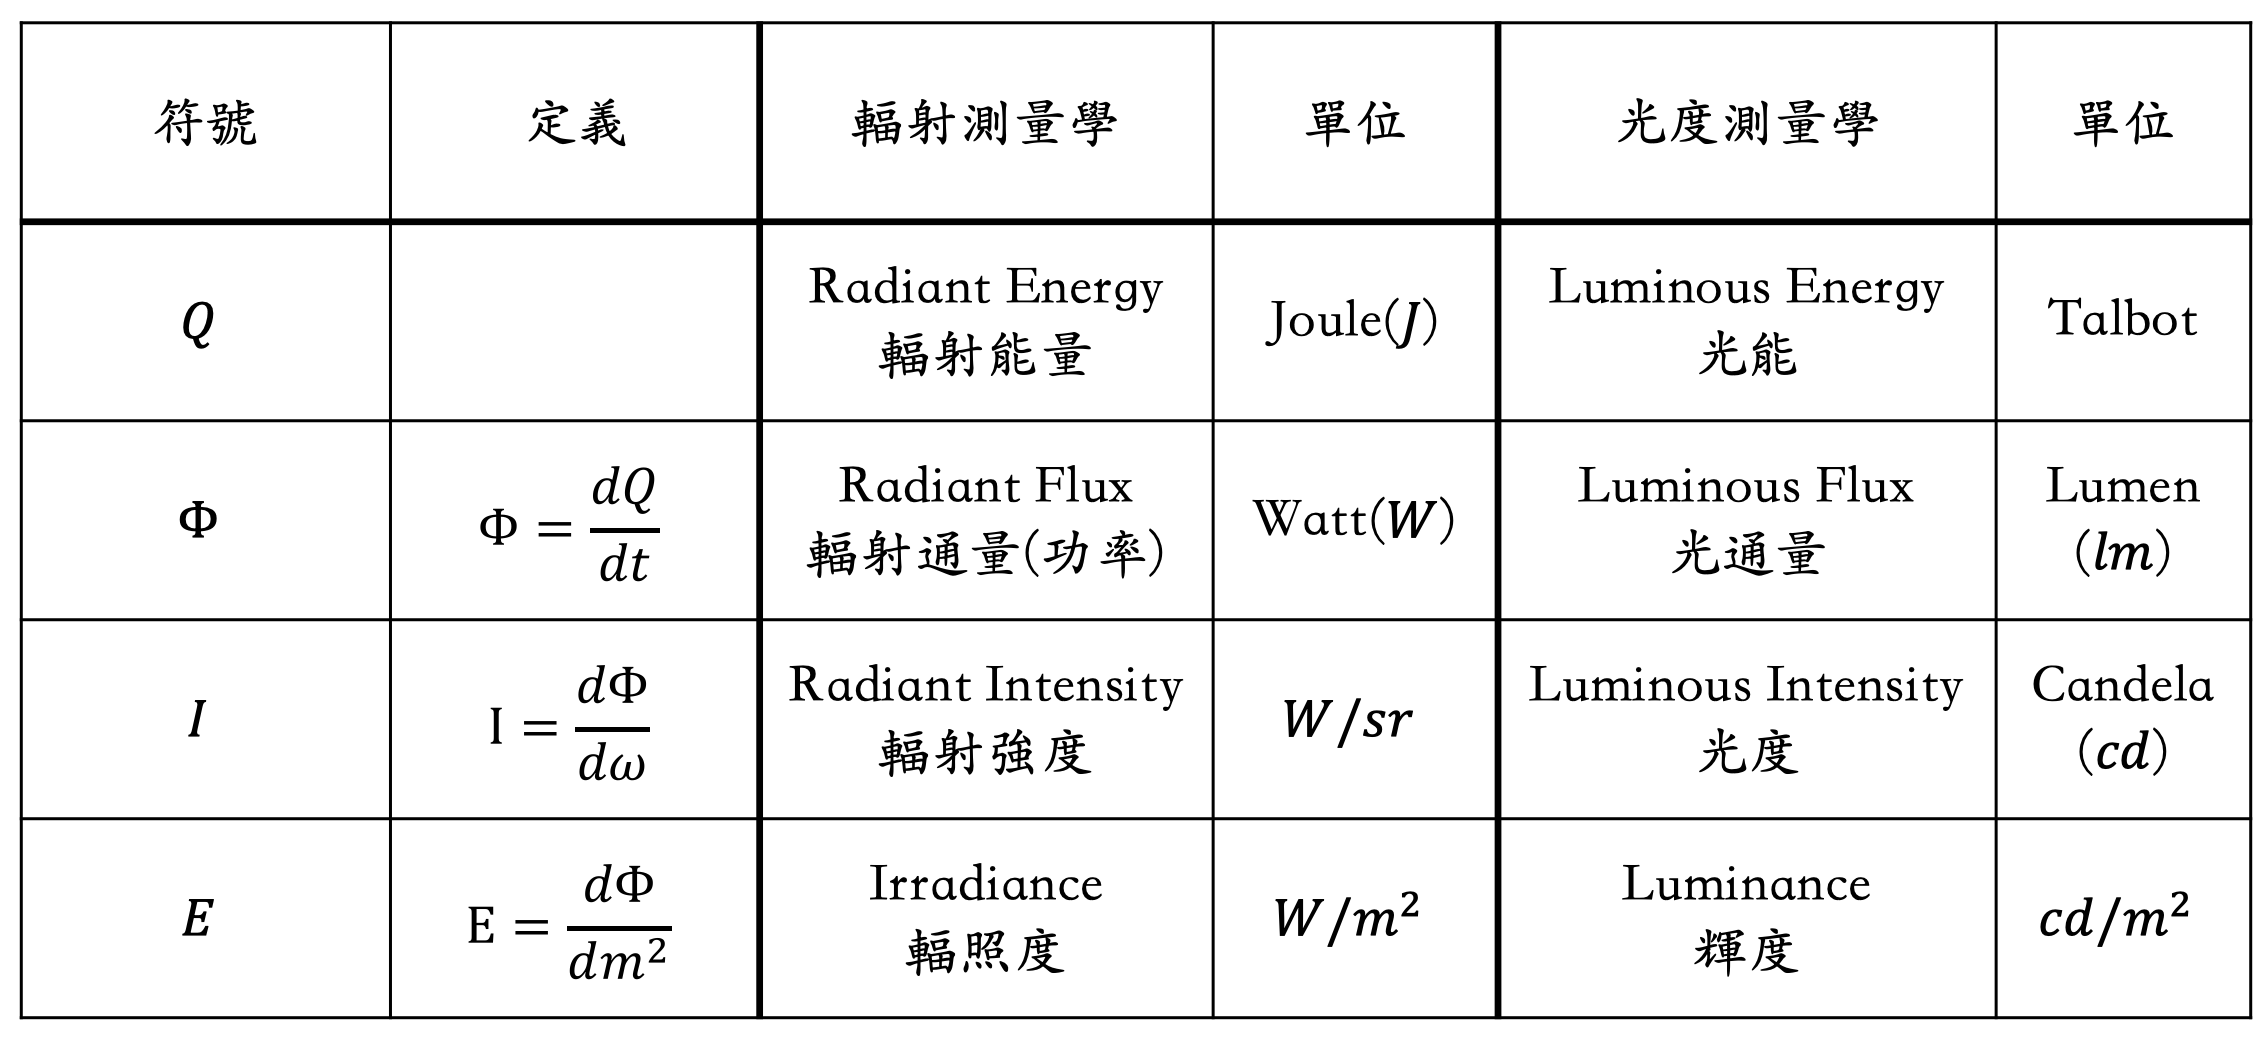
\includegraphics[width=10cm]{ch2pic/photometry_table.png}
        \end{figure}


        本研究聚焦在近紅外光波段,因此本論文所使用的單位系統為輻射測量學的系統,然而文獻上可見光定位數量較多,因此在單位的換算上需特別注意,以下針對光領域常用物理量簡單敘述。

        
        \begin{description}
            \item[- 立體角 Solid Angle $\Omega$] \hfill
                
                描述二維空間中的角度單位為弧度,表示夾角內的弧長與半徑比例,而單位弧度的定義是半徑與圓弧長度相等時的圓心角。
                然而光源存在於立體空間中,而空間中描述角度的物理量即為立體角(Solid Angle),該物理量代表錐狀立體角在球面上的表面積與半徑平方的比例,其中,單位為球面度(steradians, 簡寫$sr$)代表在半徑為$r$的球體中,立體角投射出的表面積為$r^2$。

                \begin{figure}[ht]
                    \centering
                    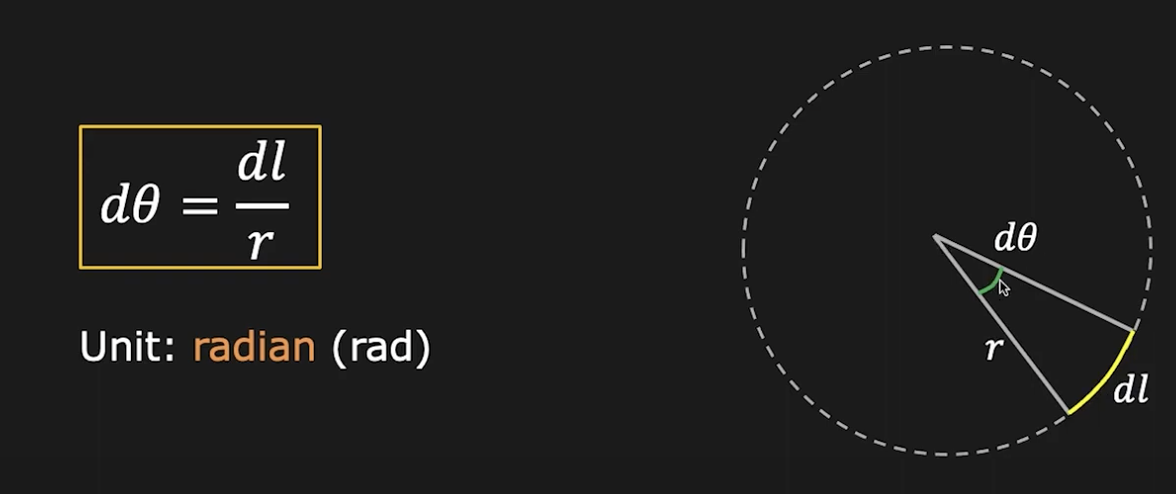
\includegraphics[width=5cm]{00temppic/1.png}
                    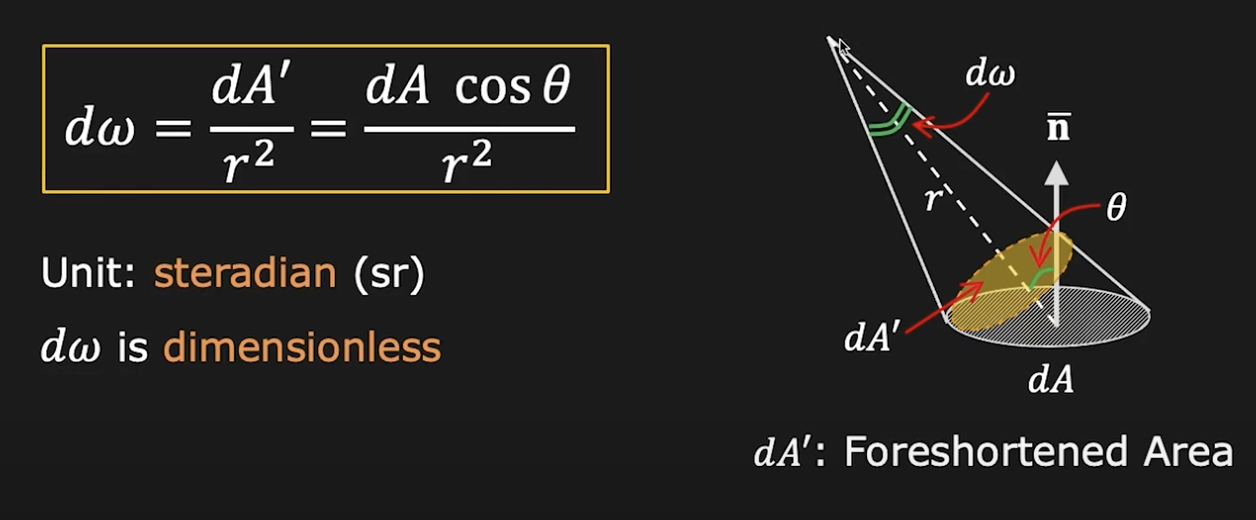
\includegraphics[width=5cm]{00temppic/2.png}
                    % \caption{多重路徑傳輸\cite{pic:multipath}}
                    % \label{pic:multipath}
                \end{figure}

            \item[- 輻射通量 Radiant Flux $\Phi$]  \hfill
                
                描述光照功率的物理量為通量(Flux)或稱輻射功率(Power),代表每單位時間的輻射能量,單位為瓦特,而大多LED規格表上以此物理量來描述LED在指定電流下可產生的最大光功率。

                \begin{figure}[ht]
                    \centering
                    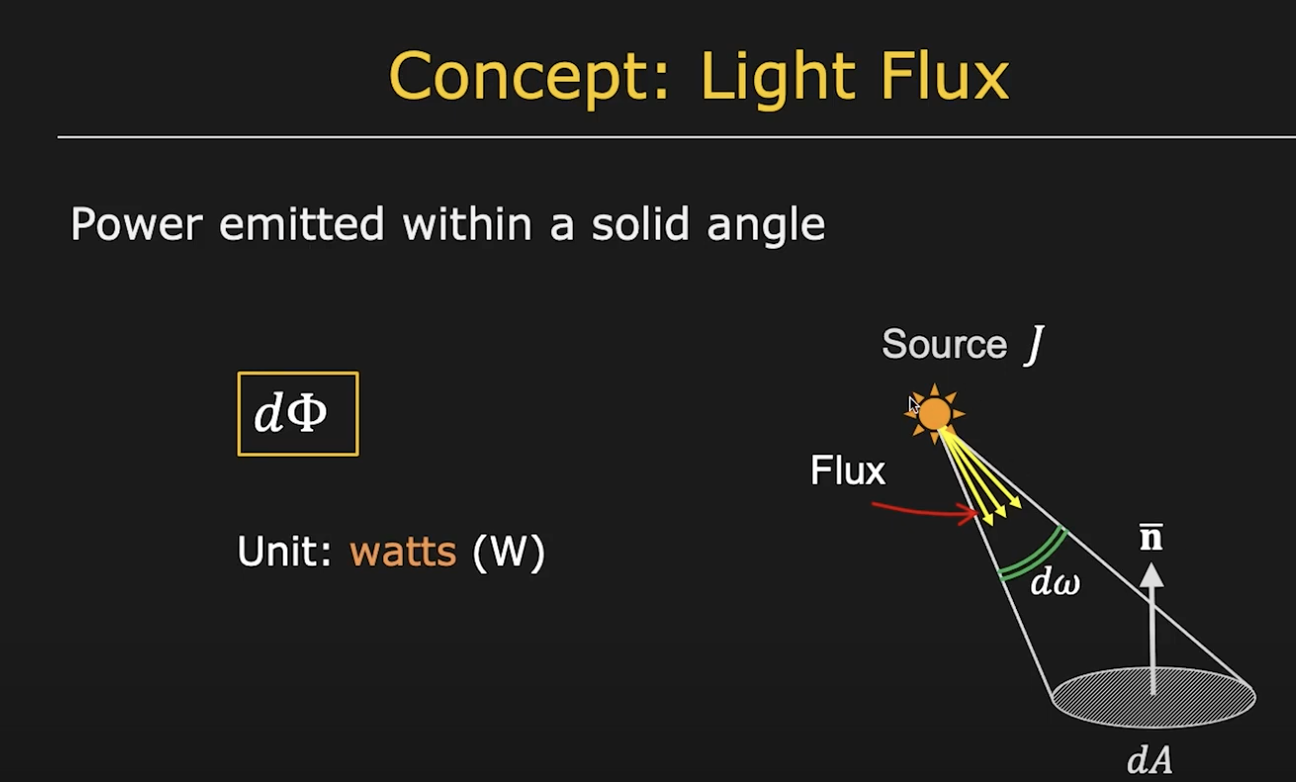
\includegraphics[width=5cm]{00temppic/3.png}
                    % \caption{多重路徑傳輸\cite{pic:multipath}}
                    % \label{pic:multipath}
                \end{figure}

            \item[- 輻射強度 Radiation Intensity $I$] \hfill
             
                每單位立體角所含的通量稱為輻射強度,此物理量常用於描述光與角度之關係,其與距離無關。
                \begin{figure}[ht]
                    \centering
                    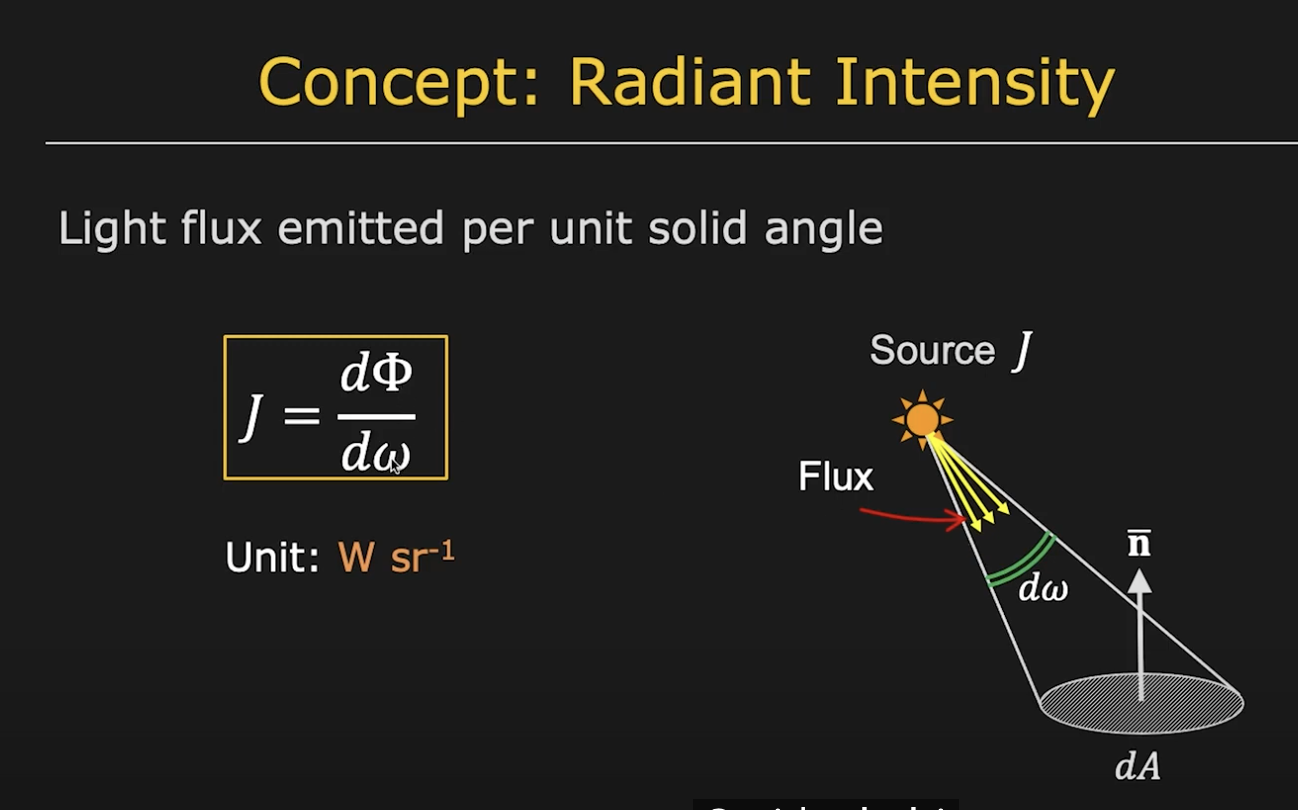
\includegraphics[width=5cm]{00temppic/4.png}
                    % \caption{多重路徑傳輸\cite{pic:multipath}}
                    % \label{pic:multipath}
                \end{figure}

            \item[- 輻照度 Irradiance $E$] \hfill
                \begin{figure}[ht]
                    \centering
                    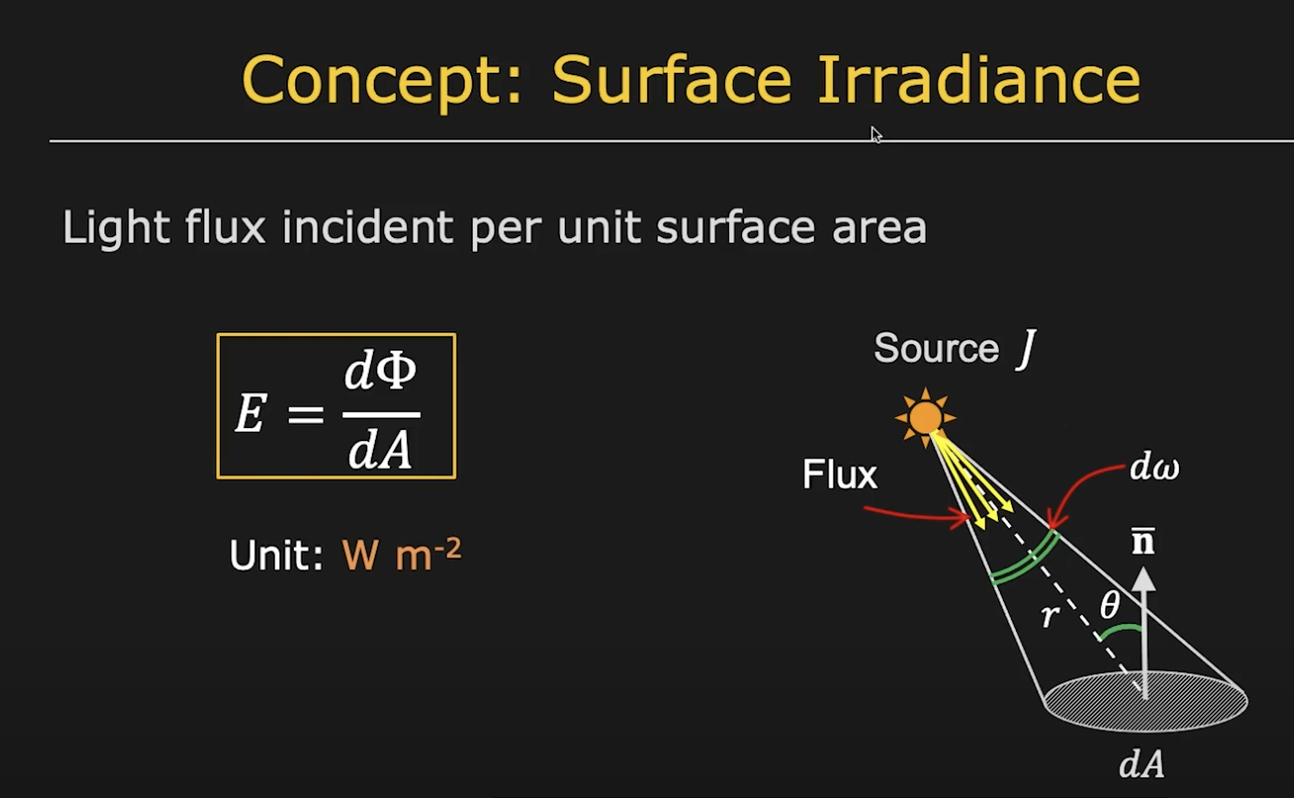
\includegraphics[width=5cm]{00temppic/5.png}
                    % \caption{多重路徑傳輸\cite{pic:multipath}}
                    % \label{pic:multipath}
                \end{figure}
                每單位面積所含的通量稱為輻照度,其中照射面積隨著距離$D$增加而平方遞增,在已知距離的情況下,即可利用立體角的定義,換算輻射強度與輻照度之間的關係\ref{eqn:I2E},$\omega$為入射表面與光源之夾角。
                
                \begin{equation}
                    \label{eqn:I2E}
                    E=I\cos\omega/D^2
                \end{equation}

                
             
        \end{description}

        

        

    \subsection{LED與PD的硬體參數與特性}

    LED與PD硬體有許多種類,最常見的市面上LED與PD為軸對稱並滿足朗博輻射模式(Lambertian Radiation Pattern),本論文僅考慮此類硬體。軸對稱代表當LED或PD僅對出射角或入射角以及距離有敏感度,以球座標系來看,凡在同一仰角與距離,無論方位角為何,光照強度與感光強度皆相同。

    
        

        \subsubsection{擺放自由度}

        LED與PD量測系統包含許多參數,其中針對各LED與PD如何擺放,則可以藉由設計電路板、設計載體與擺放方式,在硬體購入後仍有改變的空間。而在描述座標系空間中的LED與PD時,一共有五個自由度,包含擺放位置$P$的三個分量$x,y,z$,以及定義指向的單位向量$N$。由於LED與PD皆為軸對稱,因此僅有兩個自由度:仰角$\alpha$與方位角$\beta$,$N$在卡氏座標系下的xyz分量則為$u,v,w$。

        %補公式

        \begin{figure}[ht]
            \centering
            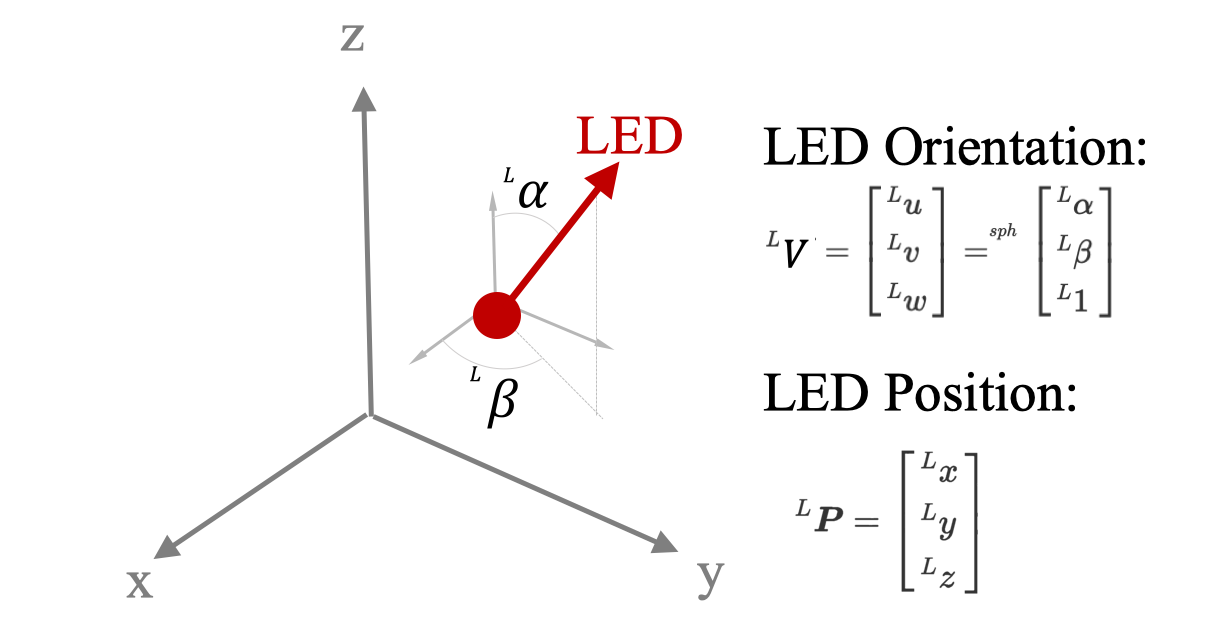
\includegraphics[width=10cm]{ch2pic/LED_config.png}
            \caption{LED在座標系中的擺放自由度}
            \label{pic:led_config}
        \end{figure}


        \subsubsection{硬體參數}

        系統中,其他參數與硬體設計相關,在購置後便不能改變,此類稱為硬體參數,包含了影響模式(Pattern)與影響發光或接收強度的參數。

        \begin{figure}[ht]
            \caption{LED與PD對模式與強度影響之硬體參數}
            \label{tab:hardwarepara}
            \centering
            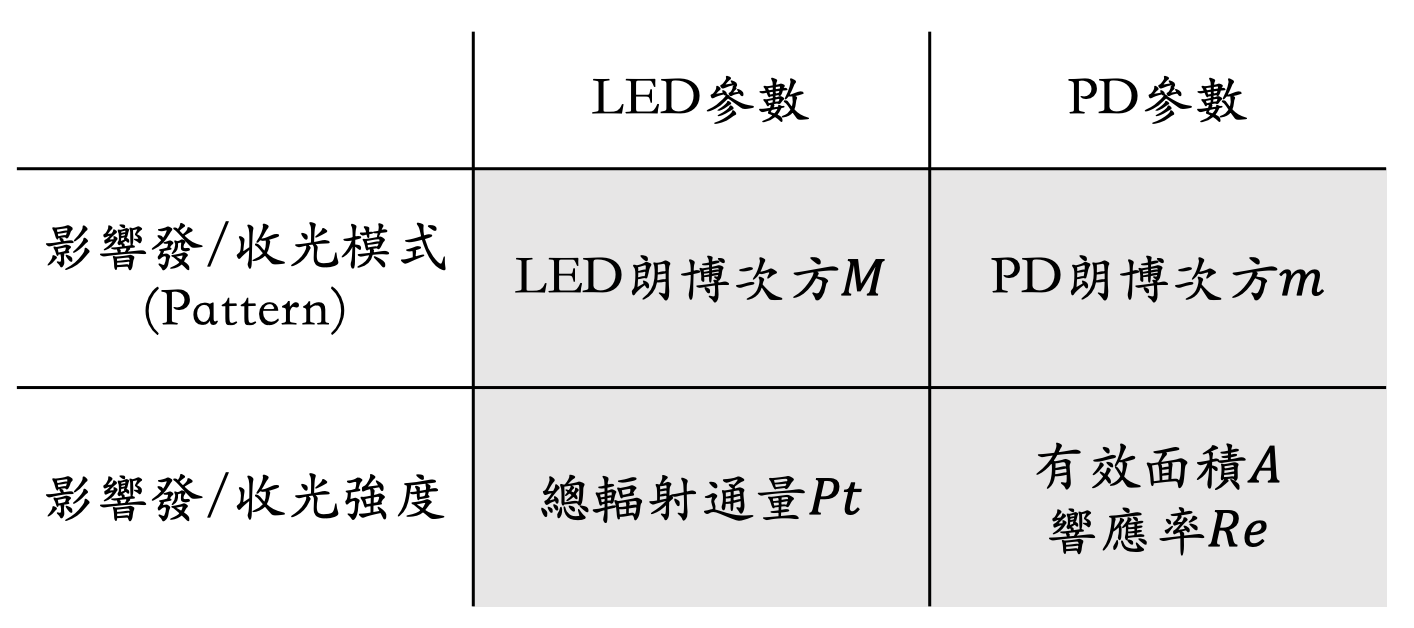
\includegraphics[width=6cm]{ch2pic/tab_hardwarepara.png}
        \end{figure}


        \ref{eqn:model}描述LED輻射強度傳遞到PD接收的輻射強度之間的轉換,單位雖然是輻射強度,然而PD硬體輸出的物理量是電流$Ie$,之間的轉換受到PD的響應率和飽和上限$s$影響。


        \begin{equation}
            \label{eqn:current}
            Ie = \begin{cases}\Phi\times Re, & \text { if } Ie<s \\ s, & \text { otherwise }\end{cases}
        \end{equation}

        \subsubsection{朗博輻射模式}

        LED與PD的照射與接收模式(Pattern)可以用朗博輻射模式(Lambertian Radiation Pattern)量化,代表感光與發光強度隨著LED出射角與PD入射角的增加而變小,其衰減模式可用餘弦函數(cosine)的M次方(power)表示,M代表的是朗博次方(Lambertian Order)。

        \begin{equation}
            \label{eqn:lambertian_pattern}
            I(\omega)=I(\omega=0)\times\cos(\omega)^{M}\\
        \end{equation}

        以二維的角度來看如圖,LED光照射的能量隨出射角度增加而減少,在LED中心軸的方向強度最高,在此描述LED強度時不考慮距離。如先前所述,LED為軸對稱,因此三維的照射模式即為二維模式以中心軸旋轉。在同樣出射角下,光輻射強度相同。
        
        

        以較直觀的方式來解釋朗博次方,其主要是在敏感度與照射範圍中的取捨:朗博次方較小時,其照射範圍較大,最大可以覆蓋接近半個球面,光強度隨出射角度衰減的速度不大,也就是對不同入射角度的敏感度則不高。反之,朗博次方較大的硬體雖然覆蓋範圍較小,但對覆蓋範圍內的角度變化敏感度高。如圖\ref{pic:lambertian},不同朗博次方的PD在接收模式就呈現不同的特性,在此特別注意接收模式僅與角度有關。

        \begin{figure}[ht]
            \centering
            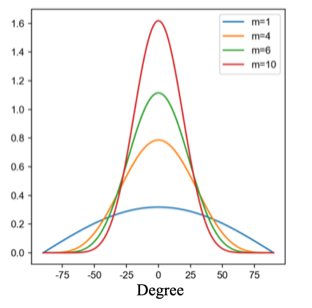
\includegraphics[width=6cm]{ch2pic/lambertian.png}
            \caption{朗博次方與輻射模式}
            \label{pic:lambertian}
        \end{figure}

        

    \subsection{光傳遞模型}

    光傳遞模型中,除了硬體參數以外,受到三個參數影響:距離$D$、PD入射角$\phi$、LED出射角$\theta$,其中出入射角如圖\ref{pic:interactive},分別為硬體中心軸與距離向量之間的夾角。

    \begin{figure}[ht]
        \centering
        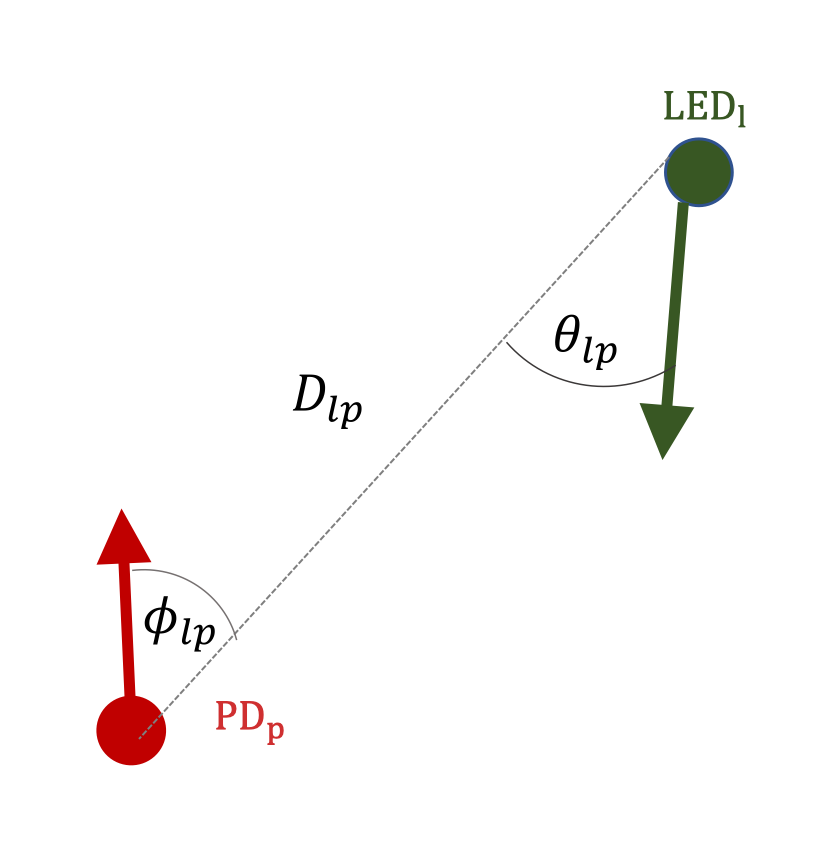
\includegraphics[width=6cm]{00temppic/7.png}
        \caption{LED與PD的交互關係}
        \label{pic:interactive}
    \end{figure}

    從LED發光開始分析,\ref{eqn:lambertian_pattern}描述了光輻射強度$I$在不同入射角的關係,將整個半球中的輻射強度積分,得到LED在整個半球上所照射的總瓦數比例,將該值倒數,即可由LED發射之總能量推算各入射角的光輻射強度,\ref{eqn:lambertian}完整描述LED的發光輻射強度。
    
    \begin{equation}
        \label{eqn:lambertian}
        I(\omega)=Pt\frac{(M+1)}{2 \pi} \cos \omega^{M}
    \end{equation}
    
    空間中光波由LED傳遞至PD的部分以式\ref{eqn:model_pre}描述,藉由\ref{eqn:I2E}將距離對照射範圍的影響考慮進去,,其中PD的接收範圍由硬體參數有效面積$A$描述,藉由乘上有效面積則可將單位轉換回輻射強度。透過朗博次方描述PD接收模式,即可完整的描述從LED到PD的光傳遞模型。
    
    \begin{equation}
        \label{eqn:model_pre}
        \Phi=I\times\frac{ 1 }{D^2}\times A\times\cos\phi^{m} \\
    \end{equation}
    


    本論文為多LED對多PD的系統,在描述第$p$個LED量測到第$l$個LED的強度$\Phi_{lp}$時,以下標備註,完整公式可由\ref{eqn:model}描述。
    
    \begin{equation}
        \label{eqn:model}
        \Phi_{lp}=\frac{ A_p\cos\phi_{lp}^{m_{p}} }{D^2_{lp}}\times Pt_l\frac{(M_{l}+1)}{2 \pi} \cos \theta_{lp}^{M_{l}}  \\
        =k_{lp}\frac{{\cos\theta_{lp}}^{M_{l}}{\cos\phi_{pl}}^{m_{p}}}{D_{lp}^2}\\
    \end{equation}

    

        
    

        



    \subsection{LED與PD定位系統}

        LED與PD的相對定位量測系統中,根據\ref{chp:relative}目標物為LED座標系,剛體上裝載著主動發送訊號的LED;而量測者為PD座標系,上面裝載著傳感器收取資訊;兩座標系上的感測器與訊號發送器皆為固定的,可以想像成將PD焊於電路板上,封裝成一量測儀器,並以螺絲等固定在量測者剛體上,隨著量測者與目標物移動時,兩座標系之間的座標轉換關係會改變,然而PD與其座標轉換關係並不會改變,LED亦然。

        
        在多LED與多PD的系統之中,一個PD會同時接收到多個LED的訊號,實作上需要能夠分辨不同LED各自的訊號強度,此時即可可見光通訊(Visible Light Communication,簡寫VLC)的技術\cite{vlc}來進行編碼與解碼。\ref{pic:vlc}呈現簡單的VLC技術應用在室內定位上的架構圖,由驅動器控制各個LED根據編碼規定發出特定訊號,透過光傳遞至PD上後,PD根據編碼方式進行解碼,即可分辨出光訊號來源以及各自的強度。
        
        由於本論文並無涉及硬體,因此在編解碼的部分不以更多篇幅描述。在定位上最常見到的編解碼方式為OOK(On-Off Keying),由於定位上僅需知道是哪個LED,所需傳遞的資訊含量較少,使用簡單的OOK便已足夠。
        
        


    \subsection{LED與PD定位文獻探討}

        了解LED與PD定位系統的運作方式後,本章節介紹現有文獻的成果,並舉實例情境來凸顯此領域不足之處,提出可改善之方向。

        以下由硬體數量、使用情境限制、二維或是三維定位、朗博次方的考量、LED與PD的擺設方式等面向切入介紹與分析:

        \subsubsection{硬體數量}
        硬體數量上,大多是單個對多個的組合,單個LED對多個PD的方法\cite{case:cart2d}\cite{case:cart3d}\cite{case:3d_layers}優勢在於不用考量光的干涉,僅有單個光源連編碼解碼的部分也可以有條件的省略,簡化了系統複雜度。多個LED對單個PD的優勢則在於訊號處理不需同步多個PD,該PD進行解碼之後即可在計算單元內進行演算法的運作,不需綜合多個PD、考量到不同硬體時間的不同步,一樣簡化了系統複雜度。多對多的方法\cite{case:ml}雖然增加了系統複雜度,然而能獲取到的資訊同樣也較多。

        \subsubsection{硬體組態}   
        LED與PD的擺設方式上,為了降低\ref{eqn:model}所描述的模型複雜度,最常見到的LED擺設方式便為中心軸平行的等距陣列(補圖),PD擺設方式則是全部位於同個位置、同樣仰角,方位角則等距分配(補圖)\cite{case:cart2d}\cite{case:cart3d}\cite{case:3d_layers}。以上兩種最常見的擺設方式皆是為了降低系統複雜度,其中將PD擺放於同個位置僅改變指向,可使不同PD的距離與LED出射角這兩個變數一致,即可進行消除。
        
        \subsubsection{演算法}
        演算法上,如\ref{chp:method}介紹,常見的方法如多點定位、三角定位、指紋法,都需要有多個參考點,雖然多個參考點能夠提高精度,但是此種演算法裝設與事先校正都十分複雜,無法應對環境的改變,不符合不本論文研究目標的靈活應用。
        
        另一類型則是利用光傳遞模型\ref{eqn:model},利用模型變數為出入射角與距離三項幾何關係,推算出兩座標系的相對位置。此種演算法因為方程式的複雜度過高,使得需透過組態的限制來降低複雜度,例如限制擺設方式、或是使用情境的限制。

        常見的PD組態多限制各PD擺設於同點,僅能改變PD朝向,且朝向大多也會限制為同樣天頂角、或是限制指向多面體的頂點;常見的LED組態則是陣列存在,類似於室內空間中多個LED燈於天花板朝下照射的模式。

        使用情境則大多限制為「目標物與量測者需平行」,不得進行旋轉的移動,此限制雖然大大減少了系統複雜度,然而無法旋轉的使用情境過度受限,無論是人機互動,亦或是此類研究最常舉的案例:手機內鏡朝上於房間內走動,假設兩者僅能平行實在不合理,然而不限制平行的方法皆是使用多參考點的方式,現今仍沒有同時兼具不受旋轉影響又不需事先校正、安裝的方法,因此設計不受此限的演算法便是本研究主要目的之一。

        \subsubsection{硬體架設}
        在LED與PD系統中的研究,大多僅使用模型模擬,實際架設硬體進行實驗的案例較少,其中\cite{case:hypercube}為有進行硬體實驗的少數研究。
        
        \subsubsection{朗博次方}
        朗博次方是一個影響模式的重要參數,LED與PD兩者皆有各自的朗博次方,大多研究皆將其省略,除了不考慮PD的朗博次方,而LED則僅有部分研究有將其納入計算\cite{case:cart2d}\cite{case:cart3d}。然而,假設朗博次方為一在實際上是不符合現實的,實際上在挑選硬體時朗博次方十分多種,為了降低複雜度而省略朗博次方,限制了系統可能性以及侷限了能夠使用的硬體。

        
        (不確定走向,所以先用列表整理在Notion之後確定再補上)
        % 補

        \begin{figure}[ht]
            \centering
            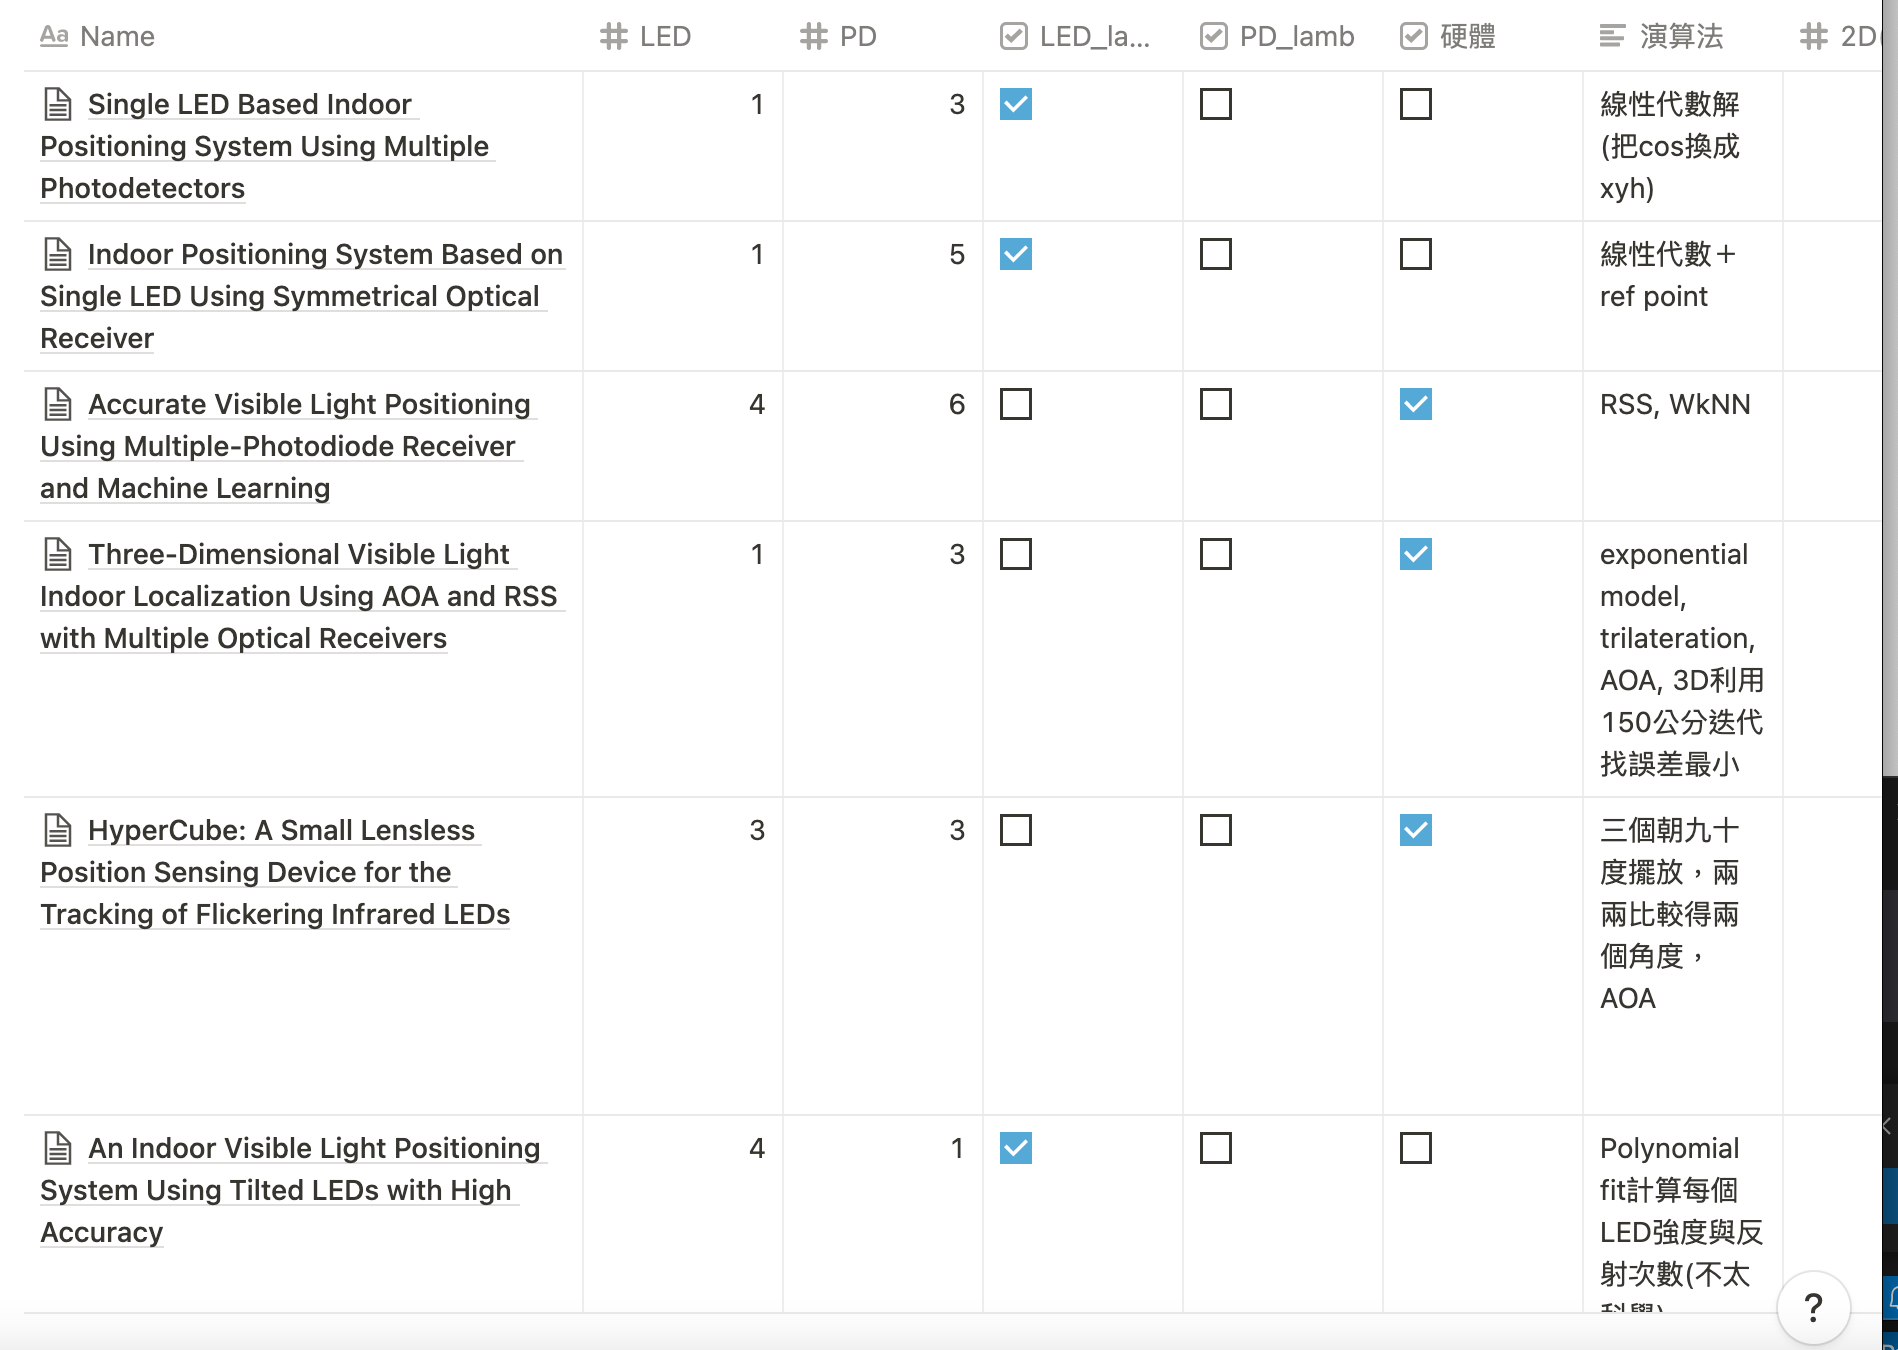
\includegraphics[width=10cm]{00temppic/temp.png}
            % \caption{多重路徑傳輸\cite{pic:multipath}}
            % \label{pic:multipath}
        \end{figure}



\section{結論}

雖然此種做法已被討論且有潛力,但缺少能夠達成三維定位又靈活的方法,也缺乏完整考量硬體擺設方法以及朗博次方的研究,此本論文有以下研究成果:

\begin{itemize}
    \item 利用LED與PD進行三維相對位置量測的方法,於第三章詳述。
    \item 為了將第三章所提出之相對位置量測方法,靈活應用於不同情境,提出針對不同使用情境的最佳化方法,藉由調整硬體參數、LED與PD的組態,改善系統表現,於第四章詳述。
    \item 第五章將提出之最佳化方法實作,以不同情境做為模擬案例,為各自設計最佳的量測系統參數與組態,並進行分析與比較。
    \item 第六章針對本論文的研究成果總結,並提出未來改善方向。
\end{itemize}
\chapter{以LED與PD建立三維相對位置之演算法}
\label{chp:3}

如\ref{chp:LEDPD_problem}章所述,現今LED與PD的定位方法雖具有靈活應用的潛力,然而在單點對單點的定位中,仍未有可以進行三維定位,且不限制目標平面與量測平面平行的方法。因此,本章節將提出一定位演算法,利用$L\times P$個LED對PD的電流大小資訊,計算出三維相對定位,且不需限制目標平面與使用者平面平行,並在模型中將LED與PD的朗博次方考慮進去。

\begin{figure}[h!]
    \centering
    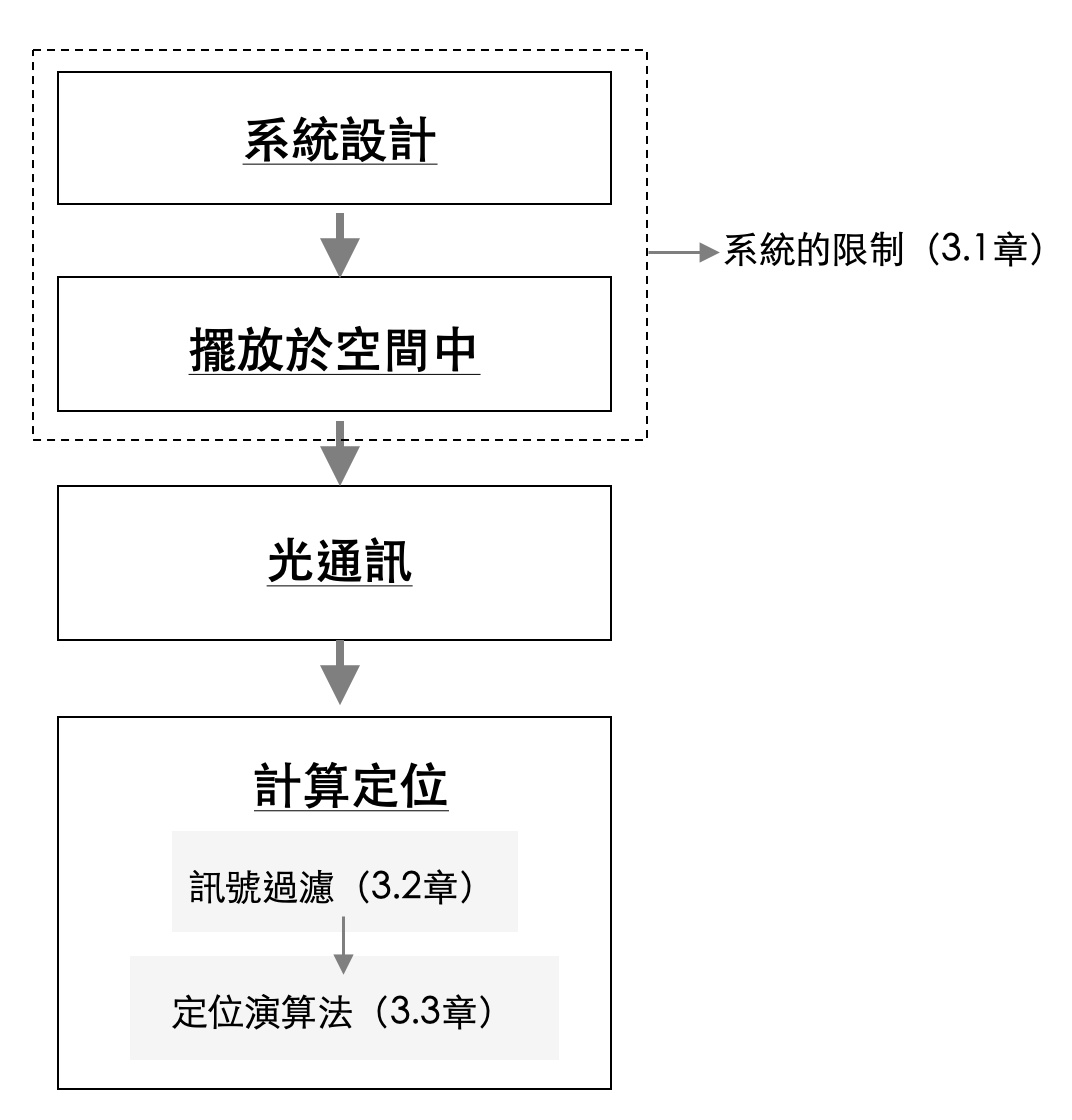
\includegraphics[width=9cm]{ch3pic/chp3_flow.png}
    \caption{第三章章節與定位流程對應}
    \label{pic:chp3_flow}
\end{figure}


本章節的論述順序可以參考圖\ref{pic:chp3_flow},根據LED與PD定位系統流程圖(圖\ref{pic:lp_system_flow})重新整理,著重在計算定位的方法上。首先,\ref{chp:algorithm_constraint}章定義本方法對系統設計的拘束條件,再於\ref{chp:algorithm_filter}章中針對電流資訊進行過濾,於\ref{chp:algorithm}章中解釋如何由過濾過的訊號,計算出三維相對定位,最後於\ref{chp:algorithm_ad_dis}章中整理此演算法的優缺點。








\section{系統的限制}
\label{chp:algorithm_constraint}

根據\ref{chp:LEDPD_problem}章中的論述,我們知道現今文獻上需要透過對系統限制,以將光傳遞模型進行簡化,來求解相對位置。本段落將條列式列出本研究的定位演算法中,使用的系統限制:

    \begin{description}

        \item[1. 硬體選用限制:]系統使用的LED皆為同款式,PD亦然。
        \item[2. PD擺放位置限制:]PD擺放位置相同並於PD座標系原點,$^P\boldsymbol{P}_p=
        \left[\begin{array}{ccc}0&0&0\end{array}\right]^T$
        \item[3. LED擺放位置限制:]LED擺放位置相同並於LED座標系原點,$^L\boldsymbol{P}_l=
        \left[\begin{array}{ccc}0&0&0\end{array}\right]^T$

    \end{description}
   
    \begin{figure}[h!]
        \centering
        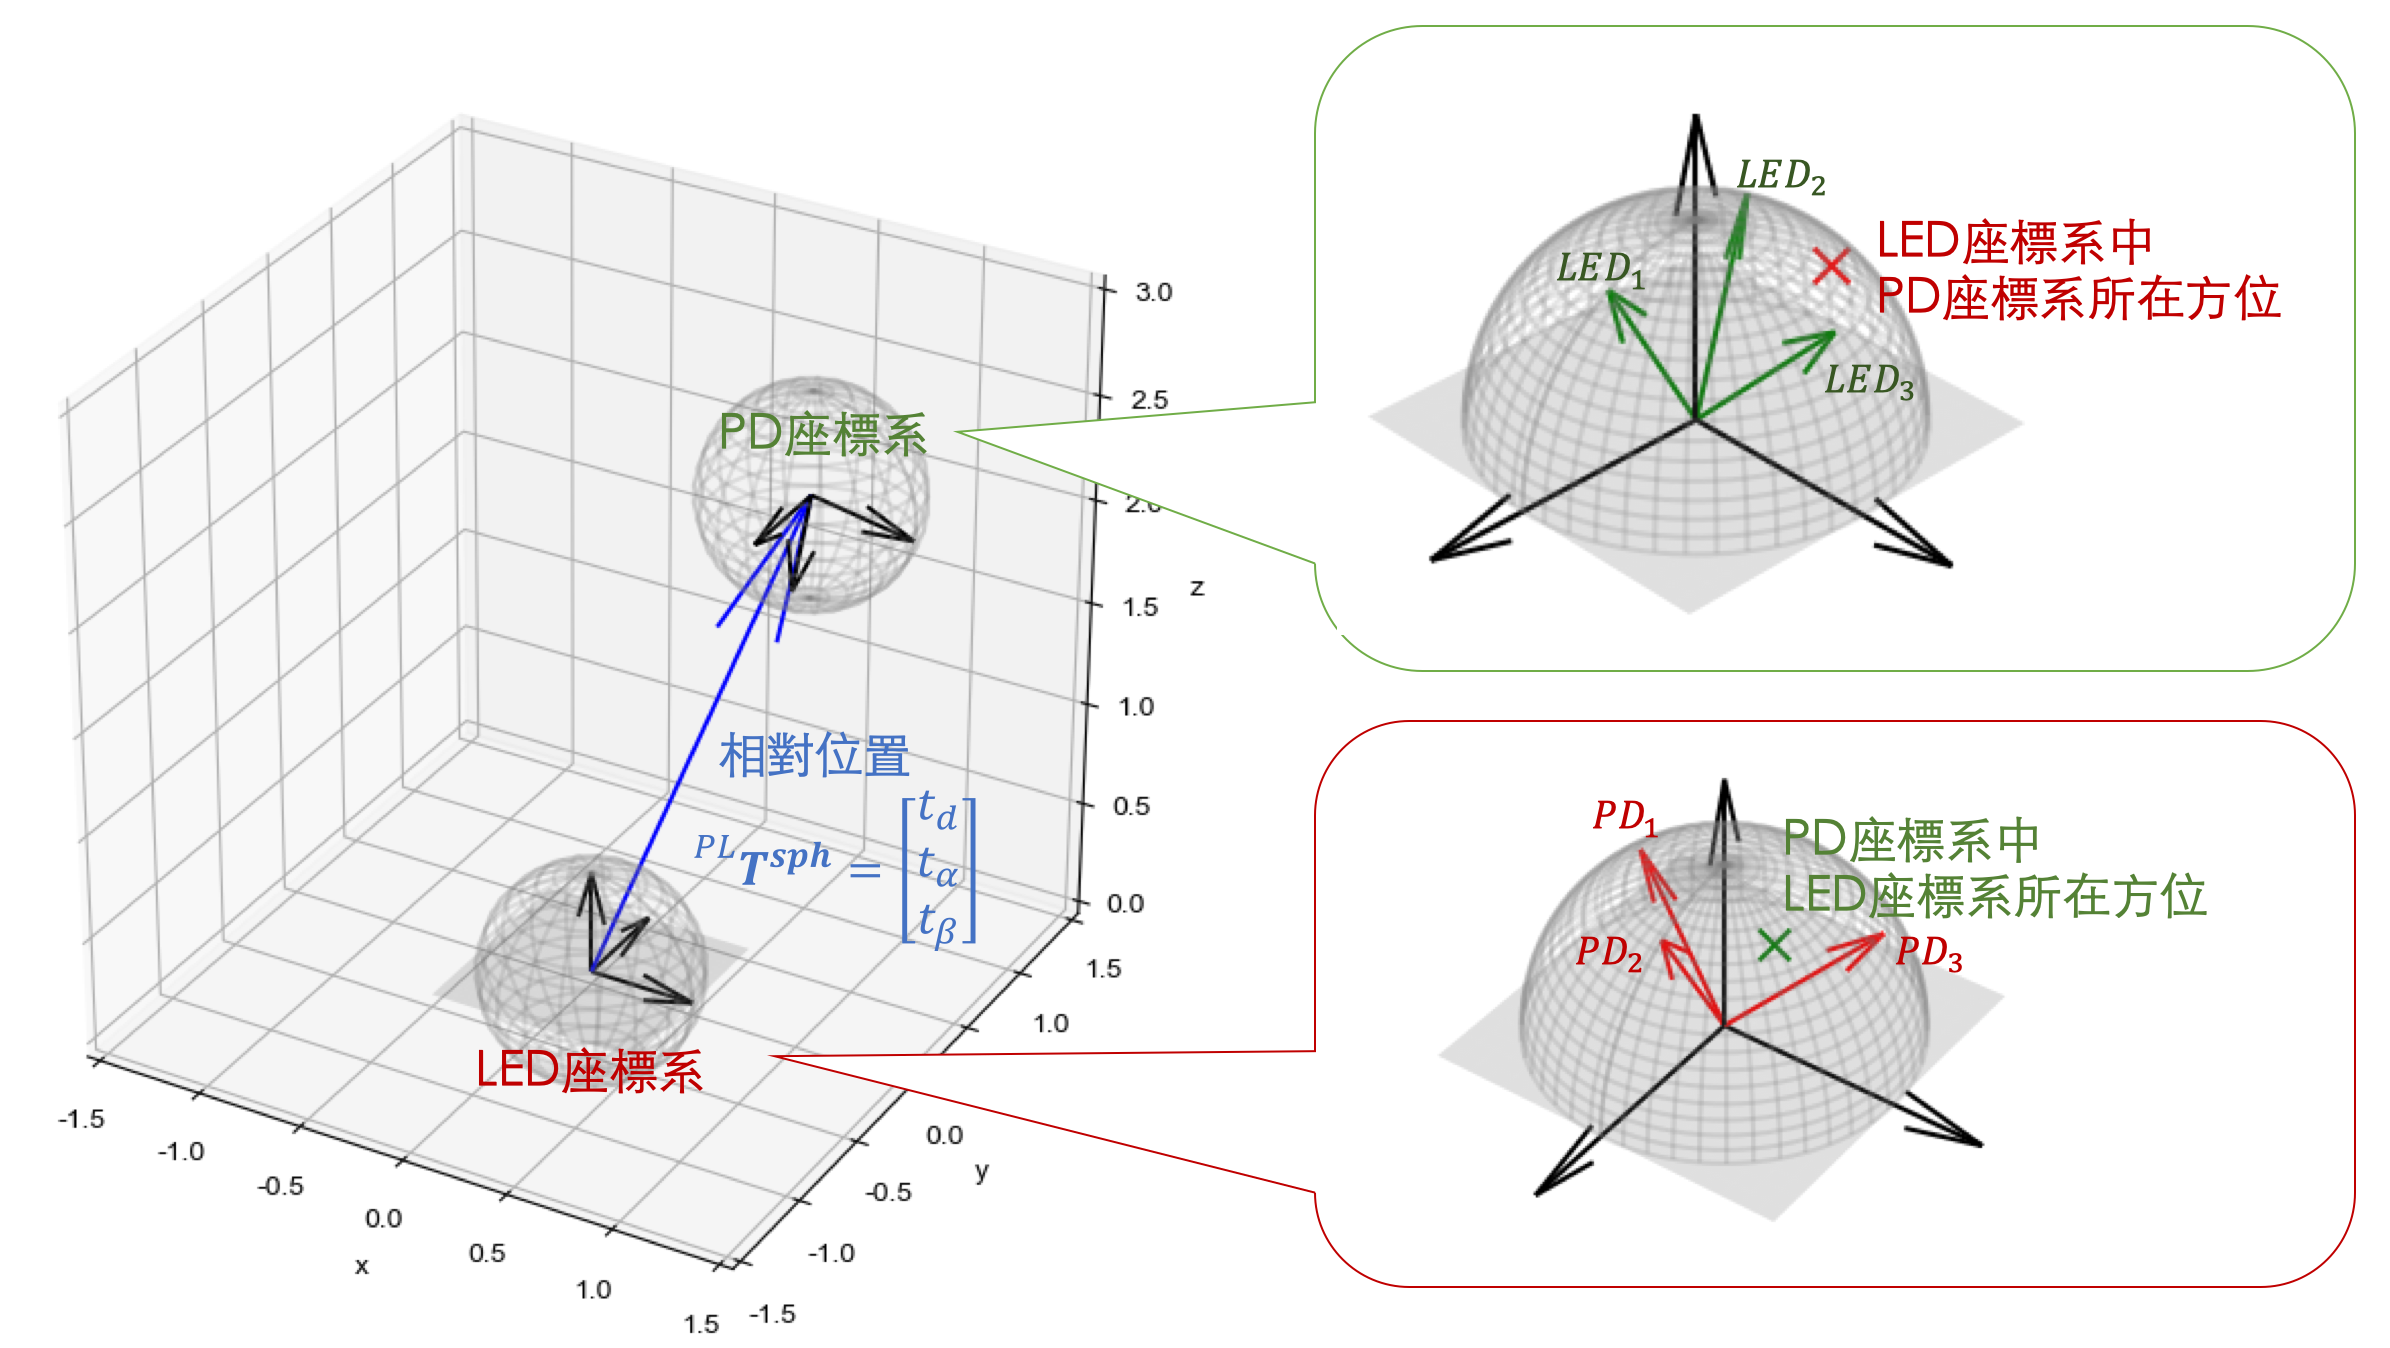
\includegraphics[width=14cm]{ch3pic/algorithm_place.png}
        \caption{PD與LED組態皆限制擺放於原點的系統組態}
        \label{pic:algorithm_coor}
    \end{figure}

    根據以上限制,LED與PD的定位系統可以呈現於圖\ref{pic:algorithm_coor},LED與PD座標系中的硬體皆固定於各自的座標系原點,指向則並無特別限制。在將LED與PD組態設計完成後,座標系放置於空間中兩個點進行定位,其中,各LED到各PD的距離$D_{lp}$皆相同,都是兩座標系之間的距離$t_d$,我們便將光傳遞模型\ref{eqn:model}簡化為\ref{eqn:model_algorithm}。

    \begin{equation}
        \label{eqn:model_algorithm}
        Ie_{lp} = \begin{cases}Re\frac{PtA(Ml+1)}{2\pi}\frac{\cos\phi_{lp}^{Mp}\cos \theta_{lp}^{Ml}}{D^2} , & \text { if } Ie_{lp}<s \\ s, & \text { otherwise }\end{cases}
    \end{equation}

    然而,大多文獻在討輪三維定位時是以卡氏座標系定義相對位置$^{PL}\boldsymbol{T}=\left[\begin{array}{ccc}t_x&t_y&t_z\end{array}\right]^T$,而我們提出的演算法則是以球座標系定義$^{PL}\boldsymbol{T}^{sph}=\left[\begin{array}{ccc}t_d&t_{\alpha}&t_{\beta}\end{array}\right]^T$,因此我們需求出的三個未知數為$t_d,t_\alpha,t_\beta$三項,$t_d$即為兩座標系之間的距離,而$t_{\alpha},t_{\beta}$則為LED座標系所在「方位」。


\section{訊號過濾}
\label{chp:algorithm_filter}

由於PD電流會飽和的特性,已飽和的電流與距離與出入射角無關了,無法用來獲得相對定位,因此我們需將已飽和的電流$Ie_{lp}>s$訊號忽略。除此之外,過小的電流也有可能為雜訊,因此也需設定一閥值$Th$,將小於閥值的電流訊號也忽略,剩餘的訊號則為可運用於計算三維定位的資訊。在訊號過濾後,第$l$個LED中還剩下$Fp_l$個PD電流數值可使用,而第$p$個PD中則剩下$Fl_p$個LED對應的電流數值可使用,參考圖\ref{pic:after_filter}。

\begin{figure}[h!]
    \centering
    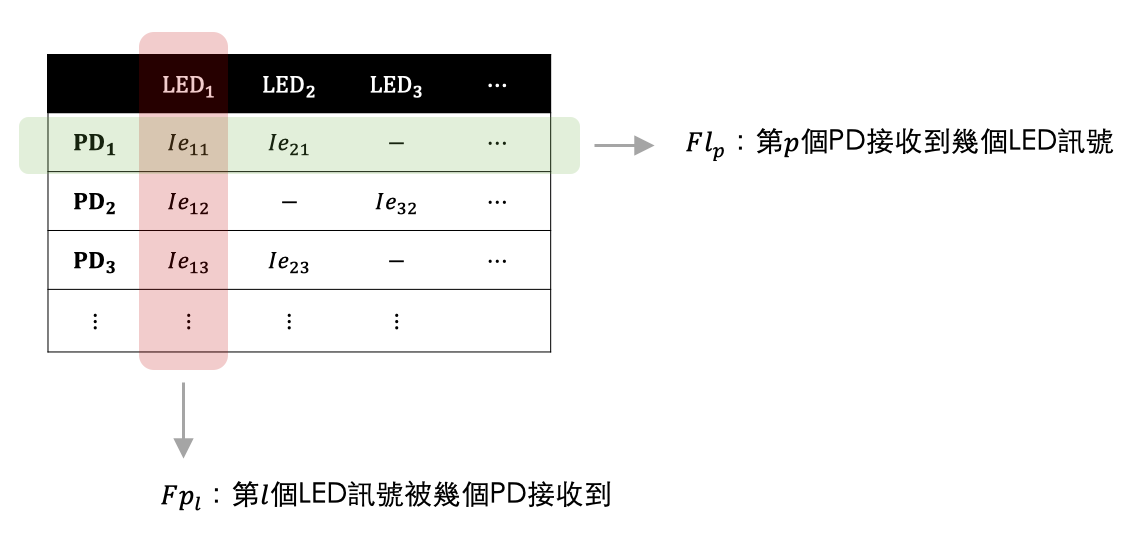
\includegraphics[width=15cm]{ch3pic/after_filter.png}
    \caption{訊號過濾後各LED與各PD所剩的訊號數量示意圖}
    \label{pic:after_filter}
\end{figure}

\section{定位演算法}
\label{chp:algorithm}

\begin{figure}[h!]
    \centering
    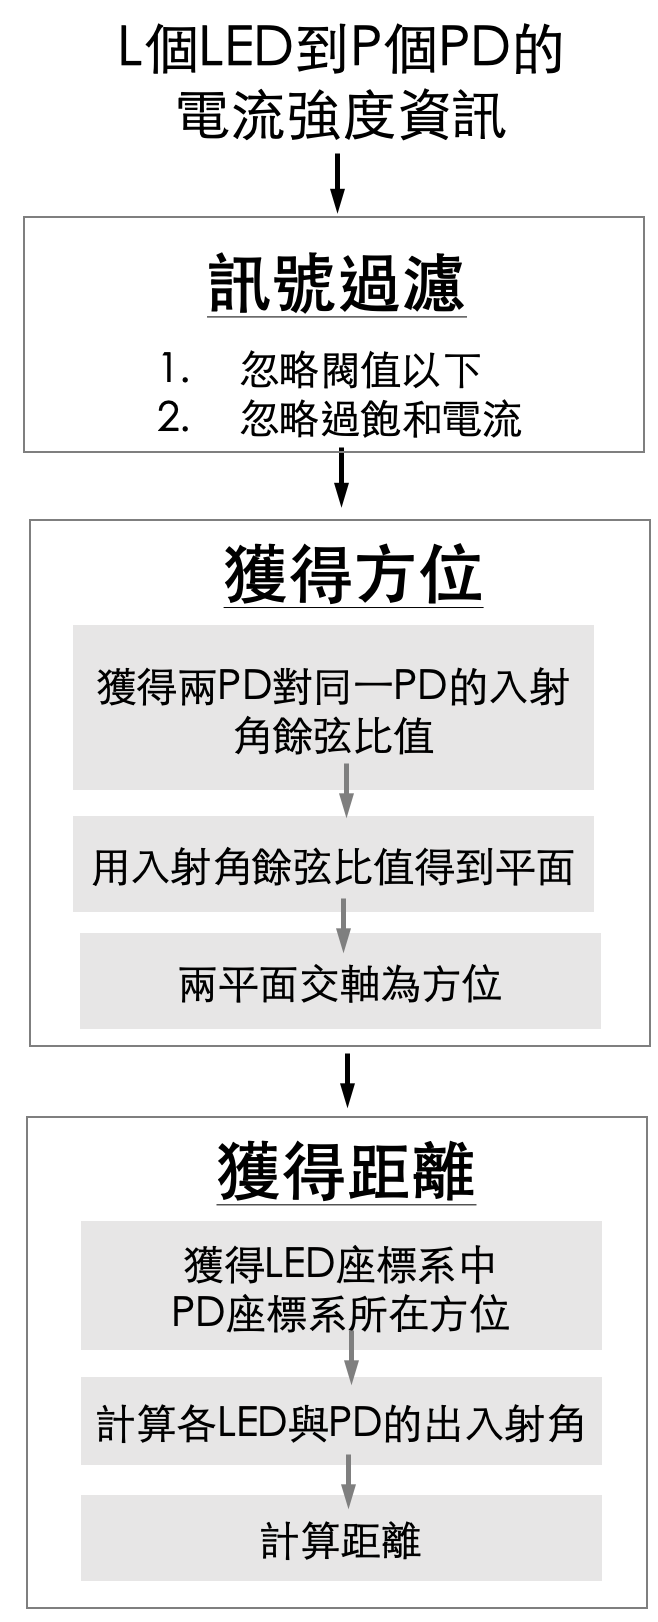
\includegraphics[width=6cm]{ch3pic/algorithm_flow.png}
    \caption{本研究所提出的定位演算法流程}
    \label{pic:algorithm_flow}
\end{figure}

本章結提出的定位演算法,為LED與PD系統流程圖\ref{pic:chp3_flow}中的定位演算法步驟,定位演算法的步驟則呈現於圖\ref{pic:algorithm_flow},依序從\ref{chp:solve_phi}章解出PD座標系中,LED座標系所在方位;\ref{chp:solve_D}綜合LED與PD方位資訊,解出距離。

為了方便表示,將方位以符號表示$^{PL}\boldsymbol{Tv}^{sph} = \left[\begin{array}{ccc}1&t_{\alpha}&t_{\beta}\end{array}\right]^T$,方位為單位向量,可用單位圓表示方位的可行解範圍。





    \subsection{求解方位}
    \label{chp:solve_phi}

    首先,過濾後的訊號即不需考慮過飽和的狀況,因此式\ref{eqn:model_algorithm}可改寫為式\ref{eqn:model_algorithm_filter}。

    \begin{equation}
        \label{eqn:model_algorithm_filter}
        \begin{aligned}
            Ie_{lp}(D_{lp},\theta_{lp},\phi_{lp}) &= Re\frac{PtA(Ml+1)}{2\pi}\frac{{\cos\phi}^{Mp}{\cos\theta}^{Ml}}{D^2}\\
            & = Re\frac{PtA(Ml+1)}{2\pi}\frac{{(^{P}\boldsymbol{V}_p\cdot\boldsymbol{D})}^{Mp}{(-^{PL}\boldsymbol{V}_l\cdot\boldsymbol{D})}^{Ml}}{D^4}
        \end{aligned}
    \end{equation}

    解方位的流程詳細如圖\ref{pic:orient_flow},於\ref{chp:cosine_ratio}章到\ref{chp:orient_average}章詳細介紹取得方位$^{PL}\boldsymbol{Tv}^{sph} = \left[\begin{array}{ccc}1&t_{\alpha}&t_{\beta}\end{array}\right]^T$的過程。

    \begin{figure}[h!]
        \centering
        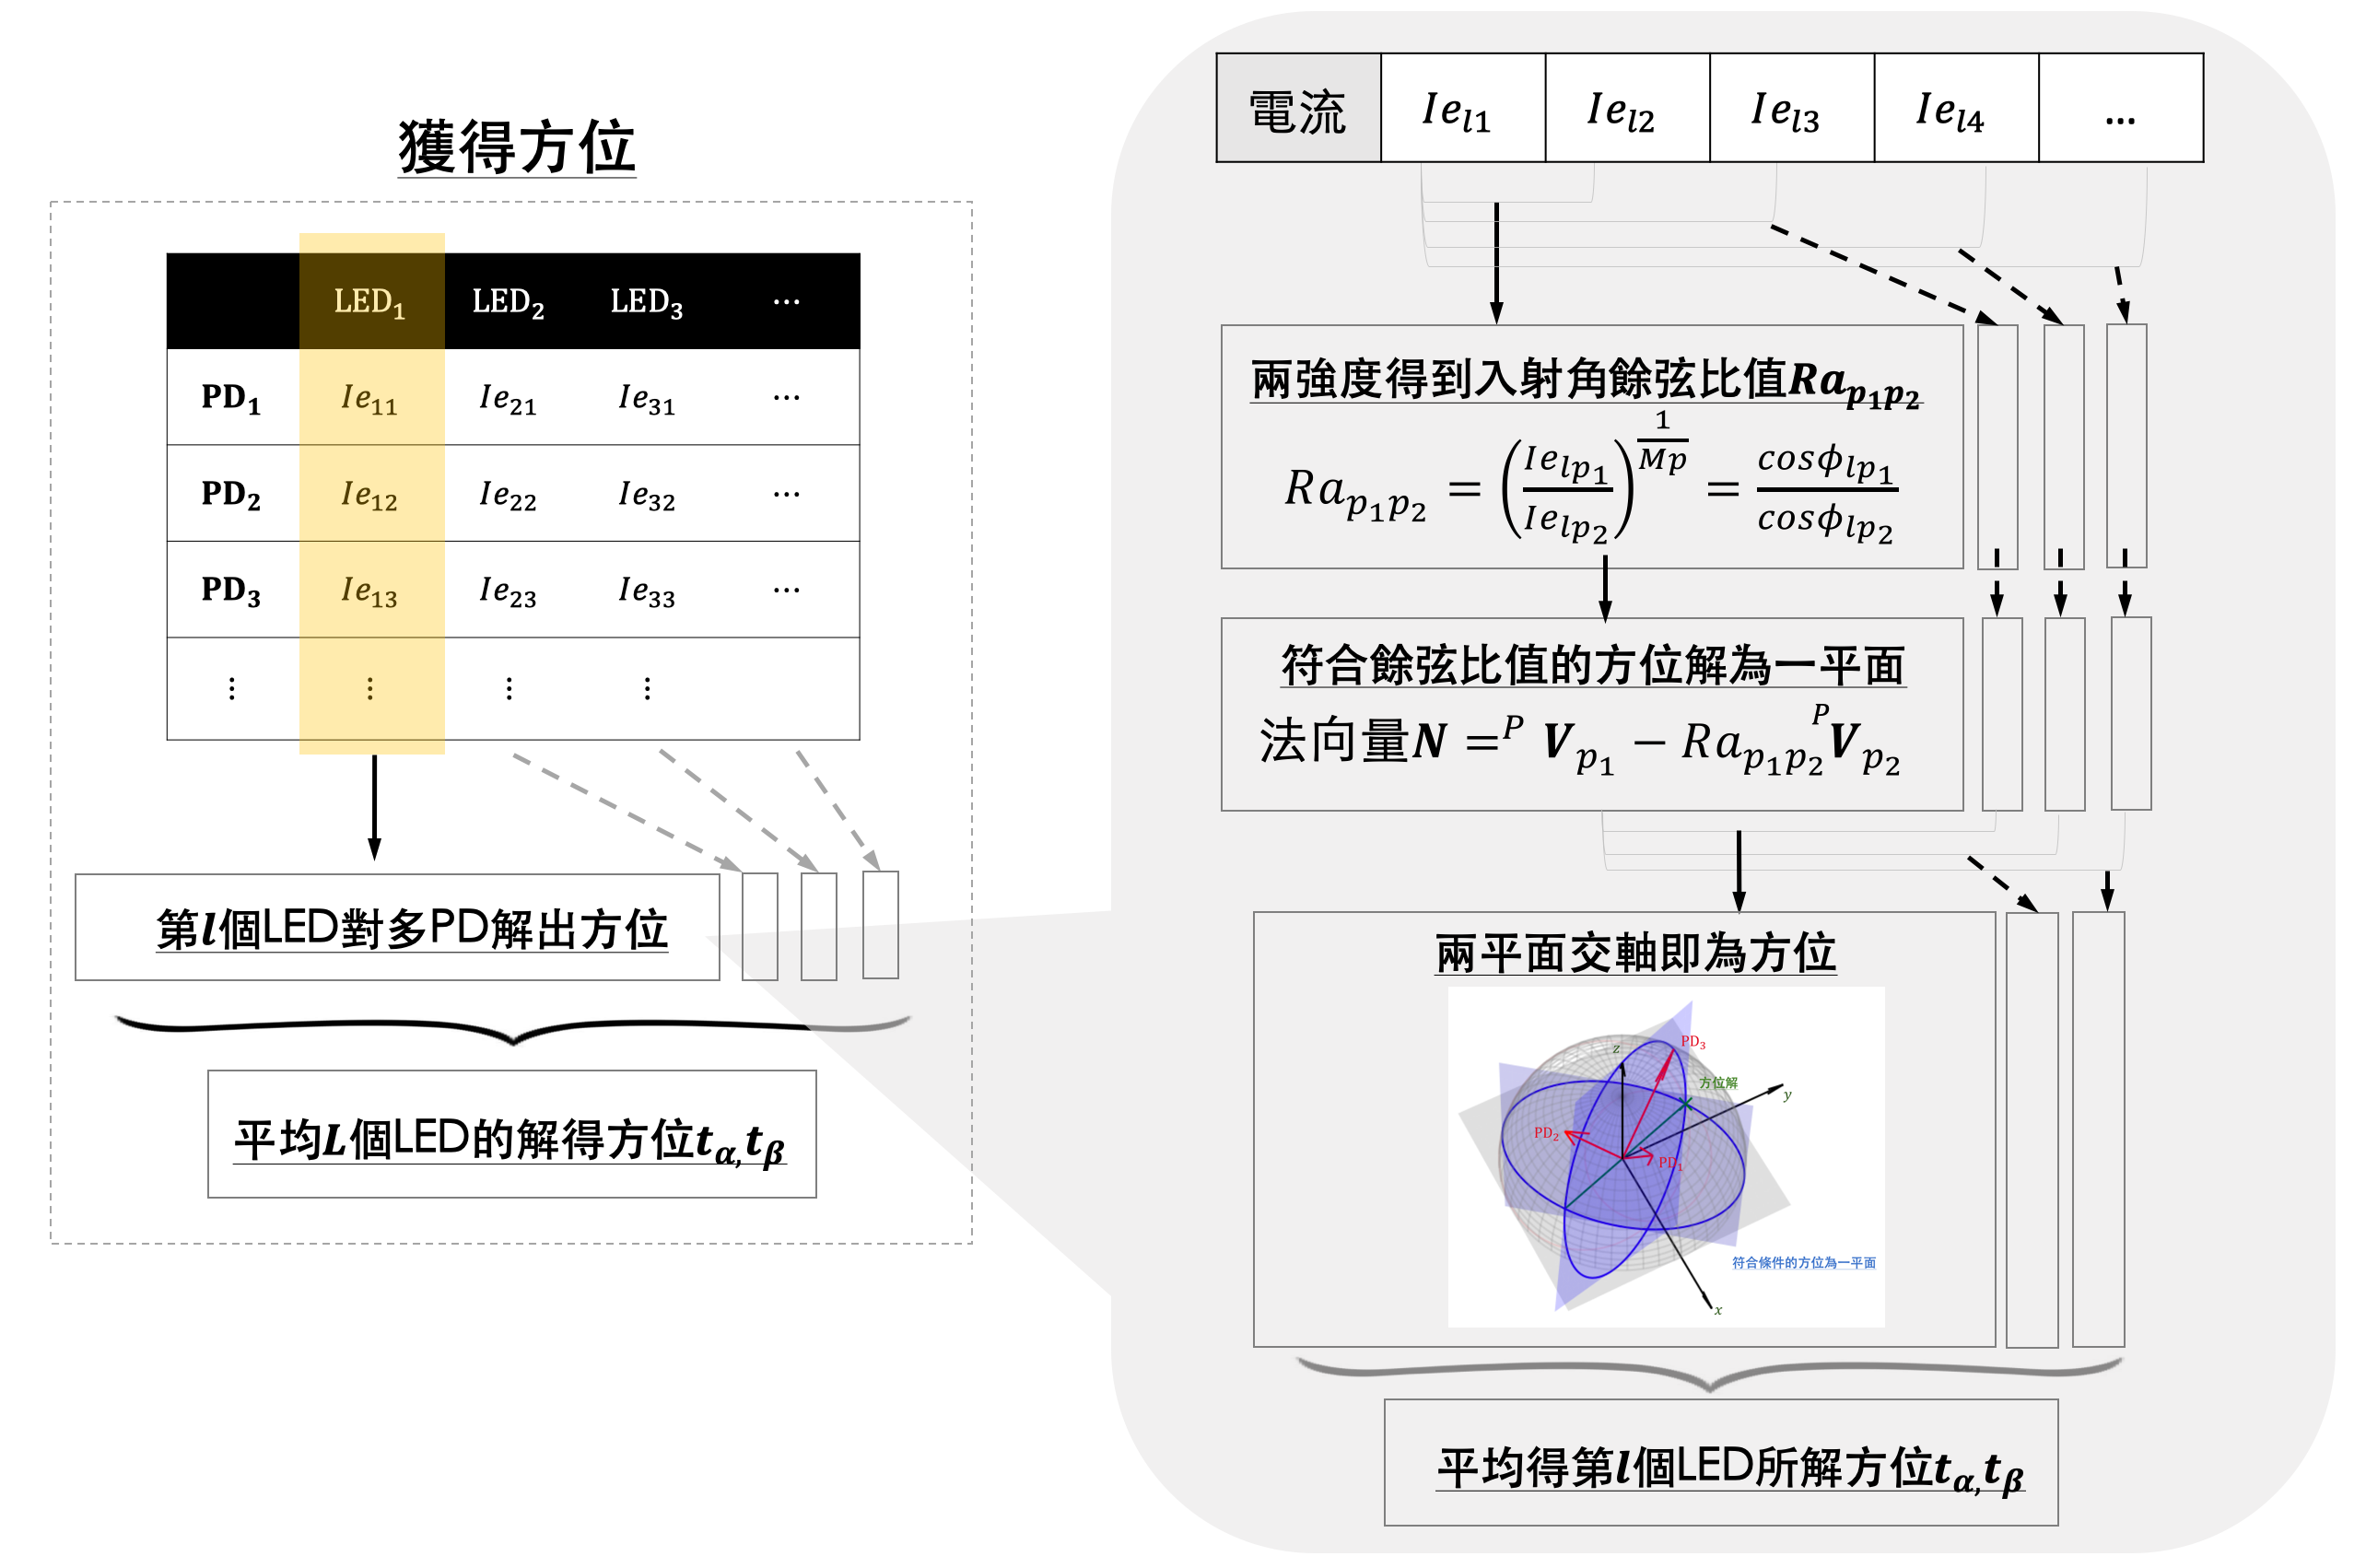
\includegraphics[width=14cm]{ch3pic/orient_flow.png}
        \caption{本研究定位演算法中解方位的流程}
        \label{pic:orient_flow}
    \end{figure}

    \subsubsection{獲得兩PD對同一LED的入射角餘弦比值}
    \label{chp:cosine_ratio}

        \begin{figure}[h!]
            \centering
            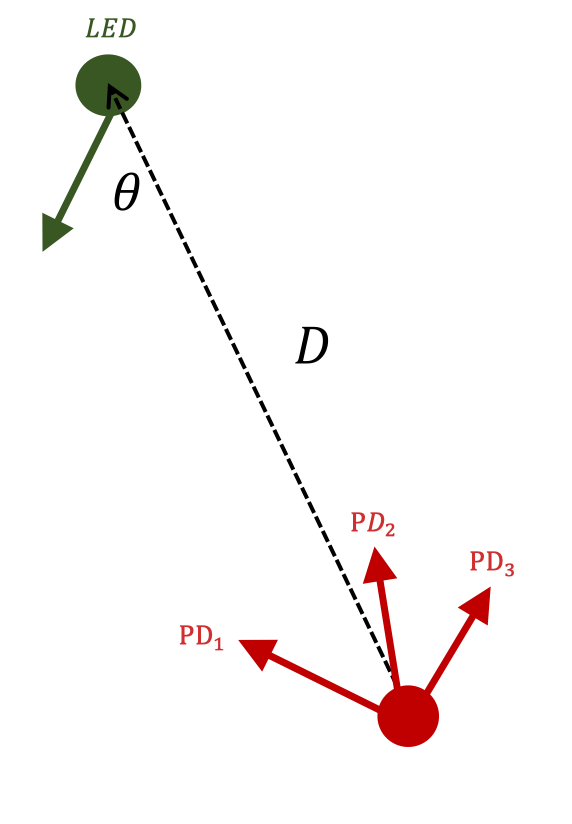
\includegraphics[width=5cm]{ch3pic/1led_mulpd.png}
            \caption{同一LED與多個PD之間的幾何關係}
            \label{pic:1led_mulpd}
        \end{figure}

        當我們僅考慮第$l$個LED的資訊時,如圖\ref{pic:1led_mulpd}所示,各PD與該LED之間的LED出射角$\theta_{lp}$以及距離$D_{lp}$都一樣;因此,式\ref{eqn:model_algorithm_filter}中的三個變數只剩下PD入射角$\phi_{lp}$,而我們於式\ref{eqn:cosine_ratio}中,將不同PD對同樣第$l$個LED的強度訊號相除,可得到入射角餘弦比值的朗博次方。藉由將其開朗博次方根,我們得到編號$p_1$與$p_2$的PD,對第$l$個LED入射角餘弦比值$Ra_{p_1p_2}$。
    
        \begin{equation}
            \label{eqn:cosine_ratio}
            \begin{aligned}
                \frac{Ie_{lp_1}}{Ie_{lp_2}}={(\frac{\cos\phi_{lp_1}} {\cos\phi_{lp_2}})}^{Mp}\\
                Ra_{p_1p_2} = {( \frac{Ie_{lp_1}}{Ie_{lp_2}})} ^{\frac{1}{Mp}} = \frac{\cos\phi_{lp_1}}{\cos\phi_{lp_2}}
            \end{aligned}
        \end{equation}

        兩個PD比較即可得到一個入射角比值,而為了更有系統性的進行兩兩比較,我們選擇一參考PD,其餘PD訊號都與參考PD做比較,即可有效率的完成動作。其中,對第$l$個LED來說,過濾過後的訊號有$Fp_l$個,我們選擇第$r_c$個PD當作參考值,將其作為分母,其他PD電流值與其相比,總共得到$Fp_l-1$個比值$Ra_{pr_c}$

    \subsubsection{滿足入射角餘弦比值的方位解位於一通過原點之平面}
    \label{chp:solve_surface}
        
        於式\ref{eqn:cosine_ratio}中得到兩入射角餘弦比值,而我們需要從餘弦比值中得到方位關係,雖然兩角度的餘弦比值並沒有單一解,但是滿足入射角餘弦比值$Ra_{pr_c}$的方位解$^{PL}\boldsymbol{Tv}$,僅有可能位於一通過原點之平面,以下進行推導。
        
        首先,將式\ref{eqn:cosine_ratio}中的PD入射角$\phi_{lp}$,改寫為PD指向$^P\boldsymbol{V}_p$與入射方位$^{PL}\boldsymbol{Tv}$的內積,如式\ref{eqn:phi2dot}。
     

        \begin{equation}
            \label{eqn:phi2dot}
            \begin{aligned}
                \because \cos\phi_{lp} = ^{PL}\boldsymbol{Tv}\cdot^P\boldsymbol{V}_p\\
                \therefore Ra_{p_1r_c}
                =\frac{^{PL}\boldsymbol{Tv}\cdot^P\boldsymbol{V}_{p_1}}{^{PL}\boldsymbol{Tv}\cdot^P\boldsymbol{V}_{r_c}}
            \end{aligned}
        \end{equation}
        % \begin{equation}

        而式\ref{eqn:phi2dot}中的向量都以卡氏座標系展開,經過移項整理呈現於式\ref{eqn:surface}。

            \begin{gather}
                 \label{eqn:surface}
                 ^{PL}\boldsymbol{Tv} \cdot(Ra_{p_1r_c} ^P\boldsymbol{V}_{r_c}-
                 ^P\boldsymbol{V}_{p_1})=0
            \end{gather}
        % \end{equation}

        式\ref{eqn:surface}中的方位$^{PL}\boldsymbol{Tv}$,於空間中為一通過原點的平面,參考圖\ref{pic:solve_surface},透過兩個PD強度比較,我們可以得到一個方位解的可能平面。
       

       \begin{figure}[h!]
        \centering
        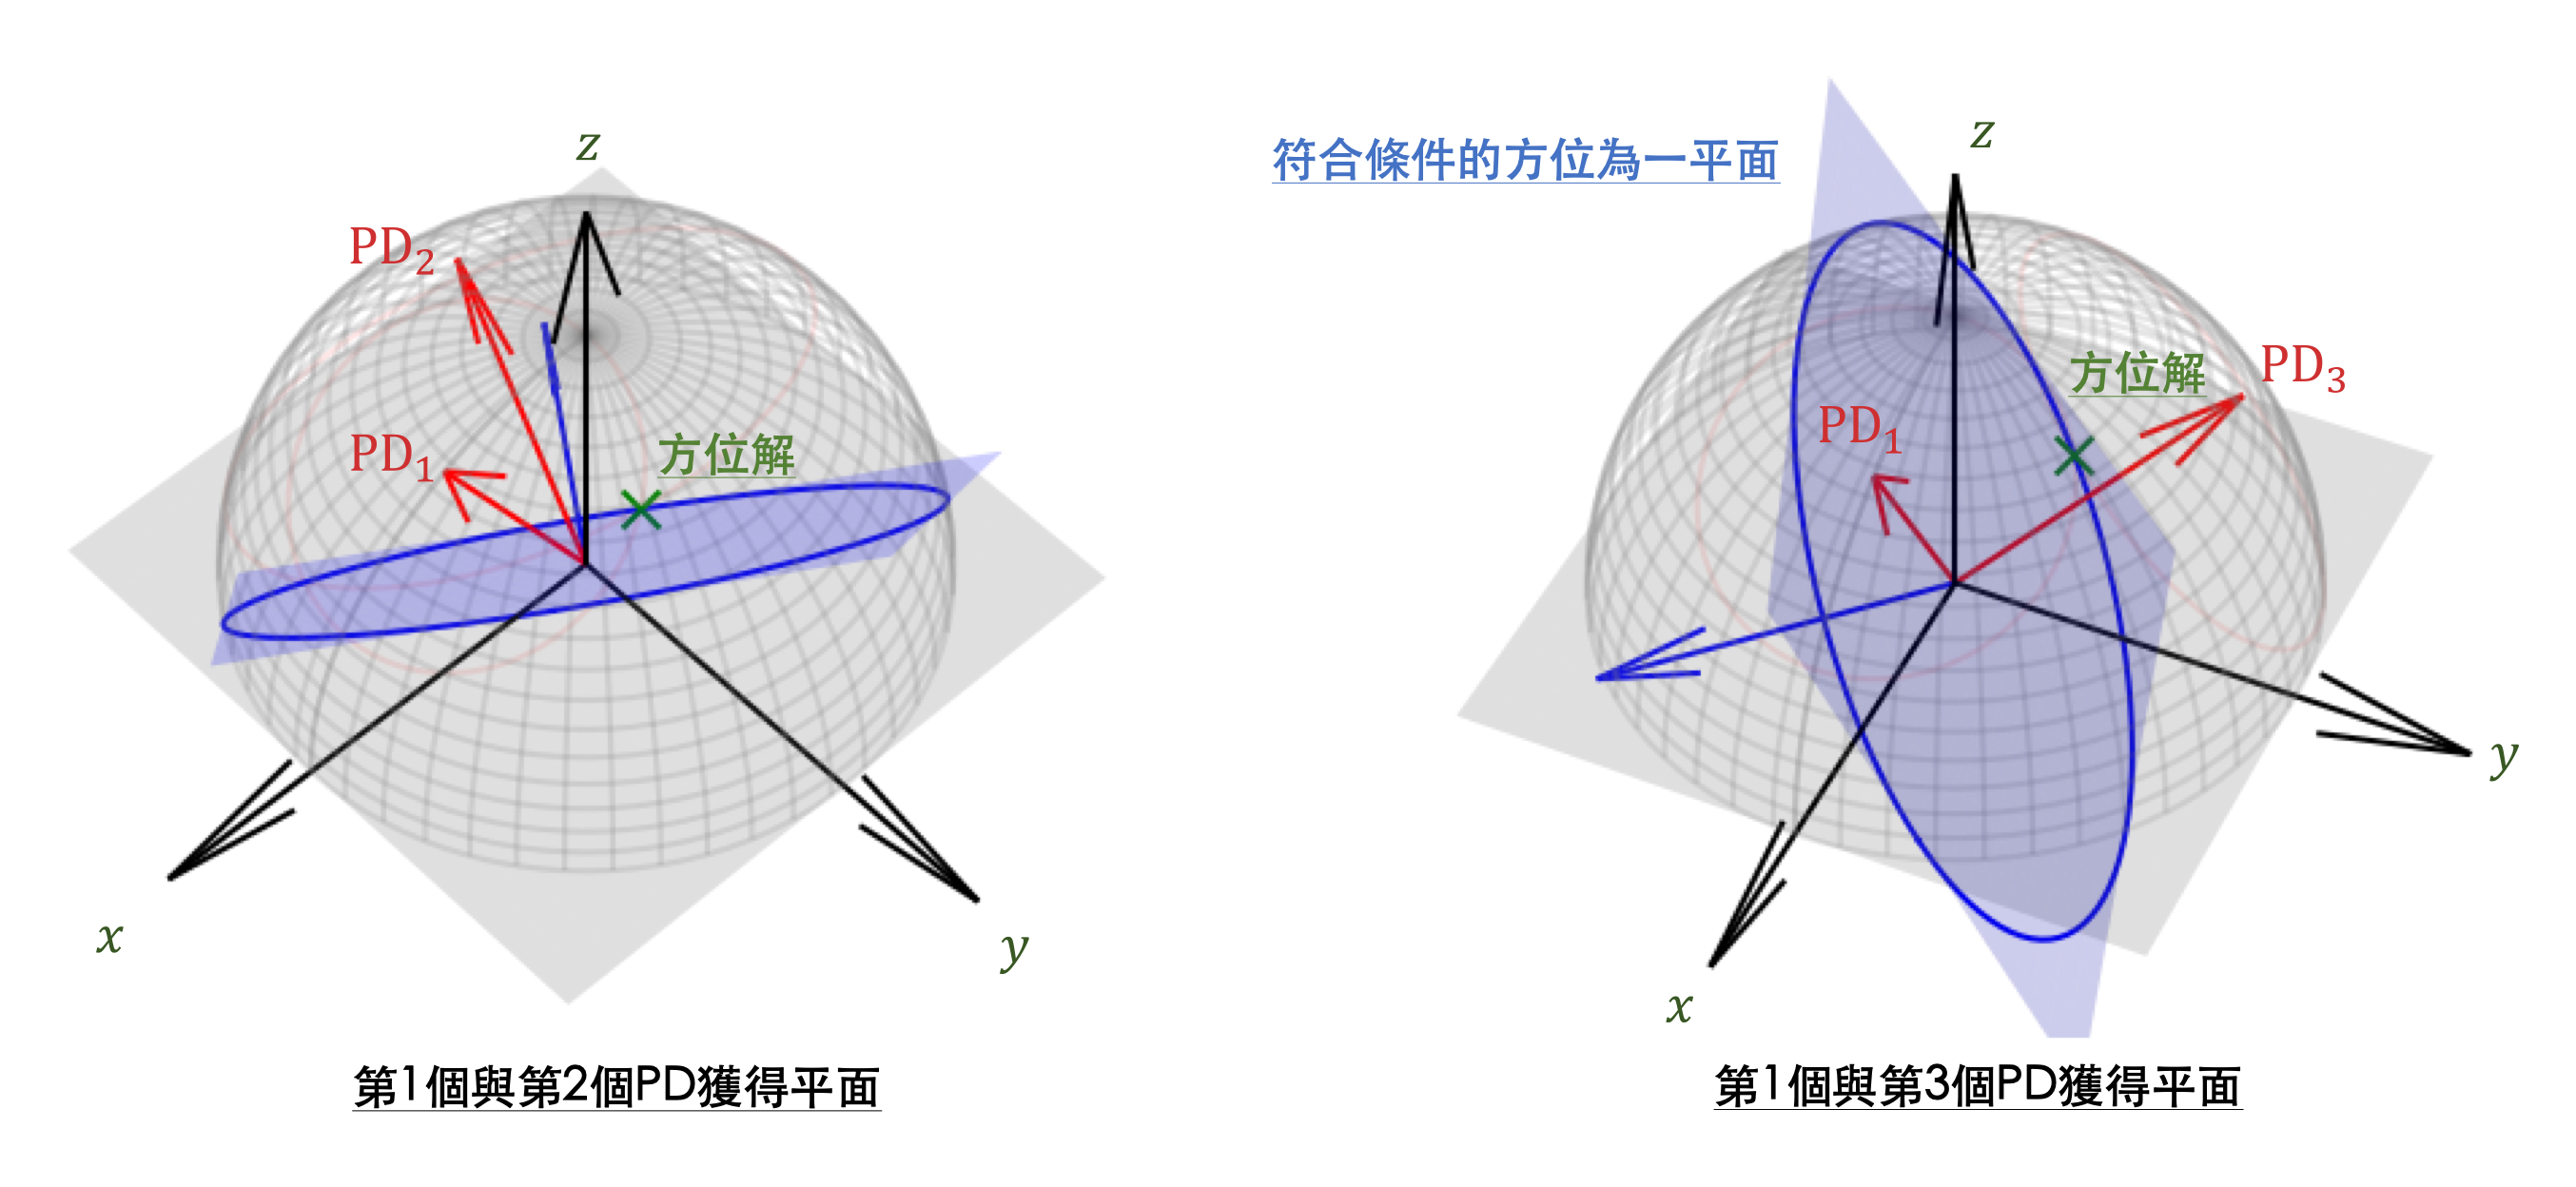
\includegraphics[width=14cm]{ch3pic/solve_surface.png}
        \caption{滿足入射角餘弦比值$Ra$的方位為通過原點之平面}
        \label{pic:solve_surface}
        \end{figure}

         
        我們將平面法向量以$\boldsymbol{N}_{p_1r_c}$表示於式\ref{eqn:surface_normal}中,小標$p_1,r_c$代表該平面是由第$p_1$個PD與第$r_c$個PD的入射角餘弦比值計算而得,其中$r_c$為作為參考值的PD編號。
        
        \begin{gather}
            \label{eqn:surface_normal}
            \boldsymbol{N}_{p_1r_c}  = {Ra_{p_1r_c}}{} ^P\boldsymbol{V}_{r_c}-
            ^P\boldsymbol{V}_{p_1}
       \end{gather}
        
        而於\ref{chp:cosine_ratio}章中,我們知道對第$l$個LED可以得到$Fp_l-1$個入射角餘弦比值$Ra_{pr_c}$,在本段我們將這些比值換算成$Fp_l-1$個平面。值得注意的是,因為所解方位只有兩個自由度,方位唯一單位長度的向量,因此符合藉兩PD入射角餘弦比值的方位解,為通過原點平面上的單位圓。


    \subsubsection{兩平面交軸為方位}
    \label{chp:solve_axis}

        由\ref{chp:solve_surface}章中,我們知道滿足兩PD入射角餘弦比值$Ra_{pr_c}$的方位為一通過原點之平面上的單位圓。為了得到入射方位,我們將平面兩兩取交軸,交軸則為可能方位。兩兩取交軸與\ref{chp:solve_surface}章相同,本小節同樣取一平面作為參考,該平面為第$r_c$與$r_s$個PD入射角比值$Ra_{r_sr_c}$所得到的平面,參考平面的平面法向量為$\boldsymbol{N}_{r_sr_c}$。
        
        \begin{figure}[h!]
            \centering
            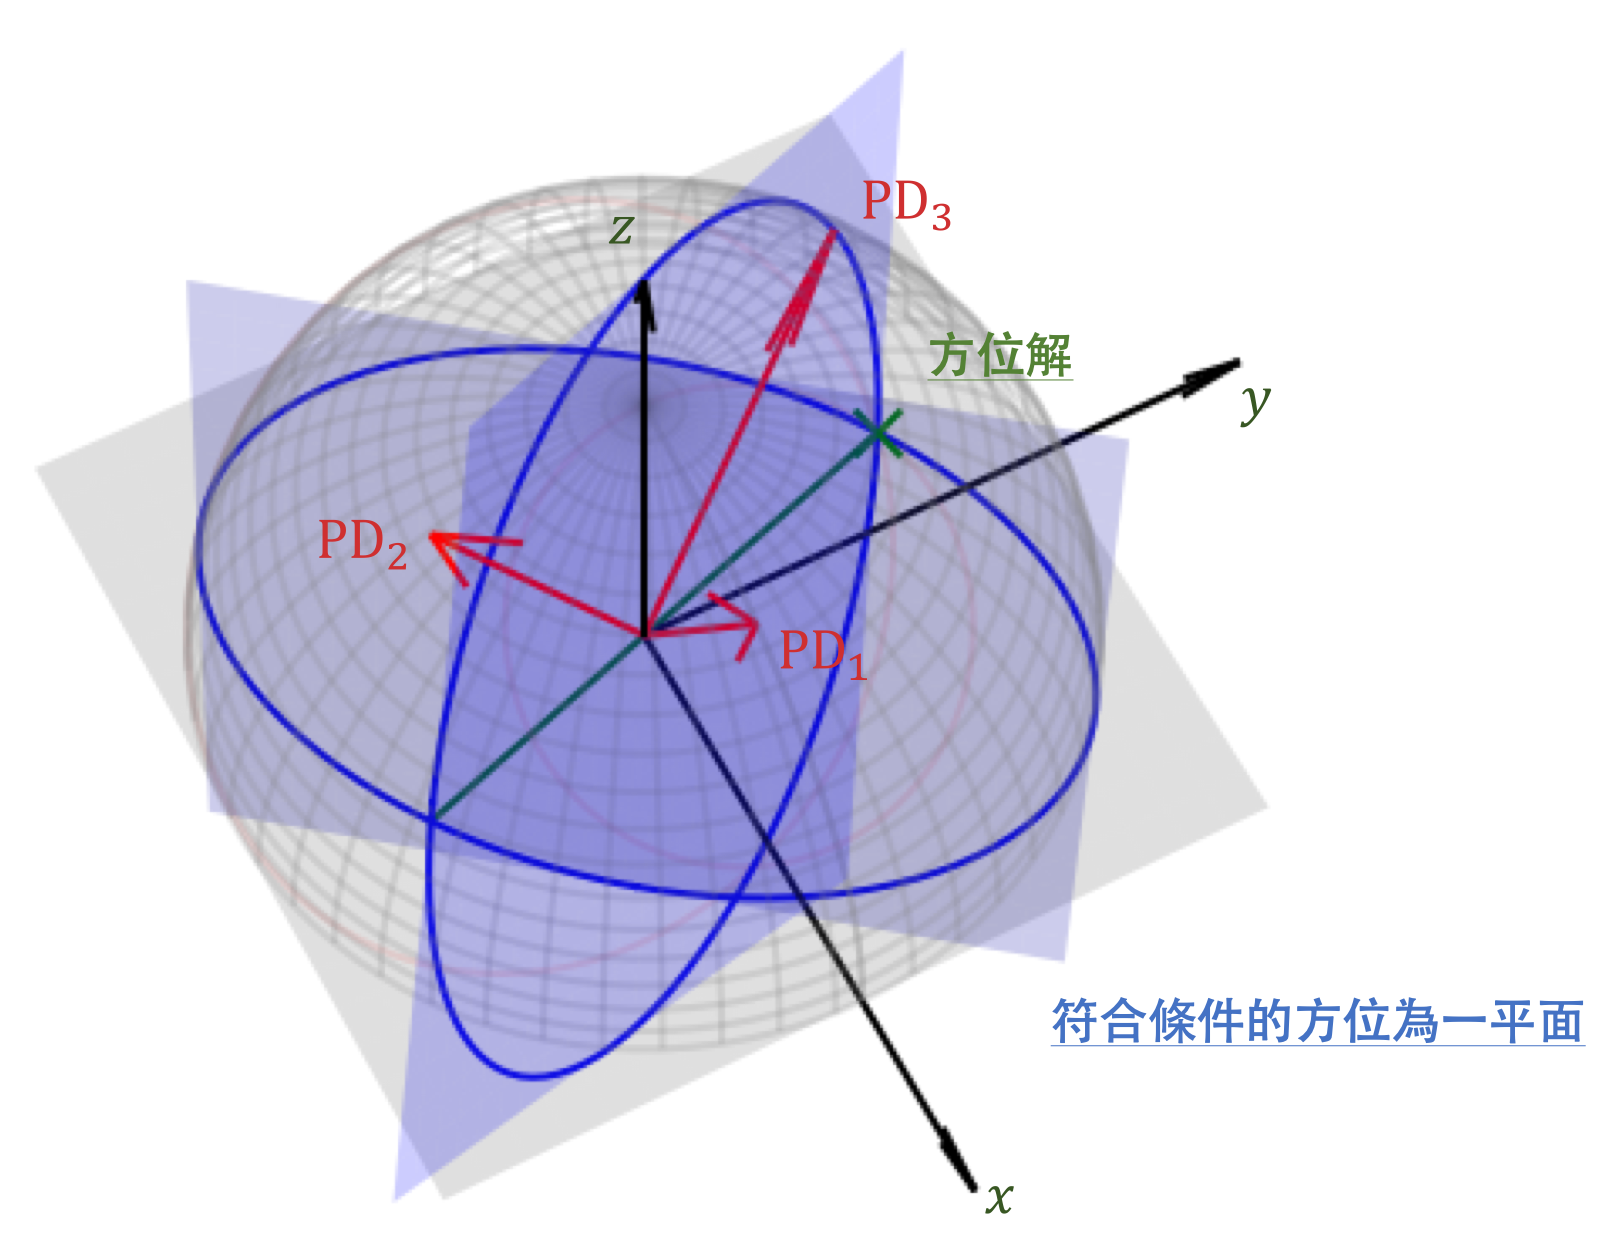
\includegraphics[width=9cm]{ch3pic/solve_axis.png}
            \caption{兩平面交於一軸}
            \label{pic:solve_axis}
        \end{figure}

        其中,兩平面交軸有正負兩個方向,我們可以透過PD可視範圍最大為$90^o$的特性,判斷出方位解為交軸的正方向還是負方向,呈現於式\ref{eqn:solve_axis}。
   
        \begin{gather}
            \label{eqn:solve_axis}
             \hat{{^{PL}\boldsymbol{Tv}}_{p{r_sr_c}}} = 
             \begin{cases}
                (\boldsymbol{N}_{pr_c}\times \boldsymbol{N}_{r_sr_c})&,(\boldsymbol{N}_{pr_c}\times \boldsymbol{N}_{r_sr_c})>0\\
                -(\boldsymbol{N}_{pr_c}\times \boldsymbol{N}_{r_sr_c})&,\text{else}
             \end{cases}
        \end{gather}

        在此步驟,我們利用\ref{chp:cosine_ratio}章中產生的$Fp_l-1$個平面,選擇其中一個作為參考平面,將他以外的$Fp_l-2$個平面與其參考平面外積,得到共$Fp_l-2$個計算出的方位$\hat{{^{PL}\boldsymbol{Tv}}_{p{r_sr_c}}}$。


    \subsubsection{平均方位}
    \label{chp:orient_average}

        第$l$個LED與PD的電流資訊,可以解出$Fp_l-2$個方位,因此\textbf{該LED過濾後的訊號最少需被3個PD感測到,才得以解出方位。}而我們將$Fp_l-2$個方位平均,得到第$l$個LED利用$Fp_l$個資訊求出的方位$\hat{{^{PL}\boldsymbol{Tv}}_{l}}$。
        \begin{equation}
            \label{eqn:average_orient_led}
            \hat{{^{PL}\boldsymbol{Tv}}_{l}} = \frac{\sum^{Fp_l-2}_{p=1}\hat{{^{PL}\boldsymbol{Tv}}_{p{r_sr_c}}}}{Fp_l-2}
        \end{equation}

        而一共有$l$個LED,我們再將$l$個LED獲得的方位$\hat{{^{PL}\boldsymbol{Tv}}_{l}}$平均,解出方位$\hat{{^{PL}\boldsymbol{Tv}}}$。

        \begin{equation}
            \label{eqn:average_orient}
            \hat{{^{PL}\boldsymbol{Tv}}} = \frac{\sum^{L}_{l=1}\hat{{^{PL}\boldsymbol{Tv}}_{l}}}{L}
        \end{equation}
        
        
    \subsubsection{小結}
    \label{chp:orient_conclu}

    計算方位的方法,是透過PD兩兩比較得到方位的可能平面解,再透過平面兩兩外積求交軸即為方位。然而由於$L$個LED與$P$個PD交互之下,兩兩比較便會變得很複雜,可以參考圖\ref{pic:algorithm_flow}中的流程較為清楚。在這之中,最少需要一個LED與三個訊號沒被過濾掉的PD訊號,才能夠解出方位。

        

         

    


    \subsection{求解距離}
    \label{chp:solve_D}

    在\ref{chp:solve_phi}章中解出方位後,對於光傳遞模型(式\ref{chp:model_mul})中的變數,我們目前僅能夠得到入射角$\phi_{lp}$的資訊,仍缺少出射角資訊以求距離。因此,求解距離的步驟可參考圖\ref{pic:algorithm_flow},需要先解出PD座標系於LED座標系上的方位,再利用方位資訊解出出入射角,進而利用光傳遞模型解出距離,以下分小節介紹。

        \subsubsection{解LED座標系中PD座標系所在方位}
        \label{chp:solve_theta}

        我們可以利用\ref{chp:solve_phi}章中一樣的方法,改應用在LED座標系中,解出PD座標系於LED座標系上的方位$\hat{{^{LP}\boldsymbol{Tv}}}$。方法與\ref{chp:solve_phi}章完全相同,以下僅簡單介紹:

        針對第$p$個PD的資訊,在訊號過濾後,總共接收到$Fl_p$個LED訊號。而由於硬體擺放位置皆限制於座標系原點,因此參考圖\ref{pic:mulled_1pd},式\ref{eqn:model_algorithm_filter}中的三個變數僅剩下LED出射角$\theta_{lp}$,即可透過兩兩比較,得到$Fl_p-1$個出射角餘弦比值,而滿足出射角餘弦比值的方位為通過原點的平面。
        
        \begin{figure}[h!]
            \centering
            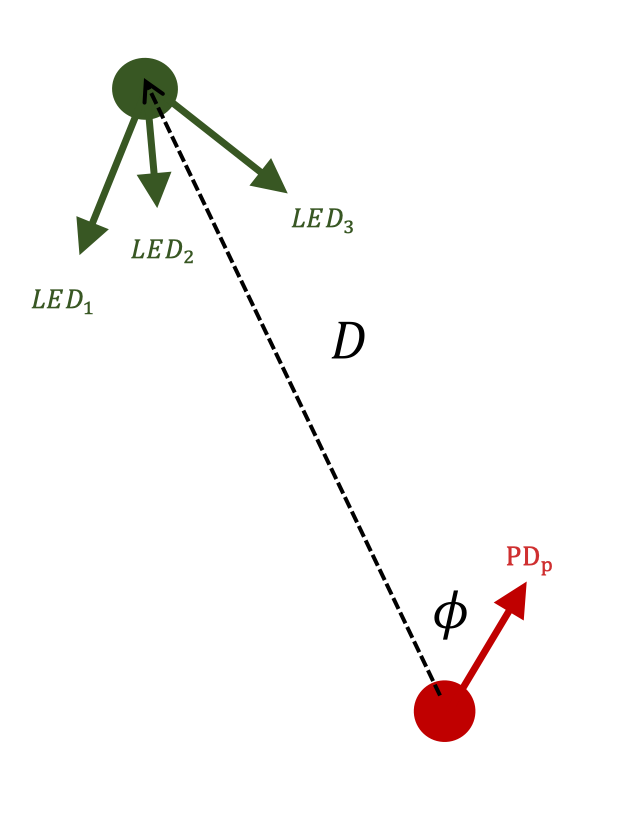
\includegraphics[width=6cm]{ch3pic/mulled_1pd.png}
            \caption{多LED對同一PD之間的幾何關係}
            \label{pic:mulled_1pd}
        \end{figure}

        再來,同樣取一平面作為參考,將其餘平面與參考平面外積,得到共$Fl_p-2$個方位$\hat{{^{LP}\boldsymbol{Tv}_{lr_sr_c}}}$(參考式\ref{eqn:solve_axis})。最後將第$p$個PD獲得的$Fl_p-2$個方位平均得$\hat{{^{LP}\boldsymbol{Tv}_{p}}}$,再將總共$P$個PD所得方位平均,即可獲得PD座標系於LED座標系上的方位$\hat{{^{LP}\boldsymbol{Tv}}}$,可以參考圖\ref{pic:algorithm_coor}。


        \subsubsection{解出LED與PD的出入射角}
        \label{chp:solve_ang}

        有了\ref{chp:solve_phi}章中求出的PD座標系中LED所在方位$\hat{{^{PL}\boldsymbol{Tv}}}$,我們利用PD硬體指向$^P\boldsymbol{V}_p$與方位的內積獲得各PD的入射角$\hat{\phi_{lp}}$,如式\ref{eqn:solve_inang}。
        
        \begin{equation}
            \label{eqn:solve_inang}
            \hat{\phi_{lp}} = \arccos(\hat{{^{PL}\boldsymbol{Tv}}}\cdot ^P\boldsymbol{V}_p)
        \end{equation}
        
        出射角則是利用\ref{chp:solve_theta}章中求出PD座標系於LED座標系的方位$\hat{{^{LP}\boldsymbol{Tv}}}$,同樣與LED指向內積,得到各LED的出射角$\hat{\theta_{lp}}$,如式\ref{eqn:solve_outang}。

        \begin{equation}
            \label{eqn:solve_outang}
            \hat{\theta_{lp}} = \arccos(\hat{{^{LP}\boldsymbol{Tv}}}\cdot ^L\boldsymbol{V}_l)
        \end{equation}

        \subsubsection{利用光傳遞模型取得距離並平均}
        \label{chp:dis_average}

        光傳遞模型中(式\ref{eqn:model_algorithm_filter}),三個變數中的出入射角$\theta\phi$,已於式\ref{eqn:solve_outang}與式\ref{eqn:solve_inang}中求得,因此可求出唯一未知的變數距離$D$,呈現於下式\ref{eqn:solve_dis}

        \begin{equation}
            \label{eqn:solve_dis}
            \begin{aligned}
            \hat{t_d },_{lp} &= \sqrt[2]{\frac{ReAPt (Ml_{l}+1)}{2\pi}
                \frac{\cos\phi_{lp}^{Mp_{p}}\cos \theta_{lp}^{Ml_{l}} }
                {Ie_{lp}}
            }\\
            & = \sqrt[2]
            {
                \frac{ReAPt (Ml_{l}+1)}{2\pi}
                \frac{
                    (\hat{{^{PL}\boldsymbol{Tv}}}\cdot ^P\boldsymbol{V}_p)^{Mp_{p}}
                    (\hat{{^{LP}\boldsymbol{Tv}}}\cdot ^L\boldsymbol{V}_l)^{Ml_{l}} }
                {Ie_{lp}}
            }
            \end{aligned}
        \end{equation}


        式\ref{eqn:solve_dis}中得到的$L\times P$個距離解,於式\ref{eqn:average_dis}中平均得到解。

        \begin{equation}
            \label{eqn:average_dis}
            \hat{t_d }= \frac{\sum^{L}_{l=1}\sum^{P}_{p=1} \hat{t_d },_{lp} }{L\times P}
        \end{equation}

        \subsubsection{小結}

        如\ref{chp:orient_conclu}章所述,最少需要一個LED與3個PD才能獲得方位$\hat{{^{PL}\boldsymbol{Tv}}}$;而概念相同,PD座標系於LED座標系中的方位$\hat{{^{LP}\boldsymbol{Tv}}}$,則需要至少一個PD與3個LED才能解,進而得到距離資訊。\textbf{綜合兩者,我們需要最少三個LED對三個PD才能同時得到LED與PD於對方座標系中的方位$\hat{{^{PL}\boldsymbol{Tv}}}$,進而解出距離$\hat{t_d}$。}綜合方位與距離,相對位置以卡氏座標系表示如式\ref{eqn:solu}


        \begin{equation}
            \label{eqn:sollu}
            \hat{^{PL}\boldsymbol{T} }= \hat{t_d} \times {^{PL}\boldsymbol{Tv}} 
        \end{equation}

\section{演算法優點與缺點}
\label{chp:algorithm_ad_dis}


介紹完本研究所提出的演算法,這裡以條列分析此演算法的優缺點:


\begin{description}
    \item[1. 優點:]\hfill
    
    \begin{description}
        \item[- 目標平面與量測平面不需平行:]\hfill
        
        \qquad
        現今研究中,單點對單點的LED與PD定位系統,大多會限制目標物需與量測者平行,此限制是為了使式\ref{eqn:model}光傳播模型中的出入射角相等$\phi=\theta$,進而降低模型複雜度。然而,限制兩平面平行會讓使用情境十分受限,僅能使用在兩相對旋轉並不會改變的物體上,在實務上並不常見,例如室內光源搭配地面平放的物體。而本章節提出的演算法突破此限制,因此在使用情境上不受限,得以對空間中任意姿態的兩物進行相對位置量測,例如姿態會改變的人、機械手臂、載具等,族繁不及備載。
    
        \item[- 考量LED與PD的朗博次方:]\hfill
        
        \qquad
        完整的考量LED與PD的朗博次方,可使挑選LED與PD的硬體時,更貼近實際的情況,讓購買硬體時選擇不用侷限在朗博次方為一的選項中,使系統的靈活度更高。

        \item[- 可獲得三維定位:] \hfill
        
        \qquad
        此演算法可獲得三維定位資訊,並不需要事先獲得垂直距離資訊,因此在使用場域上也更為靈活,不需限制活動範圍為特定距離之平面。

        \item[- 可獲得目標物姿態:] \hfill
        
        \qquad
        本研究提出的方法除了三維相對位置$^{PL}\boldsymbol{T}$,還能夠得到目標物的姿態,也就是LED座標系中PD座標系所在方位$^{LP}\boldsymbol{Tv}$,這項資訊在LED與PD定位方法中較少出現。
        
        \item[- 硬體配置靈活度較高:] \hfill
        
        \qquad
        此演算法中,對於LED與PD的指向並沒有特別的限制,不像大多文獻中常見將組態中的天頂角$\alpha$限制為相同;除此之外,LED與PD數量也可改變,只要兩者數量都大於三,可視範圍內便可進行定位。因此靈活度高,設計上可調整的變數多,即可針對不同情境調整。
    
    \end{description}

    \item[2. 缺點:] \hfill
    
    \begin{description}
        \item[- 演算法較為複雜:]  \hfill
        
        \qquad
        限制多的演算法,大多可以透過簡單的矩陣或方程式運算得到定位;相較起來,本研究所提出的演算法需要先解出兩座標系於對方座標系中的方位,進而計算出$L\times P$個出入射角來計算距離,演算法較為複雜。

        \item[- 多LED對多PD定位系統的難度:] \hfill
        
        \qquad
        多LED與多PD的定位系統,由於光通訊的硬體尚未被商業化,因此在文獻上較少有硬體的實驗驗整,所以在評估演算法時,大多僅能透過模擬。這樣會使評估缺乏可信度,無法討論多LED對多PD定位下的實務問題,僅能夠探討系統發展的可能性,而模擬與實際上的差異則需要被注意。
    \end{description}
    
\end{description}

介紹完本研究提出的演算法後,我們需要分析此演算法在定位上的效果,以及各參數對定位表現的影響,因此於第\ref{chp:4}章中,建立模擬環境模擬多LED與多PD的定位系統,套用本章節提出的定位演算法,進行誤差分析。











\chapter{模擬與評估系統表現}
\label{chp:4}

\begin{figure}[ht]
    \centering
    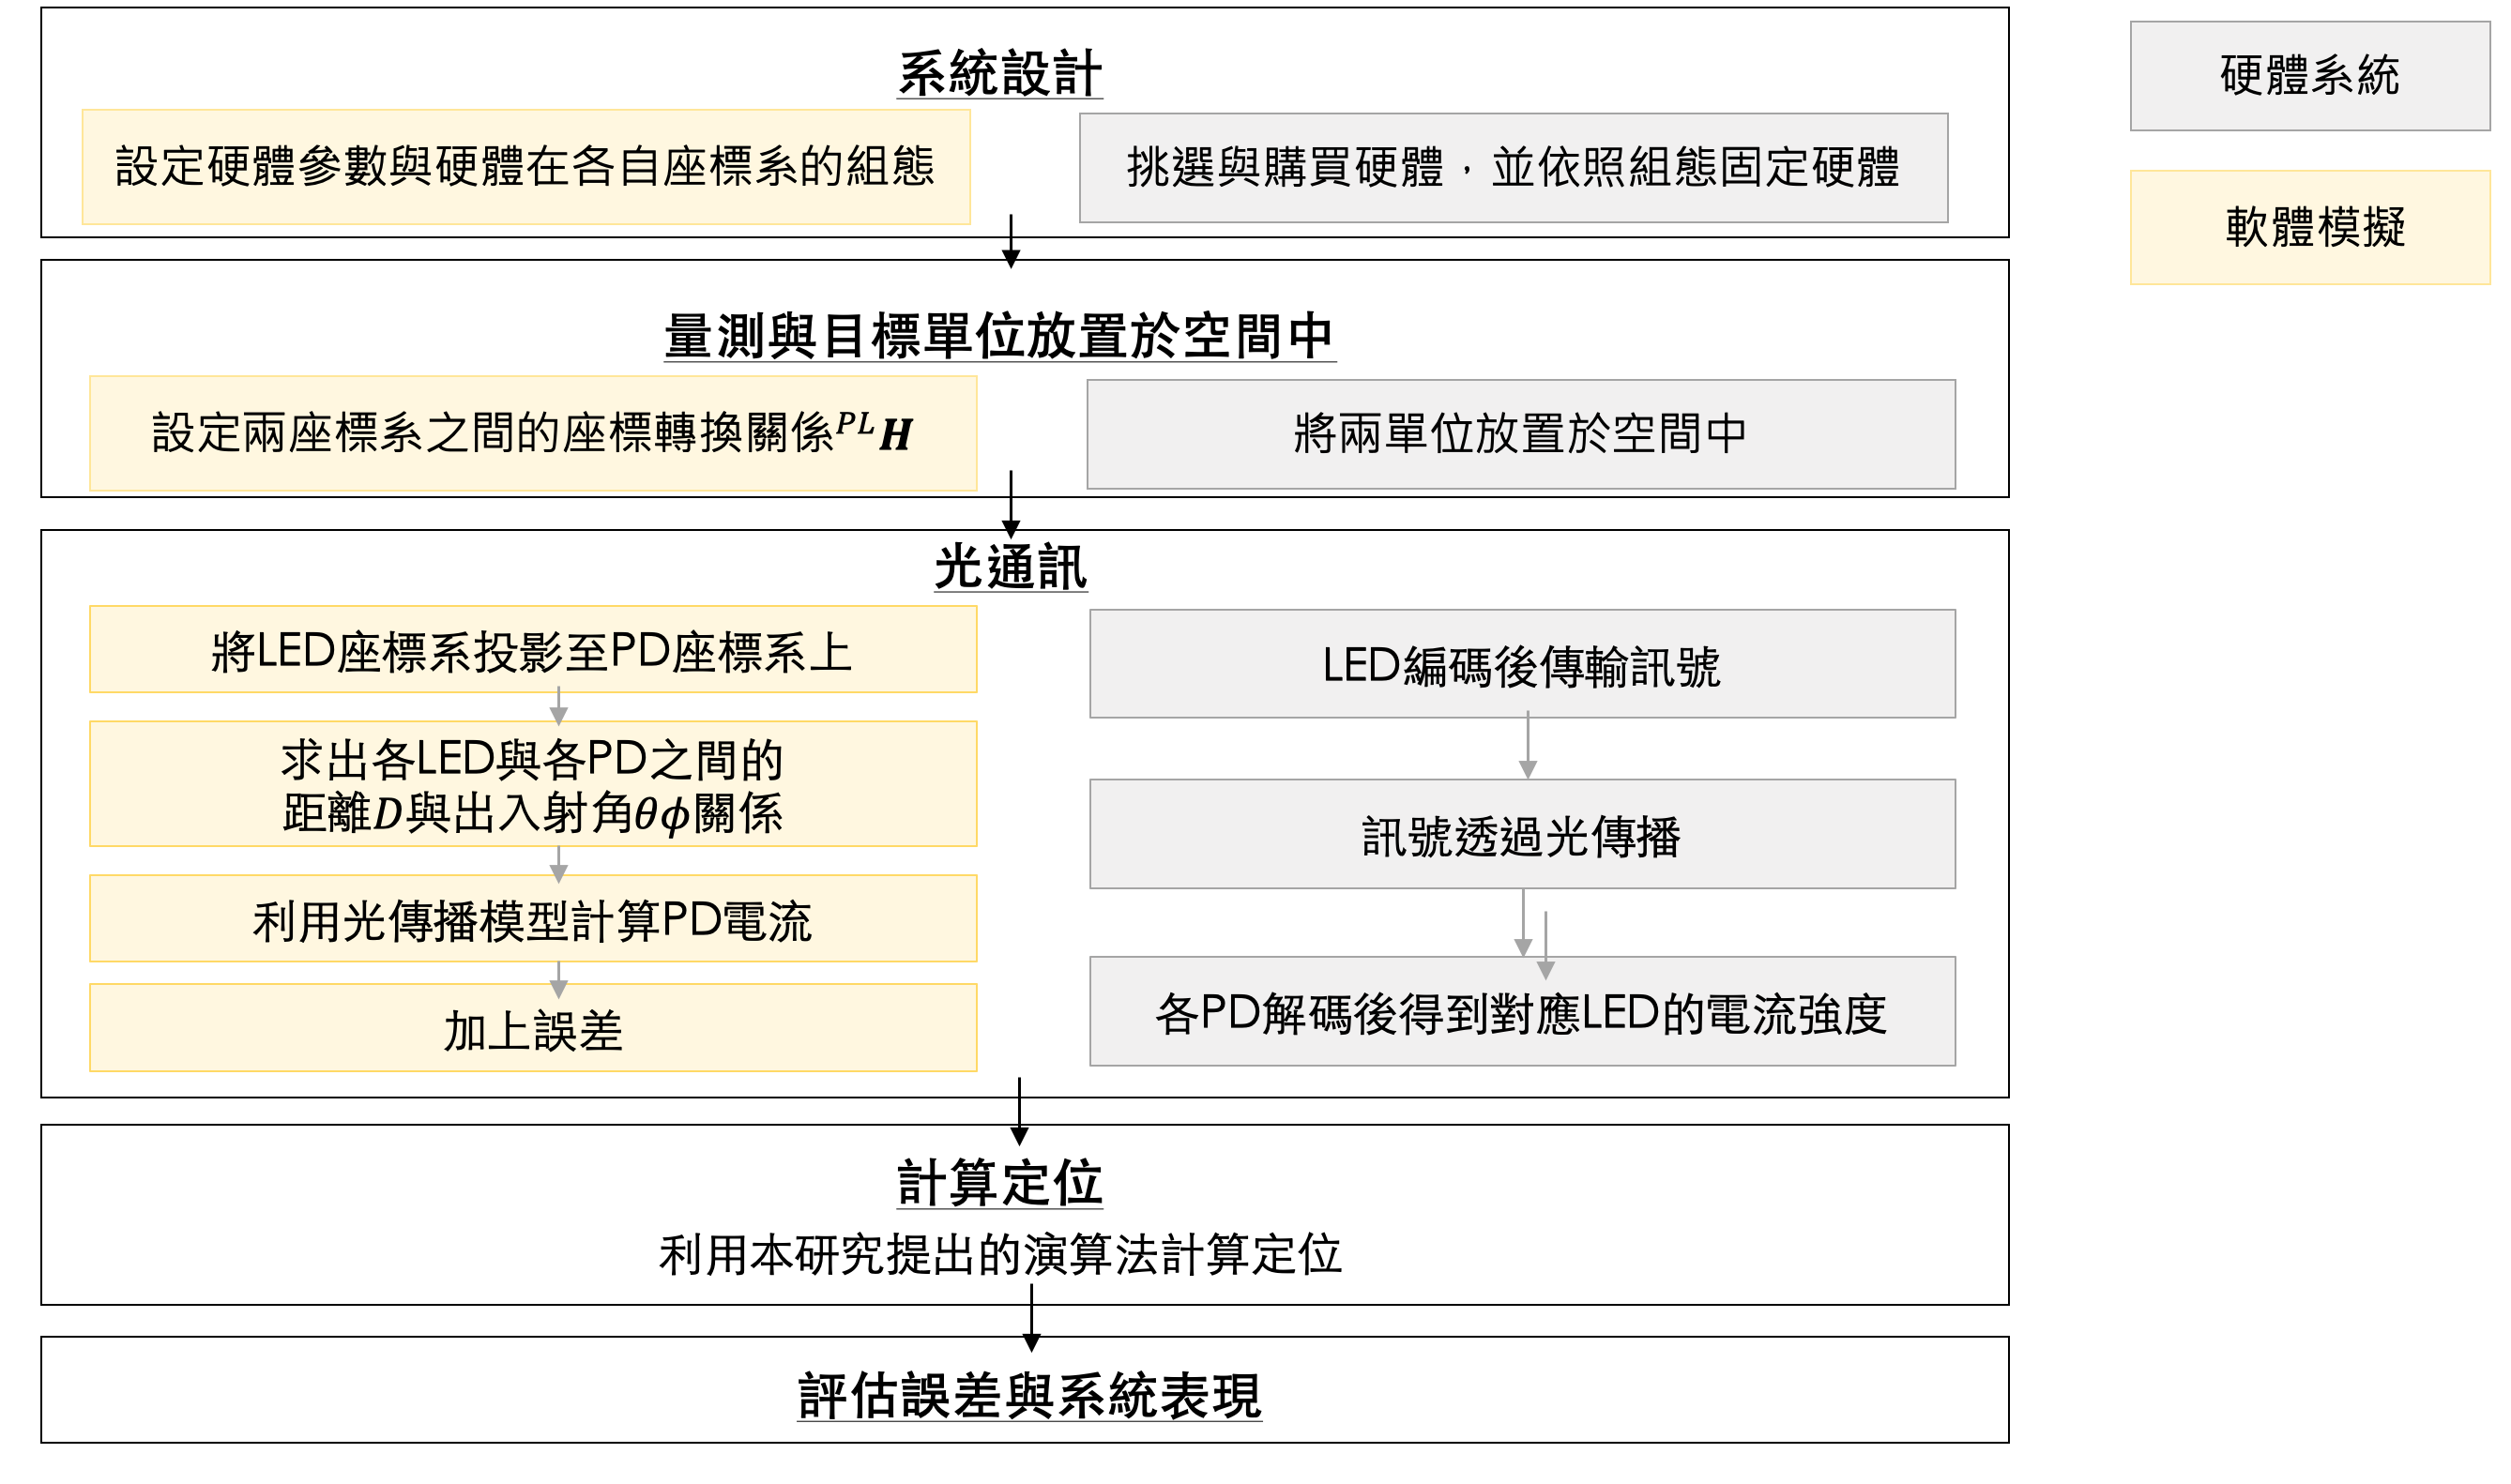
\includegraphics[width=15cm]{ch4pic/simulate_hardware.png}
    \caption{多LED對多PD定位系統以硬體驗證與軟體模擬的流程圖}
    \label{pic:simulate_hardware}
\end{figure}

第三章中,我們提出了一個多LED對多PD系統的演算法,具有獲得三維定位以及目標物姿態的能力,且不需限制目標平面與使用者平面平行,在硬體擺放的指向以及數量上也具有靈活度。而定位演算法的表現,通常會透過架設硬體系統來進行驗證,定位系統的流程可參考圖\ref{pic:simulation_flow}。然而在光通訊發展並不如無線電波段成熟的情況下,架設光通訊系統具有難度,無法直接購買到包裝完整的光通訊套件。因此,大多數的文獻上會透過軟體模擬,建立一虛擬環境將LED與PD系統放至於空間中,將光通訊解碼後的強度資訊模擬輸出,提供給定位演算法計算出相對位置,再針對解出的相對位置誤差對系統表現進行評估。

本章節便會利用軟體模擬的方法,建立一模擬環境,將光通訊的步驟在模擬中完成,再以第三章提出的定位演算法計算出相對位置,並評估誤差與系統表現。以下依序在\ref{chp:simulation}章中詳細介紹模擬方法,並再\ref{chp:scenario}章中介紹模擬的情境,而模擬的結果與分析於\ref{chp:system_perform}章中分析,最後於\ref{chp:4_conclusion}章中總結。

% --------------------------------------
\section{模擬方法}
\label{chp:simulation}

為了針對不同使用情境評估系統表現,模擬流程整理於圖\ref{pic:simulation_flow},其中,由於在評估系統時,需要對不同的使用情境進行設計,因此我們的模擬流程由定義使用情境開始,參考\ref{chp:scenario}章,而根據不同使用情境,量測與目標單位於空間中的相對位置與姿態也會有所不同。系統設計的部分於\ref{chp:hardware_design}章中介紹,需決定的部分包含硬體數量、硬體參數以及硬體組態。有了硬體組態與座標轉換關係,即可透過式\ref{eqn:model_coor_extend}計算出相對位置,如何模擬硬體誤差則在\ref{chp:hardware_error}章中介紹。最後則是透過第三章提出的演算法,計算出相對位置與誤差。


\begin{figure}[ht]
    \centering
    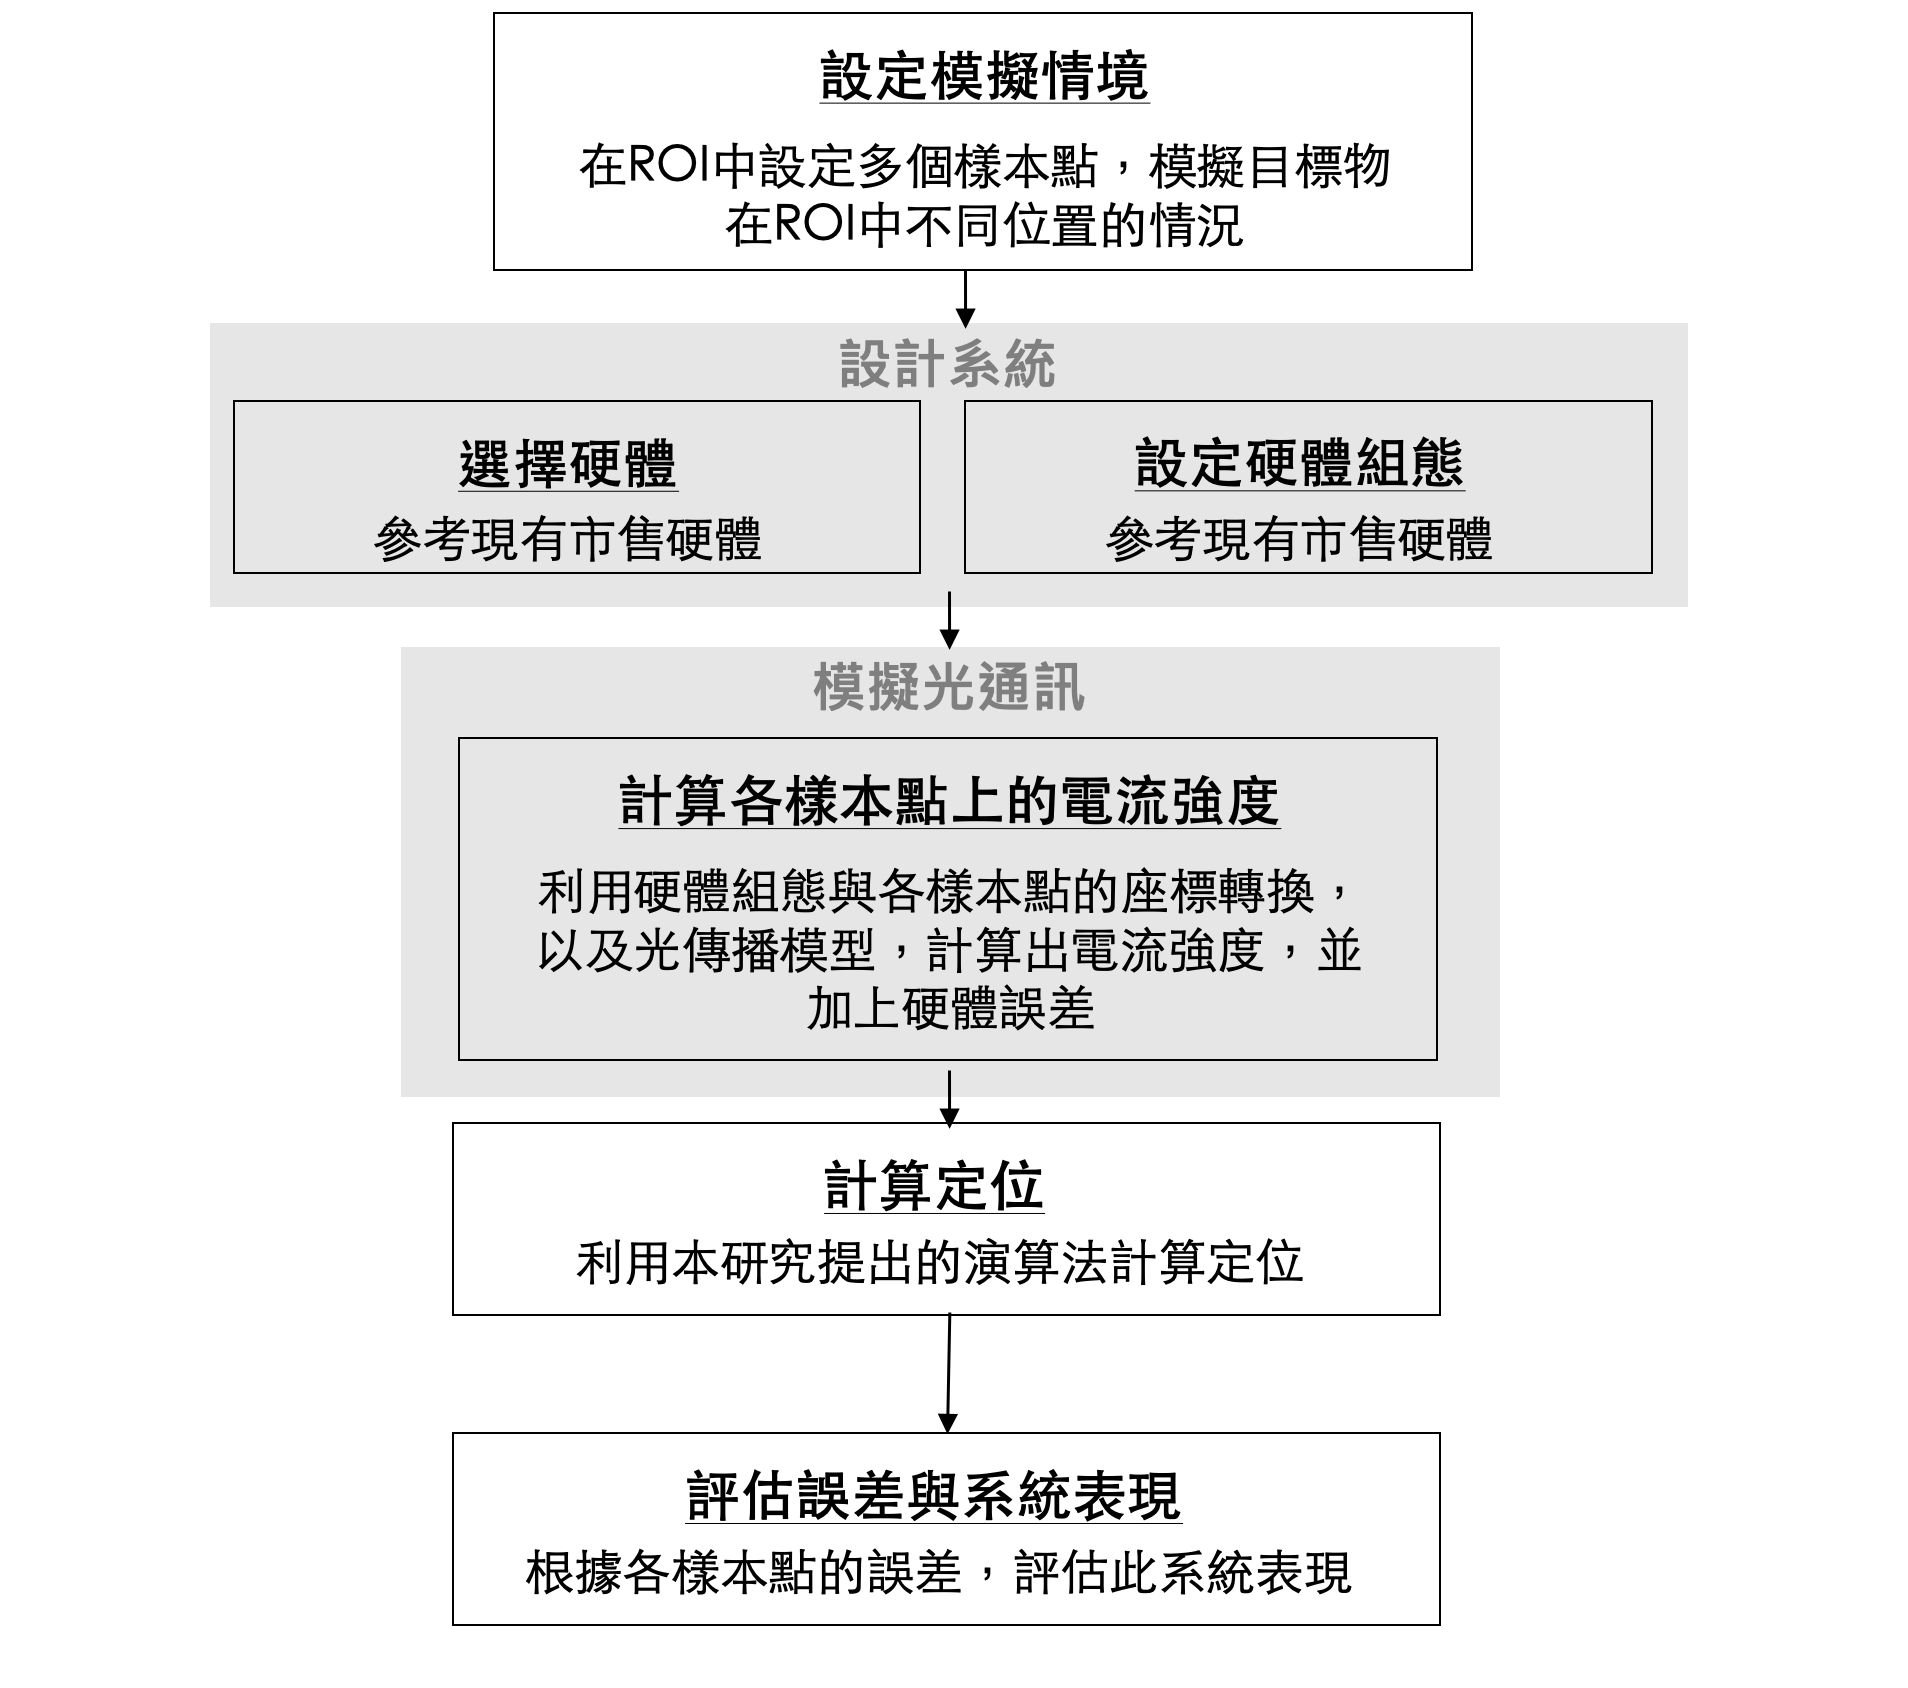
\includegraphics[width=13cm]{ch4pic/simulation_flow.png}
    \caption{模擬流程圖}
    \label{pic:simulation_flow}
\end{figure}

\subsection{定義模擬情境}
\label{chp:scenario}

為了針對不同使用情境評估系統表現,我們於此情境中的感興趣區域(Region of Interest,以下簡稱ROI)中建立多個樣本點,針對第$k$個樣本點中量測出的相對位置$\hat{^{PL}_{k}\boldsymbol{T}}$,計算出與實際相對位置$^{PL}\boldsymbol{T}$的誤差$_k e$,參考圖\ref{pic:error_show}。其中,ROI是相對PD座標系去作定義,也就是將PD視為固定,定義LED座標系相對於PD座標系的座標轉換關係$^{PL}\boldsymbol{H}$。僅定義LED座標系相對於PD座標系的關係之原因,是因為在不考慮環境障礙物情況下,兩座標系的絕對位置並不重要,僅有相對關係會對相對位置造成影響。

\begin{figure}[ht]
    \centering
    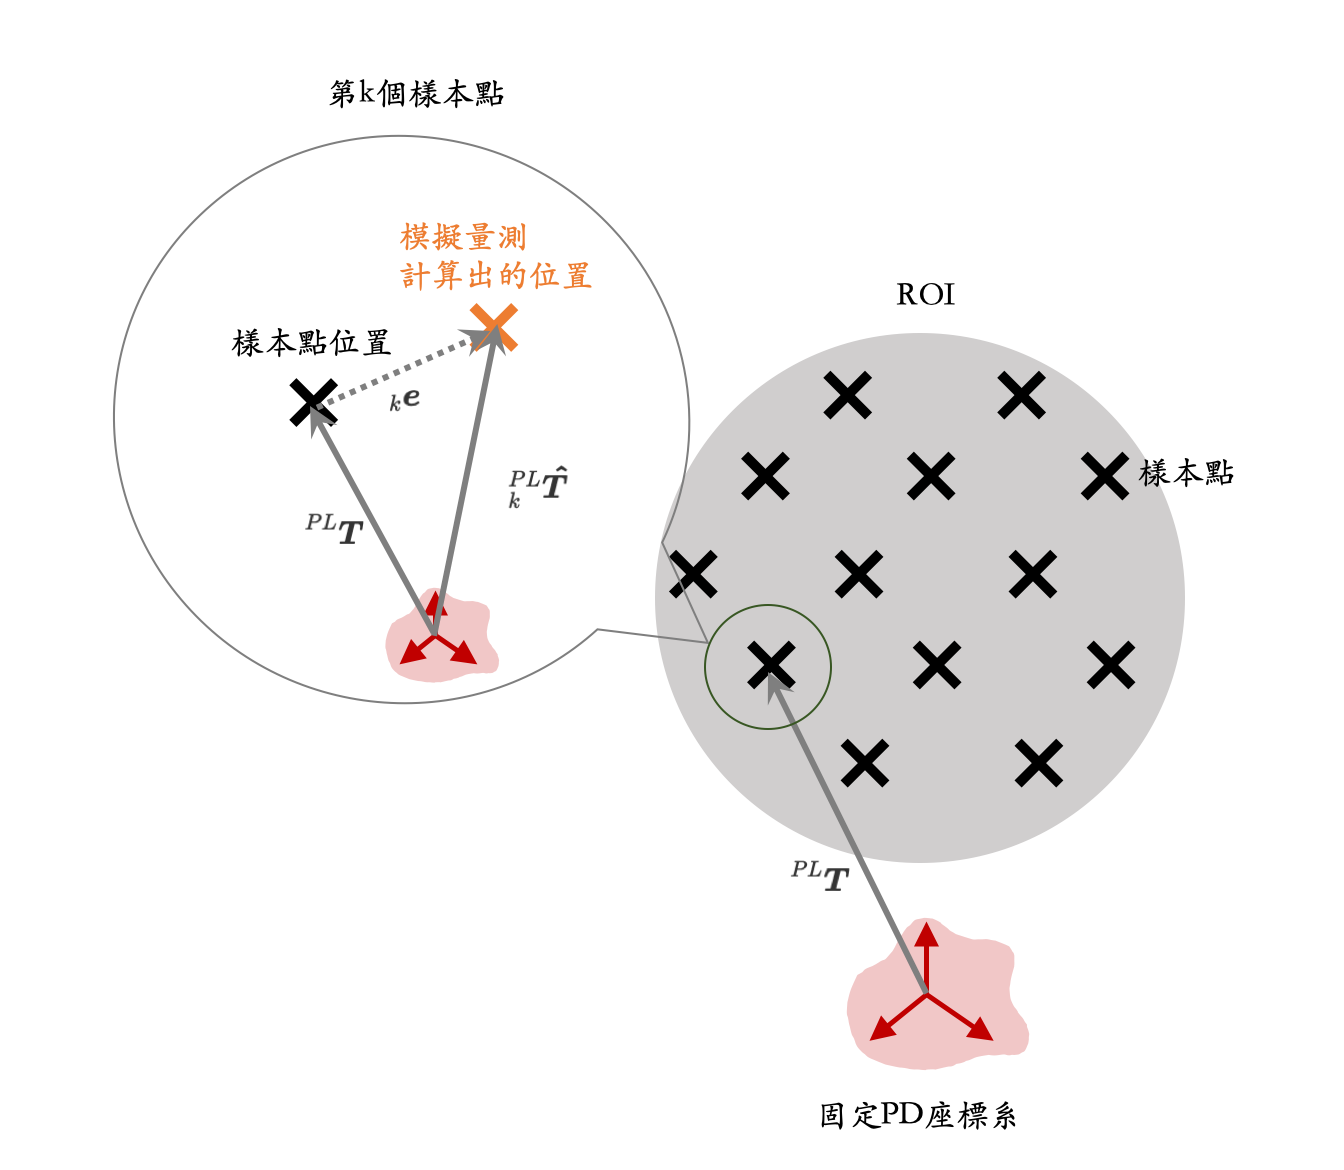
\includegraphics[width=9cm]{ch4pic/error.png}
    \caption{樣本點與誤差}
    \label{pic:error_show}
\end{figure}

在這裡,我們選擇常見的室內定位情境作為模擬情境,也就是目標物LED座標系固定於天花板朝地面照射,而量測者的PD座標系於室內空間中,測試範圍設置的較\cite{case:cart3d}\cite{case:3d_layers}中的都大,為$3 \times 3 \times 3 m$的範圍,如圖\ref{pic:translate_sample}。而由於本研究所使用的演算法並不需限制目標平面與量測平面平行,因此兩座標系之間的姿態也可以改變,除了平移的樣本點還需建立旋轉的樣本點,旋轉樣本點由翻滾(以下稱為Roll)、俯仰(以下稱為Pitch)、偏擺(以下稱為yaw)三個旋轉角度定義,旋轉順序依序為Roll, Pitch, Yaw。旋轉樣本可參考圖\ref{pic:rotate_sample},紅色箭頭代表的是PD座標系Z軸,藍色的各個箭頭則代表與其相對的的LED座標系Z軸,並以極座標圖呈現於圖中。

\begin{figure}[ht]
    \centering
    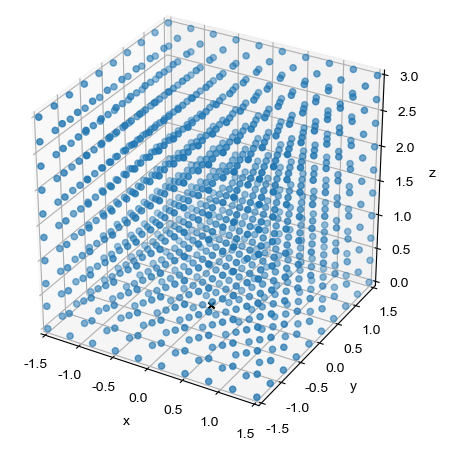
\includegraphics[width=6cm]{ch4pic/translate_sample.png}
    \caption{平移樣本點}
    \label{pic:translate_sample}
\end{figure}

\begin{figure}[ht]
    \centering
    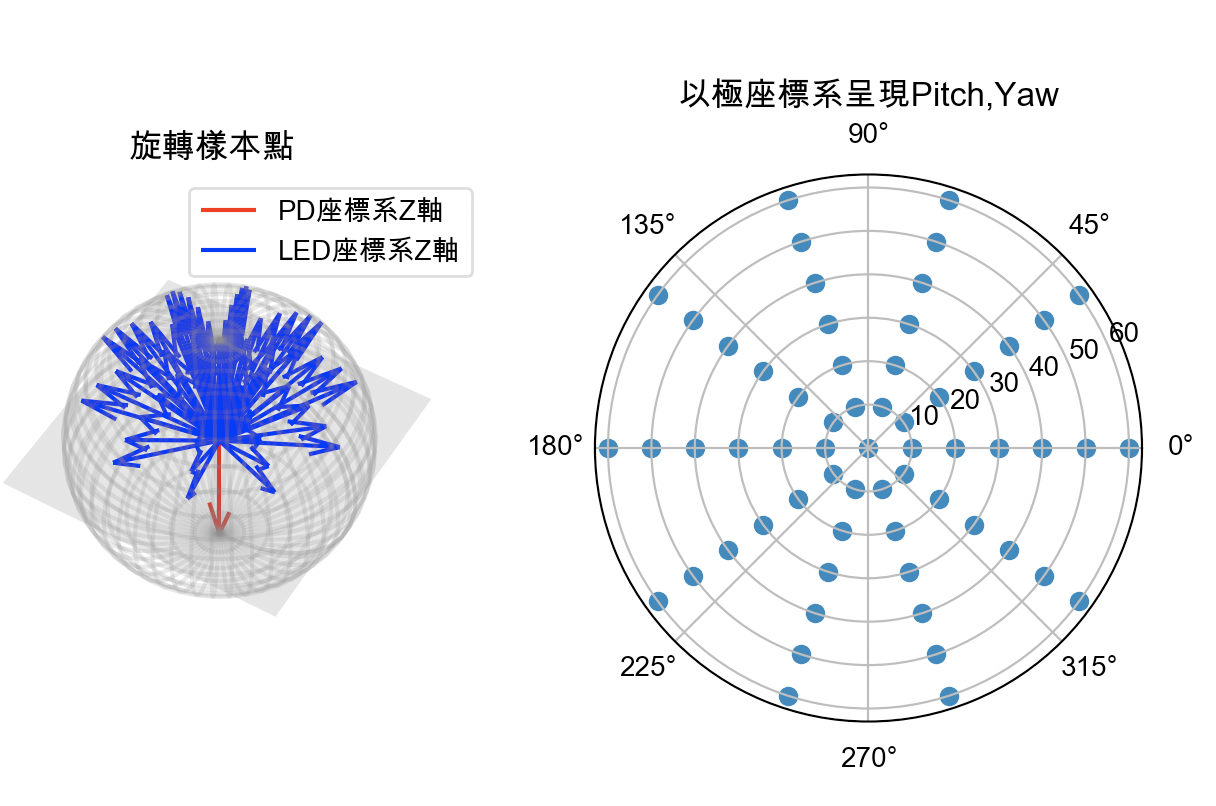
\includegraphics[width=8cm]{ch4pic/rotate_sample.png}
    \caption{旋轉樣本點}
    \label{pic:rotate_sample}
\end{figure}

\begin{table}[h!]
    \begin{center}
      \caption{平移樣本點}
      \label{tab:translate}
      \begin{tabular}{c|c|c|c} % <-- Alignments: 1st column left, 2nd middle and 3rd right, with vertical lines in between
         & \textbf{最小值} & \textbf{最大值}&\textbf{樣本數}\\
        \hline
        $t_x$ & -1.5 & 1.5&10\\
        $t_y$ & -1.5 & 1.5&10\\
        $t_z$ & 0 & 3 &10\\
      \end{tabular}
    \end{center}
  \end{table}

  \begin{table}[h!]
    \begin{center}
      \caption{旋轉樣本點}
      \label{tab:rotate}
      \begin{tabular}{c|c|c|c} % <-- Alignments: 1st column left, 2nd middle and 3rd right, with vertical lines in between
        & \textbf{最小值} & \textbf{最大值}&\textbf{樣本數}\\
       \hline
       Roll & $\pi$ & $\pi$&1\\
       Pitch & $\pi/18$ &$\pi/3$&6\\
       Yaw & $\pi/5$ & $2\pi$&10\\
     \end{tabular}
   \end{center}
 \end{table}

如表\ref{tab:translate}中所示,一共有$10\times 10\times 10$總共一千個平移樣本點,旋轉樣本點則有$1\times 6\times 10$共六十個,兩者相乘代表總共六萬個樣本點。這代表著每個平移樣本點上皆需做出60次旋轉,以旋轉樣本點來看也是,每個旋轉樣本點都需在每個平移樣本點上計算一次。



\subsection{硬體選擇與設計}
\label{chp:hardware_design}

硬體組態的部分,位置的限制如\ref{chp:algorithm_constraint}章中所述,需限制PD擺放位置於PD座標系原點:$^P\boldsymbol{P}_p=
\left[\begin{array}{ccc}0&0&0\end{array}\right]^T$,LED的擺放位置也限制於LED座標系原點:$^L\boldsymbol{P}_l=
\left[\begin{array}{ccc}0&0&0\end{array}\right]^T$。

硬體數量的部分,參考\ref{chp:orient_conclu}章中所述,LED與PD數量各需要最少三個來達成三維定位,因此我們將PD和LED硬體的數量上下限,設計範圍定在三個到十五個之間。

硬體參數的部分,LED參考\cite{datasheet:led_vsma},以供應5A時的輻射強度作參考,取$Pt=1.7\pi W$,而PD則參考\cite{datasheet:BPW},將$Re\times A = 4.2\times10^{-6}$,而兩硬體的朗博次方則都設定為一。


\subsection{誤差模擬方法}
\label{chp:hardware_error}

圖\ref{pic:simulation_flow}流程中,模擬光通訊的部分可透過式\ref{eqn:model_algorithm_filter}獲得,而為了更真實的模擬現實狀況,參考\cite{survey_light2018}中對誤差的模擬,呈現於式\ref{eqn:noise}中,$\hat{Ie}_{lp}$代表第l個LED對第p個PD的量測電流,其組成包含了理想的量測電流$Ie_{lp}$與PD硬體誤差。PD硬體誤差中,又可分為熱雜訊$It$(Thermal Noise)與散粒雜訊$Is$(Shot Noise),各自呈現於式\ref{eqn:thermal_noise}與式\ref{eqn:shot_noise}中,其中$Kb$為波茲曼常數(Boltzmann constant)、$Te$為絕對溫度、$B$為頻寬、$Rs$為分路電阻(Shunt Resistance)、$q$為電子電荷。

\begin{equation}
\label{eqn:noise}
    \hat{Ie}_{lp}=Ie_{lp}+\sqrt{It_{lp}^2+Is_{lp}^2} 
\end{equation}


\begin{gather}
    \label{eqn:thermal_noise}
    It_{lp}=\sqrt{\frac{4 Kb Te B}{Rs}}\\
    \label{eqn:shot_noise}
    Is_{lp}=\sqrt{2qIe_{lp}B}
\end{gather}

% --------------------------------------



% --------------------------------------
\section{評估系統表現}
\label{chp:system_perform}



根據以上設定,我們將六萬個樣本點進行定位,然而,各樣本點都有可能遇到無法求解的狀況,如\ref{chp:orient_conclu}章所提到,若沒有任何一個LED同時將訊號傳送給三個以上的PD,則無法解出方位;而若沒有任何一個PD同時接受到三個以上LED資訊,則無法計算距離。即使我們今天系統設計有超過三個以上的LED與PD硬體數量,在\ref{chp:algorithm_filter}章中也會將訊號過大、過小的數值去除,導致所得訊號不足求解的狀況。在各樣本點可能會解不出來的情況下,解不出來則會完全無法計算誤差,因此無法利用樣本點平均誤差來完整描述系統的表現。

因此,我們改看「在容許範圍$To$(Tolerance)」內的樣本點比例,在這邊我們設定$To=0.1m$,而結果呈現於圖\ref{pic:sample_out}。

\begin{figure}[ht]
    \centering
    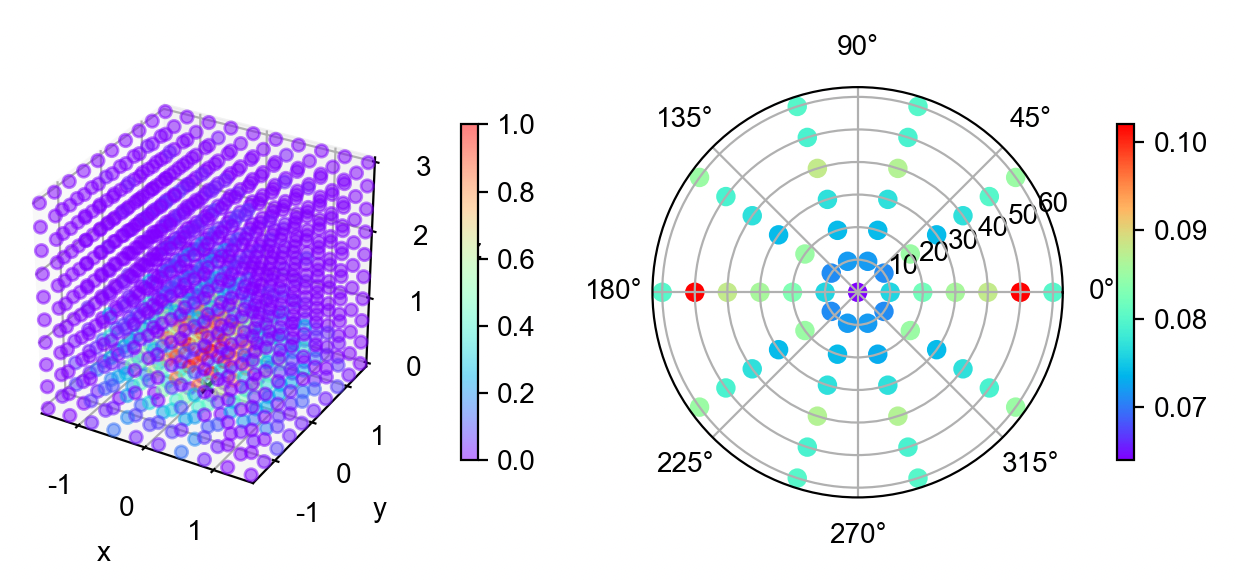
\includegraphics[width=9cm]{ch4pic/sample_out.png}
    \caption{容許範圍內的樣本點比例}
    \label{pic:sample_out}
\end{figure}

觀察圖中的現象,在PD座標系延伸出去,有一橢圓區塊具有很高的定位能力,定位能力的分佈與其他文獻符合。

而由於第三章此演算法並沒有限制硬體數量、朗博次方與硬體指向,在設計上是有靈活度的,因此我們透過改變這幾項變數,來觀察系統的反應。其中,LED與PD指向的部分,我們將每個硬體皆具有的兩個由度限制剩下一個,假設方位角平均分配:$^P\beta_p = 2\pi/P$、$^L\beta_l = 2\pi/L$,仰角的部分則限制必須相同$^P\alpha_p =^P\alpha$、$^L\alpha_l = ^L\alpha$。在這樣的限制下,我們分別探討各項變數的影響。



\subsection{朗博次方的影響}

在假設$^P\alpha_p =\pi/18$、$^L\alpha_l = \pi/18$,以及硬體數量$L=P-8$的情況下,我們改變朗博次方,並將樣本中於容許範圍內的比例,呈現於圖\ref{pic:m_translate}與圖\ref{pic:m_rotate}中。隨著朗博次方的提升,硬體所照射的範圍越來越小,因此容許範圍內比例高的的區域便越顯集中。

\begin{figure}[h!]
    \centering
    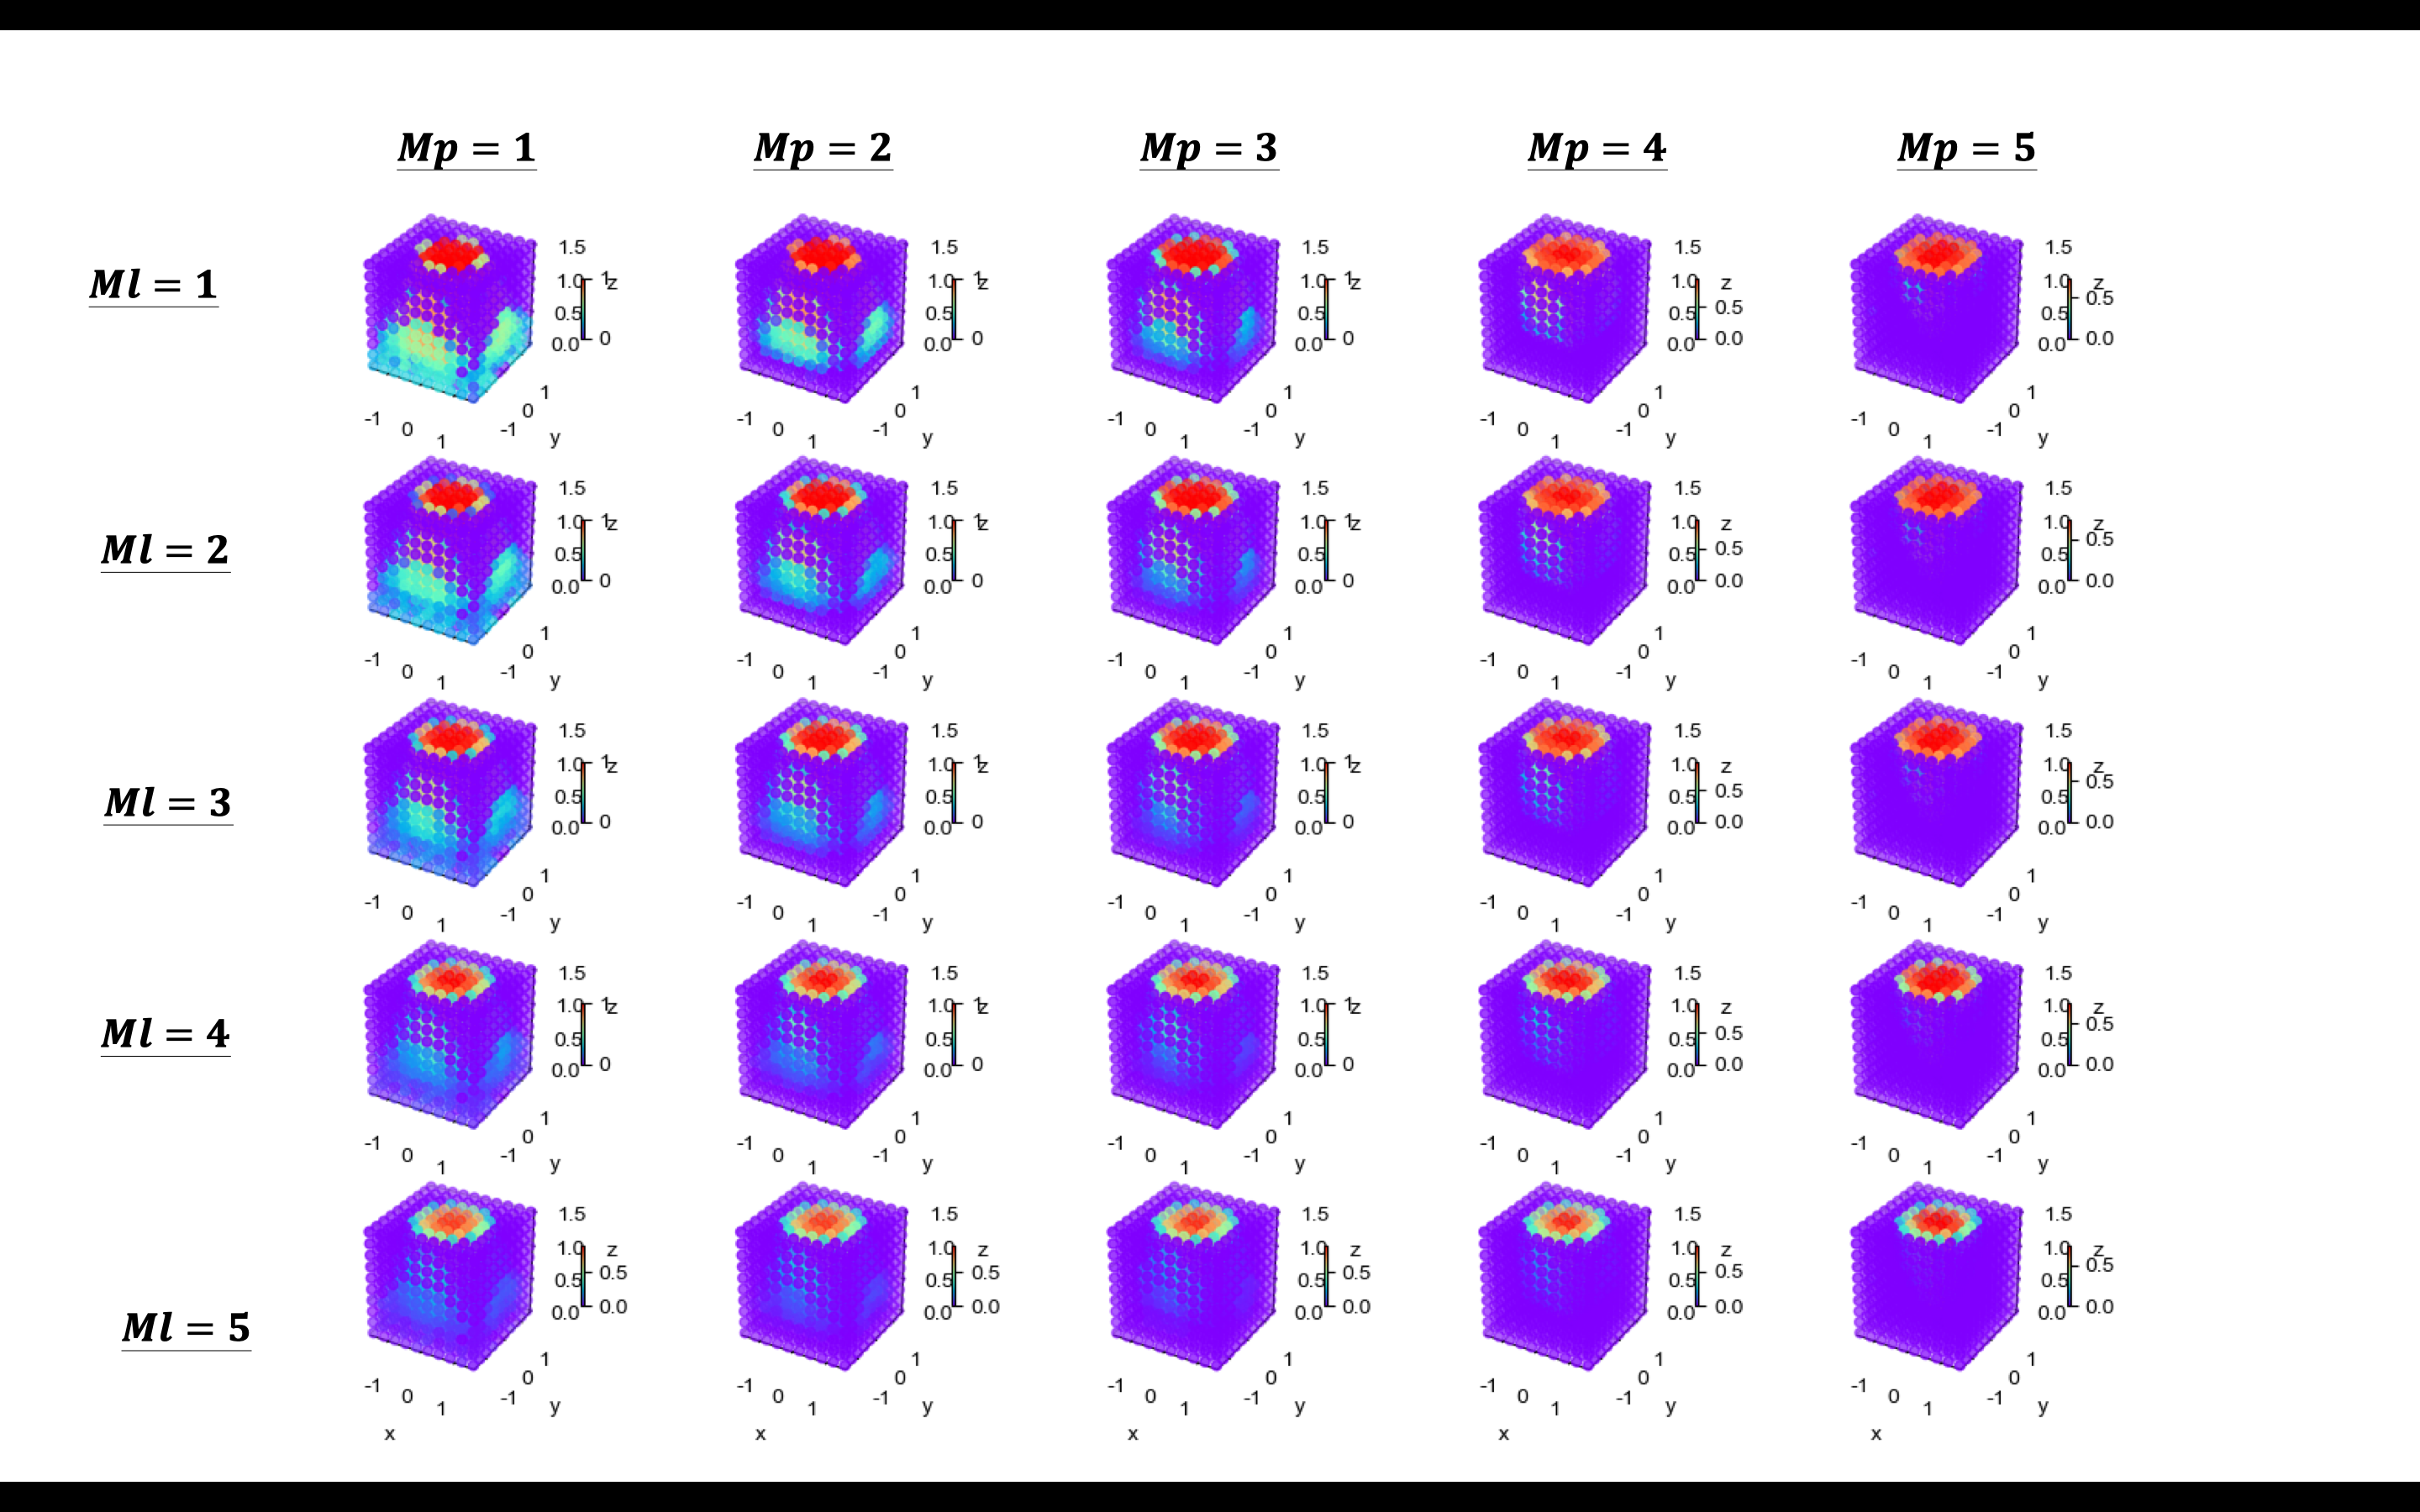
\includegraphics[width=14cm]{ch4pic/m_translate.png}
    \caption{改變朗博次方對平移樣本點的影響}
    \label{pic:m_translate}
\end{figure}
\begin{figure}[h!]
    \centering
    \includegraphics[width=14cm]{ch4pic/m_rotate.png}
    \caption{改變朗博次方對旋轉樣本點的影響}
    \label{pic:m_rotate}
\end{figure}

我們將平移與旋轉樣本點總共六萬個點中,在容許範圍內的比例,呈現於圖\ref{pic:m_effect},我們可以觀察到在此情境中,較小的朗博次方使系統表現較佳。

\begin{figure}[h!]
    \centering
    \includegraphics[width=9cm]{ch4pic/m_effect.png}
    \caption{改變朗博次方對系統的影響}
    \label{pic:m_effect}
\end{figure}



\subsection{LED與PD指向的影響}

在假設朗博次方$Mp=M\ell=1$,以及硬體數量$L=P-8$的情況下,我們改變硬體指向$^P\alpha,^L\alpha$,並將樣本中於容許範圍內的比例,呈現於圖\ref{pic:alpha_translate}與圖\ref{pic:alpha_rotate}中。隨著硬體指向提升,多個硬體之間重疊的覆蓋範圍便越來越小,漸漸僅剩下於中心位置的樣本點:$x,y,=0$。

\begin{figure}[h!]
    \centering
    \includegraphics[width=14cm]{ch4pic/alpha_translate.png}
    \caption{改變硬體指向對平移樣本點的影響}
    \label{pic:alpha_translate}
\end{figure}
\begin{figure}[h!]
    \centering
    \includegraphics[width=14cm]{ch4pic/m_rotate.png}
    \caption{改變硬體指向對旋轉樣本點的影響}
    \label{pic:alpha_rotate}
\end{figure}

我們將平移與旋轉樣本點總共六萬個點中,在容許範圍內的比例,呈現於圖\ref{pic:alpha_effect},我們可以觀察到在此情境中,較小的硬體擺設天頂角,使系統表現較佳。

\begin{figure}[h!]
    \centering
    \includegraphics[width=9cm]{ch4pic/m_effect.png}
    \caption{改變硬體指向對系統的影響}
    \label{pic:alpha_effect}
\end{figure}



\subsection{LED與PD數量的影響}

由圖\ref{pic:m_effect}與圖\ref{pic:alpha_effect}中,我們都可以看出在提高硬體數量時,系統表現提升,然而系統表現提升的幅度不與硬體提升的數量成正比。因此,在挑選硬體數量時,除了系統表現以外,也需將硬體增加所造成的硬體成本,以及架設系統的難度考慮進來,在系統表現與硬體系統簡單中取捨。

% --------------------------------------
\section{結論}
\label{chp:4_conclusion}


由以上分析,我們可以看出在\ref{chp:scenario}章中提出的情境下,小的朗博次方與較小的硬體天頂角$\alpha$使系統的表現較佳,而硬體數量則是愈多愈好,但成長的趨勢隨著硬體數量增多而減慢。

我們本章節提出的方法,可以在軟體中透過改變硬體的選擇、樣本點的集合、組態等,快速的對不同情境,評估不同系統設計的表現。有了此模擬方法,我們可以在硬體系統架設之前對系統表現有所了解,避免在硬體架設的部分浪費時間與硬體成本。除此之外,藉由可以分析不同設計下的系統表現,我們進而於第五章針對不同情境,進行朗博次方、硬體指向以及硬體數量的最佳化,提供特定使用情境下的最佳系統設計。
\chapter{針對不同使用情境最佳化組態與朗博次方}
\label{chp:5}


\section{簡介}

此章節要針對特定情境進行最佳化,希望針對該情境,藉由調整LED與PD的硬體參數以及擺放位置,改善系統的量測表現,流程圖如\ref{flow:opt}。

\begin{figure}[ht]
    \centering
    \includegraphics[width=13cm]{ch4pic/flowchart_opt.png}
    \caption{最佳化流程圖}
    \label{flow:opt}
\end{figure}

\clearpage

\subsection{情境設定}

需先定義此量測工況中觀察者座標系的ROI(Region of Interest),擁有此資訊後,將此範圍切割成數個樣本點位置(圖\ref{pic:testpoint})。我們將觀察者的PD座標系固定,將目標物的LED座標系放置於各樣本點,所有樣本點的平均誤差即為量測表現,誤差愈小代表量測表現愈好。

\begin{figure}[ht]
    \centering
    \includegraphics[width=8cm]{ch3pic/testpoint.jpg}
    \caption{ROI與樣本點示意圖}
    \label{pic:testpoint}
\end{figure}

\clearpage

\subsection{目標函數}

愈改善之目標為系統表現,期望能降低系統在ROI中的平均量測誤差,因此由\ref{eqn:objective}表示,將$K$個樣本點中的模擬量測相對位置與標準相對位置相減後,總和除$K$則得平均誤差;其中標準相對位置,為各樣本點相對PD座標系的位置;而模擬量測位置則利用第三章的方式進行數據處理所得。


(參考\ref{flow:opt})

\begin{figure}[ht]
    \centering
    \includegraphics[width=8cm]{ch4pic/error.png}
    \caption{誤差示意圖}
    \label{pic:error}
\end{figure}


\begin{equation}
    \label{eqn:objective}
    \underset{^{P}P_p, ^{L}P_l,^{P}N_p, ^{L}N_l,Ml_l,Mp_p,A_p,Re_p,Pt_l}{\operatorname{minimize}} 
    \quad f = 
    \frac{\sum_{i=1}^{K}(||^{PL}_k\boldsymbol{T} -\hat{^{PL}_k\boldsymbol{T} } ||)}{K}  \\
\end{equation}


\begin{align*} \text{where }
    &p=1,2,...,P\\&l=1,2,...,L
\end{align*}



\subsection{最佳化變數}

硬體參數:$M_l,m_p,A_p,Re_p,Pt_l$

擺設方式:$^{P}P_p, ^{L}P_l,^{P}N_p, ^{L}N_l$

\begin{figure}[ht]
    \centering
    \includegraphics[width=12cm]{ch4pic/variable.png}
    \caption{最佳化變數}
    \label{pic:variable}
\end{figure}
\chapter{結論}
\label{chp:6}


\section{研究總結}


為了用可攜式單位達到一單點對單點的三維定位系統,以達到靈活安裝於不同環境與位置的需求,本研究由探討不同室內定位技術與方法的特性開始,根據需求將目標聚焦在具有以可攜式單位進行三維定位潛力的LED與PD定位系統上。然而,此領域中現有文獻大多利用情境限制與硬體組態限制來簡化系統複雜度,例如限制量測者與目標物平面平行、忽略朗博次方、限制硬體擺設方法等。這些限制除了降低了次系統設計的自由度外,也使應用情境大大的受限,與我們的目標不符。因此,為了解決此領域中應用情境與次系統設計過多的限制,本研究於第三章建立一廣用於三維空間中的三維定位演算法,在不限制量測者與目標物平面平行的情況下,達到三維定位並可得到目標物姿態,且該演算法完整考量朗博次方,並將LED與PD的硬體數量與各硬體的擺設指向視為變數,提供LED與PD系統更具靈活度的應用可能。

除了建立一廣用於三維空間中的定位演算法,本研究於第四章建立多LED對多PD的定位模擬系統,可透過簡單的調整參數,以對不同次系統規格、不同使用情境與ROI、以及不同誤差模擬方式,進行系統成效的量化評估。為了凸顯本研究演算法與其他文獻之差異,於\ref{chp:design_result}章中提出一使用情境,其擁有$3\times 3\times 3m$的平移樣本空間與61種旋轉姿態作為樣本點,以此模擬目標平面與量測平面不需平行之移動行為。透過分別調整不同次系統設計參數、誤差模擬等參數,我們可以分析各參數對此使用情境系統效能的影響;除了該情境外,也於\ref{chp:scene_effect}中提出另外三個使用情境,得到不同使用情境會有不同系統成效的結論且各參數的影響也不盡相同,系統的複雜度很高,也凸顯了針對不同情境進行最佳化有其必要性。

因此,對各項變數與系統成效的關係有基本了解之後,本研究於第五章中建立一最佳化流程,針對不同情境進行次系統設計的最佳化,透過指定硬體數量的設計空間,將設計空間中的朗博次方與各硬體的指向進行最佳化,提供針對該情境最合適的次系統規格,讓使用者在實際進行硬體系統建立之前,得以對系統表現有基本的理解,並以此最佳化結果作為硬體系統搭建的參考依據。本章節使用三個使用情境作為最佳化案例,以最佳化結果來看,各情境中得出的最佳次系統設計十分不同,也顯示出次系統設計的重要性。

總而言之,LED與PD的定位方法具有以可攜式單位進行三維定位的潛力,而系統具有靈活度的同時複雜度也高,透過改變次系統設計、改變使用情境、改變模擬參數,都會使定位成效有所不同。因此,提出廣用於三維空間的定位演算法是為提供使用者一單點對單點進行三維定位的可能性;而模擬與評估方法提供了一有效率的方法對此複雜的系統進行量化評估,讓使用者得以用方便的模擬軟體對複雜的系統有所了解;至於最佳化方法則是針對特定使用情境提供最合適的次系統設計,除了可以了解此使用情境的極限外,也能作為硬體搭建的設計參考。


% 本研究建立一分析流程,將資料數量龐大的模擬模型軌跡與有限資料點的真實系統軌跡,經前處理後獲得兩等量等距結果,並進一步透過位置資訊序列與角度資訊序列,建立仿射轉換與輪廓差異指標後,得到單一複合指標,量化模擬模型與真實系統軌跡,提供模型驗證更多有效資訊進行調整。並透過一三輪車模型案例,利用閉迴路系統產生模擬模型軌跡,以及開迴路系統加入偏差參數獲得真實系統軌跡,計算差異量化指標後,以有效替代模型進行參數估測,驗證該複合指標的有效性,同時,對於有雜訊軌跡提供調整建議,提升方法可行性。

% 越接近真實系統的電腦模型,能使工程師更加掌握真實系統樣貌。而在模型驗證領域,對於軌跡動態輸出量化有其必要性,透過量化指標可以定量地衡量系統與參數間的關係,並得到量化差異結果進一步修正系統或調整參數。本研究提出的複合量化指標,可以針對不同操作軌跡模型進行差異量比較,也在實驗案例中,提出替代模型的概念,進一步使用量化指標達到參數估測的目的。

\section{未來目標}


\begin{description}

    \item[- 提升演算法靈活度:] 第\ref{chp:3}章提出的演算法中,仍然有限制硬體種類需相同,侷限了硬體挑選以及系統設計上的自由度。透過調整演算法可解除此限制,繼續提升演算法靈活度,然而演算法複雜度也隨之提升,需特別注意。
    
    \item[- 提升模擬真實度:] 本研究與大多LED對PD的定位系統相同,在模擬中並沒有考量多重路徑誤差、干涉等效果的誤差,因此不夠貼近實際系統的表現。無論是以實驗評估誤差,或是將模擬系統加入更多誤差考量,便可檢考模擬與實際系統的差異。
    
    \item[- 硬體驗證:]本研究與大多LED對PD的定位系統相同,缺乏硬體驗證,僅利用模擬評估演算法與誤差;然而模擬與實際情況必有出入,最正確評估系統的方式便需架設完整的光通訊系統,並利用該系統進行定位,針對實驗結果再進行分析與研究以調整演算法或是系統設計。
    
    

\end{description}


\chapter{附錄:程式碼說明}

\hspace*{-3cm}\includegraphics[width=22cm]{ReadMe.pdf}



%----------- Input your appendix here  -----------
% \appendix
% \titlecontents{chapter}[0em]{\fontsize{12}{18}\selectfont}
%   {\hspace{3.5em}\contentslabel[附錄\,\thecontentslabel]{3.5em}}
%   {}{\hspace{0.5em}\titlerule*{.}\contentspage}

% \titleformat{\chapter}[display]
% 	{\bf\Large}
% 	{\filleft 附錄\,\thechapter}
% 	{1ex}
% 	{\huge\titlerule
% 	 \vspace{2ex}%
% 	 \filright}
% 	[\vspace{2ex}%
% 	 \titlerule]

% \includepdf[pages={1}]{ReadMe.pdf}
% \onehalfspacing



\backmatter


%---------- Input your reference here ---------
% \bibliographystyle{ieeetr}
\bibliographystyle{unsrt}
\addcontentsline{toc}{chapter}{\bibname}
\bibliography{thesisbib.bib}

%----------- Input your Figure chapter here  -----------
%\input{EndFigTab} 
%chapter cite  == \include
%\include{EndFigTab}

\end{document}
